%% Informe de Trabajo de Título — basado en la plantilla oficial INFO-1197 (UCT)
%% Estructura del cuerpo según la Figura 3.1 de la guía de Cardiff, adaptada a la Etapa 1.
\documentclass[12pt,oneside,spanish,oldfontcommands]{memoir}
\usepackage[backend=biber,style=apa]{biblatex}
\addbibresource{referencias.bib}
\DeclareLanguageMapping{spanish}{spanish-apa}
\usepackage{mathpazo}
\usepackage[T1]{fontenc}
\usepackage[utf8]{inputenc}
\setcounter{secnumdepth}{3}
\setcounter{tocdepth}{2}
\setlength{\parskip}{\medskipamount}
\setlength{\parindent}{0pt}
\usepackage{babel}
\usepackage{booktabs}
\usepackage{float}
\usepackage{url}
\usepackage{array}
\usepackage{textcomp}
\usepackage{graphicx}
\usepackage{rotating}   %% sidewaysfigure: diagramas de secuencia anchos, apaisados en el anexo
\usepackage{csquotes}
\usepackage{longtable}
\usepackage{multirow}
\usepackage[table]{xcolor}
\usepackage{adjustbox}   %% regla permanente: \begin{tablaseg}...\end{tablaseg} nunca desborda
\newenvironment{tablaseg}{\begin{adjustbox}{max width=\linewidth,center}}{\end{adjustbox}}
\usepackage{tikz}
\usetikzlibrary{positioning,shapes.geometric,arrows.meta,fit,backgrounds,calc,decorations.pathreplacing}
\usepackage{hyperref}
\hypersetup{pdftitle={Sistema integrado para el registro, gestión y monitoreo de dispositivos IoT},
  pdfauthor={Vicente Ricardo Ramírez Oñate}, pdfsubject={Trabajo de Título INFO-1197, Etapa 3}, pdflang={es-CL}}
\usepackage[none]{hyphenat}
\sloppy

%% ---- leyendas estilo APA: «Figura N. Texto.» ----
\captionnamefont{\small\bfseries}
\captiontitlefont{\small}
\captiondelim{. }

%% ---- paleta y utilidades compartidas con los documentos del repositorio ----
\definecolor{azuloscuro}{HTML}{1F3A5F}
\definecolor{verdeacento}{HTML}{2E7D5B}
\definecolor{ambar}{HTML}{B06A1F}
\definecolor{grisclaro}{HTML}{F2F4F3}
\definecolor{grislinea}{HTML}{C9D1CC}
\definecolor{gristexto}{HTML}{55635B}
\newcolumntype{L}[1]{>{\raggedright\arraybackslash}p{#1}}
\newcolumntype{C}[1]{>{\centering\arraybackslash}p{#1}}
\newcommand{\encab}[1]{\textcolor{white}{\textbf{#1}}}
\newcommand{\filaencab}{\rowcolor{azuloscuro}}
\renewcommand{\arraystretch}{1.2}

\tikzset{
  caja/.style={draw=azuloscuro, fill=white, line width=0.7pt, rounded corners=2pt,
    align=center, inner sep=5pt, font=\footnotesize},
  cajaacento/.style={caja, draw=verdeacento, line width=1.1pt},
  cajaambar/.style={caja, draw=ambar, line width=1.1pt},
  grupo/.style={draw=grislinea, fill=grisclaro, line width=0.6pt, rounded corners=3pt, inner sep=8pt},
  etiqueta/.style={font=\scriptsize\bfseries\color{gristexto}, align=right},
  flecha/.style={-{Stealth[length=2.4mm]}, line width=0.7pt, color=gristexto},
  flechagruesa/.style={-{Stealth[length=3mm]}, line width=1.1pt, color=verdeacento},
  nota/.style={font=\scriptsize\color{gristexto}, align=center},
  campo/.style={draw=azuloscuro, line width=0.7pt, minimum height=7mm,
    align=center, font=\ttfamily\small, inner sep=3pt},
  notaclave/.style={draw=verdeacento, fill=verdeacento!6, line width=0.9pt, rounded corners=2pt,
    align=left, inner sep=7pt, font=\scriptsize},
  notaaviso/.style={draw=ambar, fill=ambar!6, line width=0.9pt, rounded corners=2pt,
    align=left, inner sep=7pt, font=\scriptsize},
}
%% las figuras compartidas usan estos alias
\newenvironment{cajaclave}[1][]{\par\smallskip\begin{quotation}\small}{\end{quotation}\smallskip}
\providecommand{\captionof}[2]{}

% TeX Live 2025 (kernel 2025-11-01): un paquete engancha \@makecaption y memoir la define de una forma
% que el núcleo no puede re-tokenizar («Generic hooks cannot be added»). Se envuelve en una definición
% limpia y equivalente para que el gancho se instale. Sin esto latexmk termina con error aunque genere PDF.
\makeatletter
\let\memoir@orig@makecaption\@makecaption
\long\def\@makecaption#1#2{\memoir@orig@makecaption{#1}{#2}}
\makeatother

\begin{document}
\sloppy
\vspace*{-6\baselineskip}
\pagenumbering{gobble}
\hspace*{-0.0\textwidth}
\includegraphics[width=\textwidth]{images/Logo_depto_ing_informatica.png}\nonumber

\vspace{2.2cm}

\begin{center}
\textbf{SISTEMA INTEGRADO PARA EL REGISTRO, GESTIÓN\\
Y MONITOREO DE DISPOSITIVOS IoT}\\[0.5cm]
{\small Caso de validación: Campus Dr. Luis Rivas del Canto,\\
Universidad Católica de Temuco}
\end{center}
\vspace{2.2cm}

\begin{center} por \par\end{center}

\begin{center}
VICENTE RICARDO RAMÍREZ OÑATE\vspace{2.2cm}
\par\end{center}

\begin{center}
Trabajo de Título presentado a la\\
Facultad de Ingeniería de la Universidad Católica de Temuco\\
Para Optar al Título de Ingeniero Civil Informático.\\[0.7cm]
{\small Curso INFO-1197 · Profesor guía: Mario Villanueva\\
\textbf{Etapa 2}: Diseño e Implementación Inicial\\
Entrega: 2 de octubre de 2026}
\par\end{center}
\begin{center}
- Temuco, octubre 2026 -
\par\end{center}
\clearpage

%% Comisión, profesor guía/informante y agradecimientos corresponden al documento final:
%% \include{Comision} \include{ProfesorGuia} \include{ProfesorInformante} \include{Agradecimientos}

\pagenumbering{roman}
\tableofcontents{}
\clearpage
\listoffigures
\clearpage
\listoftables
\clearpage

\begin{abstract}
\addcontentsline{toc}{chapter}{Resumen}
Las organizaciones que ya poseen sensores no logran convertir sus datos en
información utilizable: cada dispositivo emite tramas con formatos distintos, las plataformas
comerciales operan solo con el hardware de su proveedor, y no existe visibilidad del estado de la
conectividad. Este trabajo desarrolla una plataforma web para el registro, monitoreo y gestión de
sensores que recibe tramas de telemetría continua a través de TCP/IP —con MQTT como vía principal y
HTTP como vía secundaria—, las normaliza a un modelo interno único mediante un pipeline de seis
filtros con cuarentena y adaptadores por formato, almacena las mediciones como series de tiempo,
supervisa el estado de cada dispositivo y presenta la información en un panel de control, sobre un caso de validación en el Campus Dr. Luis Rivas del Canto de la Universidad Católica de Temuco. El
contrato nativo de entrada es el estándar abierto SenML (RFC 8428). Esta primera etapa define el
problema mediante un árbol de causas y efectos, formula un objetivo general y cinco específicos con
matriz de trazabilidad, cataloga 68 requerimientos justificados por fuente, evalúa cinco mecanismos
de transporte y cuatro formatos de trama mediante matrices de criterios ponderados —documentando
además el descarte fundamentado del protocolo Contact ID evaluado en la fase previa— y construye un
backlog de 63 elementos cuya verificación numérica delimitó el compromiso al núcleo demostrativo.

{\bf Palabras Clave:}
Internet de las Cosas, monitoreo de sensores, telemetría, MQTT, SenML, normalización de tramas,
series de tiempo, monitoreo de sensores, La Araucanía.
\end{abstract}
\clearpage


\pagenumbering{arabic}
\setcounter{page}{1}

\chapter[Introducción]{Introducción}
\label{cap:intro}

\section{Problema}
\label{sec:problema}

% PROVISORIO (01/10/2026): Milesight se cita como ejemplo verificado. Cuando el profesor guía confirme que
% los equipos adquiridos por la Facultad son Milesight, «Un fabricante de este tipo de equipos, Milesight,»
% pasa a «El fabricante de los equipos adquiridos por la Facultad, Milesight,» (pendiente 17).
La Facultad de Ingeniería de la Universidad Católica de Temuco está incorporando dispositivos IoT a su
campus. Un fabricante de este tipo de equipos, Milesight, entrega su propia plataforma, Milesight IoT
Cloud, que acepta solo productos de su marca y no ofrece una API para llevar los datos a otros sistemas
\parencite{milesightfaq}. Con dos marcas hay dos plataformas, y la información queda repartida, sujeta
a los límites de cada plan y difícil de reunir para investigación.

\begin{quote}
\textbf{Problema central:} la organización que ya posee dispositivos IoT no logra convertir sus datos
en información utilizable, porque carece de un sistema integrado que los registre, reciba y unifique
sus datos, vigile su estado y los presente en un solo lugar.
\end{quote}

El análisis identifica cinco causas: \textbf{C1 formatos}, cada fabricante emite sus datos en un
formato distinto; \textbf{C2 hardware}, la plataforma viene atada al equipo; \textbf{C3 nube}, costo
por dispositivo y datos fuera de la institución; \textbf{C4 técnicos}, no hay personal dedicado a
operar una plataforma; y \textbf{C5 visibilidad}, el silencio de un dispositivo es indistinguible de
la ausencia de novedades. La figura~\ref{fig:arbol} muestra el árbol completo.

\begin{figure}[H]
\centering
\resizebox{\linewidth}{!}{%
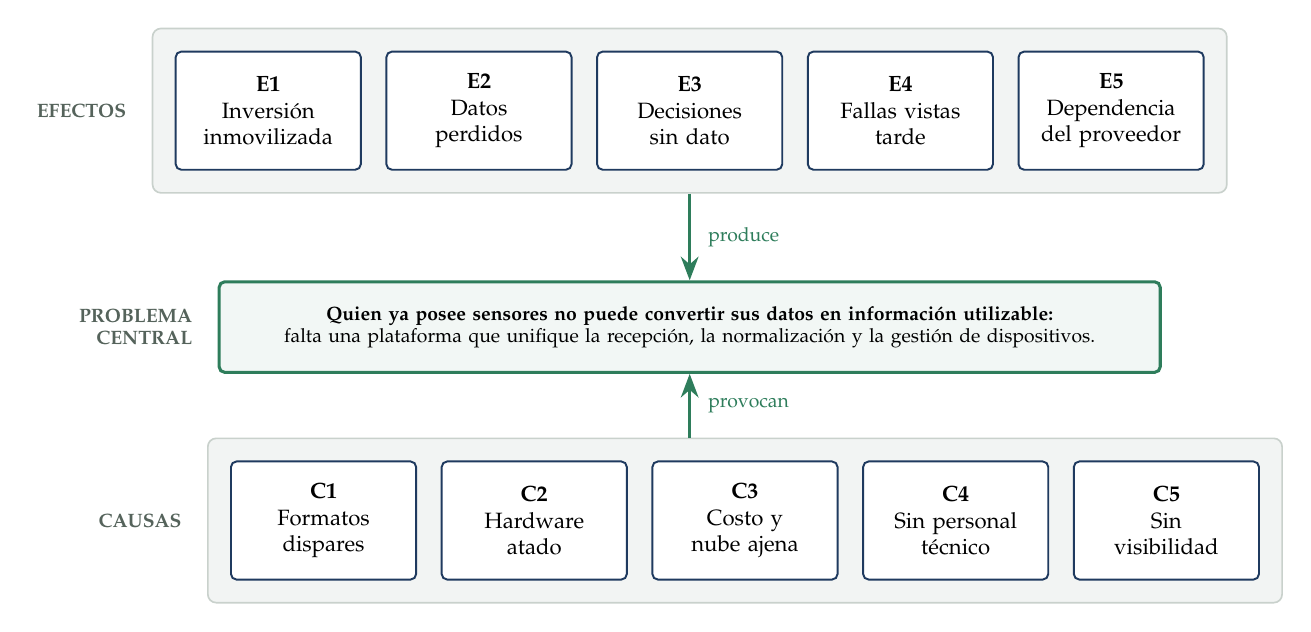
\begin{tikzpicture}[font=\scriptsize,
  cuadro/.style={caja, text width=2.0cm, minimum height=1.5cm, align=center}]

% ---- EFECTOS ----
\node[cuadro] (e1) {\textbf{E1}\\ Inversión\\ inmovilizada};
\node[cuadro, right=3mm of e1] (e2) {\textbf{E2}\\ Datos\\ perdidos};
\node[cuadro, right=3mm of e2] (e3) {\textbf{E3}\\ Decisiones\\ sin dato};
\node[cuadro, right=3mm of e3] (e4) {\textbf{E4}\\ Fallas vistas\\ tarde};
\node[cuadro, right=3mm of e4] (e5) {\textbf{E5}\\ Dependencia\\ del proveedor};
\begin{scope}[on background layer]
\node[grupo, fit=(e1)(e5)] (gefectos) {};
\end{scope}
\node[etiqueta, left=2mm of gefectos] {EFECTOS};

% ---- PROBLEMA CENTRAL ----
\node[cajaacento, below=11mm of gefectos, text width=11.6cm, minimum height=1.15cm,
      fill=verdeacento!6, font=\scriptsize, align=center] (prob)
  {\textbf{Quien ya posee sensores no puede convertir sus datos en información utilizable:}\\
   falta una plataforma que unifique la recepción, la normalización y la gestión de dispositivos.};
\node[etiqueta, left=2mm of prob] {PROBLEMA\\CENTRAL};

% ---- CAUSAS (con apodo memorizable) ----
\node[cuadro, below=11mm of prob, xshift=-4.65cm] (c1) {\textbf{C1}\\ Formatos\\ dispares};
\node[cuadro, right=3mm of c1] (c2) {\textbf{C2}\\ Hardware\\ atado};
\node[cuadro, right=3mm of c2] (c3) {\textbf{C3}\\ Costo y\\ nube ajena};
\node[cuadro, right=3mm of c3] (c4) {\textbf{C4}\\ Sin personal\\ técnico};
\node[cuadro, right=3mm of c4] (c5) {\textbf{C5}\\ Sin\\ visibilidad};
\begin{scope}[on background layer]
\node[grupo, fit=(c1)(c5)] (gcausas) {};
\end{scope}
\node[etiqueta, left=2mm of gcausas] {CAUSAS};

% ---- flechas perfectamente verticales, ancladas al centro del problema ----
\draw[flechagruesa] (prob.south |- gcausas.north) -- node[nota, right=1mm] {provocan} (prob.south);
\draw[flechagruesa] (prob.north |- gefectos.south) -- node[nota, right=1mm] {produce} (prob.north);
\end{tikzpicture}}
\caption{Árbol de problemas. Las cinco causas —C1 formatos dispares, C2 hardware atado, C3 costo y
nube ajena, C4 sin personal técnico, C5 sin visibilidad— provocan el problema central, que produce
los cinco efectos.}
\label{fig:arbol}
\end{figure}


\textbf{Evidencia.} La literatura identifica la fragmentación de protocolos y formatos como uno de los
desafíos centrales del Internet de las Cosas \parencite{alfuqaha2015} y documenta que la falta de
interoperabilidad y la dependencia de proveedor impiden su adopción a gran escala \parencite{noura2019},
lo que sustenta C1, C2 y C3. La evidencia directa de la Facultad ---necesidades, incidentes y uso
previsto de los datos--- se está levantando por entrevista (sección~\ref{sec:retro}).

\textbf{Organización destinataria y alcance.} La Universidad Católica de Temuco es la dueña del
problema; el caso de validación es el Campus Dr.\ Luis Rivas del Canto, sede de la Facultad de
Ingeniería. El trabajo abarca el sistema integrado, desde que un dispositivo IoT se registra hasta que
sus datos se muestran en el dashboard, incluido el diseño de la red por la que esos datos viajan desde
el sitio hasta el servidor. Los dispositivos y su radio no son parte de este trabajo. Quedan fuera la
fabricación de dispositivos y la analítica predictiva.

\section{Estado del arte}
\label{sec:estado-arte}

Hoy existen sistemas integrados de código abierto para registrar, gestionar y monitorear dispositivos
IoT, como OpenRemote, Magistrala y ThingsBoard; este último cambió de licencia en septiembre de 2026.
Existen además soluciones atadas a su propio hardware o a su servicio, como Milesight IoT Cloud o la
chilena Energetika, y plataformas comerciales en la nube, como Ubidots y TagoIO.

OpenRemote, bajo licencia AGPL~3.0 \parencite{openremotelicencia}, es el más completo de los abiertos:
paneles, reglas, alarmas, notificaciones por correo y al celular, llamadas a sistemas externos y mapa,
e integra redes LoRaWAN a través de ChirpStack; su instalación central exige además un servidor de
identidad, Keycloak \parencite{openremotedocs}. Magistrala libera su núcleo bajo Apache~2.0
\parencite{magistralalicencia}, pero deja los paneles, las alarmas, el motor de reglas y los reportes
fuera de su edición comunitaria \parencite{magistraladocs}. ThingsBoard, el más difundido, distribuye
desde su versión~4.4 su código bajo la \emph{Business Source License}, que permite el uso gratuito
con condiciones ---para una institución educativa, hasta 1\,000 dispositivos--- \parencite{thingsboardbusl};
la versión~4.3 sigue en Apache~2.0 \parencite{thingsboardlicencia43}. Su guía de instalación pide
4\,GB de memoria para pruebas y 8\,GB para una producción pequeña \parencite{thingsboardinstalacion}.

Milesight IoT Cloud acepta solo productos Milesight conectados a través de sus propias pasarelas, no
ofrece una API hacia otras plataformas y permite descargar los datos en CSV de a tres meses
\parencite{milesightfaq}; su plan gratuito admite 10 dispositivos y 2 paneles \parencite{milesightcloud}.
Energetika ofrece en Chile una plataforma propia, desarrollada y operada por la empresa, que trabaja
con los sensores que el cliente ya tiene \parencite{energetikaiotify}.

Ubidots y TagoIO aceptan equipos que no están en su catálogo \parencite{ubidotsdispositivos,tagodecodificador},
pero alojan los datos en servidores del proveedor, en Estados Unidos o Europa
\parencite{ubidotsseguridad,tagoapi}, con planes gratuitos de 3 y 5 dispositivos; el de Ubidots, solo
para uso no comercial y con un mes de retención \parencite{ubidotsstem,tagoprecios}.

Cada grupo resuelve una parte del problema y deja otra: las soluciones del fabricante atan los datos
a su hardware; las nubes comerciales limitan los dispositivos y guardan los datos fuera de la
institución; y las abiertas, que se instalan en un servidor propio, exigen componentes adicionales,
reservan funciones a su edición de pago o condicionan su uso. Este trabajo se ubica en el grupo de
código abierto, como prototipo: no compite en amplitud de funciones con OpenRemote o ThingsBoard.
Busca otra cosa: que el personal no técnico de una facultad registre y vigile sus dispositivos y deje
sus datos listos para investigación, exportables en formato abierto, con independencia del fabricante
y en la propia institución.

\section{Objetivos}
\label{sec:objetivos}
\subsection{Objetivo general}
\begin{itemize}
\item Desarrollar una plataforma web para el registro, monitoreo y gestión de datos de sensores,
que reciba las tramas de distintos sensores a través de TCP/IP, las normalice a un modelo interno
único, almacene las mediciones como series de tiempo, supervise el estado de cada dispositivo y
presente la información en un panel de control, validada sobre un caso de uso real en el Campus
Dr. Luis Rivas del Canto de la Universidad Católica de Temuco al término del semestre académico 2026.
\end{itemize}

\subsection{Objetivos específicos}
\begin{itemize}
\item \textbf{OE1} — Caracterizar la situación de gestión de datos de sensores en la organización
destinataria, mediante revisión de literatura, análisis de la oferta existente y al menos dos entrevistas
semiestructuradas documentadas (participantes, necesidades, prioridades), para validar un catálogo
de requerimientos trazable a las causas del problema, al 30 de octubre de 2026.
\item \textbf{OE2} — Evaluar y seleccionar el mecanismo de transporte y el formato de trama, y
especificar el contrato de entrada con sus adaptadores y política de cuarentena, mediante matrices
de criterios ponderados, para obtener el documento de especificación de la capa de recepción, al 2
de octubre de 2026.
\item \textbf{OE3} — Diseñar la arquitectura de la plataforma, su modelo de datos y su despliegue
con costo cuantificado, mediante la fase \emph{Design} de PPDIOO y la comparación de al menos tres
alternativas de alojamiento, para obtener los diagramas, el modelo y la recomendación justificada,
al 2 de octubre de 2026.
\item \textbf{OE4} — Implementar la plataforma, mediante desarrollo incremental, para obtener
primero el \textbf{núcleo mínimo demostrable} —recepción por MQTT, normalización, supervisión de
caída y consulta básica— con un sensor real de extremo a extremo al 30 de octubre de 2026, y luego
la entrada HTTP, las alertas y el panel de control al 4 de diciembre de 2026.
\item \textbf{OE5} — Validar la plataforma en un servidor de recursos modestos, mediante pruebas
funcionales, de carga y de recuperación, para obtener un informe de validación contra los umbrales
de los requerimientos no funcionales —al menos 15 casos de prueba con el 90\,\% aprobados; 50
mensajes por segundo sin pérdida; latencia de recepción a consulta de 2 segundos o menos en el
percentil 95; caída detectada en a lo más dos intervalos de reporte; recuperación automática sin
perder mensajes confirmados; disponibilidad de la recepción del 99\,\% o más en una ventana continua
de 72 horas; memoria total de 2\,GB o menos—, al 4 de diciembre de 2026.
\end{itemize}

El cuadro~\ref{tab:trazabilidad} resume el producto verificable de cada objetivo y su trazabilidad;
los hitos y metas numéricas están en el repositorio y en el capítulo~\ref{cap:metodologia}.

\begin{table}[H]
\centering\footnotesize
\begin{tablaseg}
\begin{tabular}{@{}L{2.9cm}L{3.5cm}L{1.9cm}L{1.3cm}L{2.2cm}C{0.9cm}@{}}
\toprule
\textbf{Objetivo} & \textbf{Producto verificable} & \textbf{Causas} & \textbf{Efectos} & \textbf{Fase PPDIOO} & \textbf{Etapa} \\
\midrule
OE1 Caracterizar & Catálogo de requerimientos con fuente por ítem (anexo~\ref{anx:requerimientos}); registros de entrevista & C4 (diagnostica C1--C5) & E1, E3 & Prepare & 1, 3 \\
OE2 Contrato de recepción & Especificación del contrato: tópico, SenML, adaptadores, cuarentena (cap.~\ref{cap:especificacion}) & \textbf{C1} & E2, E5 & Plan, Design & 2 \\
OE3 Arquitectura y despliegue & Vistas C4, ER y UML; recomendación de alojamiento con costo (cap.~\ref{cap:diseno}) & C2, C3, C5 & E1, E4, E5 & Design, Plan & 2 \\
OE4 Implementar & Prototipo en repositorio: núcleo mínimo y luego segundo nivel & C1, C2, C4 & E1--E3 & Implement & 3, 4 \\
OE5 Validar & Informe de validación contra los umbrales & C5 & E4 & Operate, Optimize & 4 \\
\bottomrule
\end{tabular}
\end{tablaseg}
\caption{Matriz de trazabilidad: producto verificable de cada objetivo, causas y efectos que ataca,
fase y etapa. Las cinco causas y los cinco efectos quedan cubiertos por al menos un objetivo.}
\label{tab:trazabilidad}
\end{table}

\section{Autoría y licenciamiento}

Este trabajo, su documentación y el código son de \textbf{autoría de Vicente Ricardo Ramírez Oñate};
la universidad es la organización destinataria del producto, no la titular de la obra. La licencia
de publicación se decidirá antes de liberar el resultado, evaluando opciones que permitan el uso
abierto e impidan el aprovechamiento comercial por terceros sin acuerdo con el autor.

\section{Estructura del documento}

Antecedentes técnicos (cap.~\ref{cap:antecedentes}); requerimientos y evaluaciones
(cap.~\ref{cap:especificacion}); diseño desde varias vistas, nuevo en esta etapa
(cap.~\ref{cap:diseno}); metodología, seguimiento y retroalimentación incorporada
(cap.~\ref{cap:metodologia}); anexos con el catálogo, el backlog, las evaluaciones, figuras
complementarias y el camino descartado.

\chapter{Antecedentes}
\label{cap:antecedentes}

\section{Los protocolos se apilan, no compiten}

Al enumerar «WiFi», «LoRaWAN» y «Contact ID» parece tratarse de alternativas entre las cuales elegir.
Operan en niveles distintos: la capa de \textbf{aplicación} define qué significa el mensaje (Contact
ID, JSON, SenML); la de \textbf{red y transporte}, cómo llega (IP, TCP/UDP, LoRaWAN, DC-09); la
\textbf{física}, cómo viajan los bits (WiFi 802.11, LoRa, cable). La independencia entre niveles es lo
que hace posible la propuesta: \textbf{el mismo mensaje Contact ID llega por radio LoRa, por WiFi o por
cable, y la plataforma lo interpreta de forma idéntica} (figura~\ref{fig:pila}).

\begin{figure}[H]
\centering
\resizebox{0.86\linewidth}{!}{%
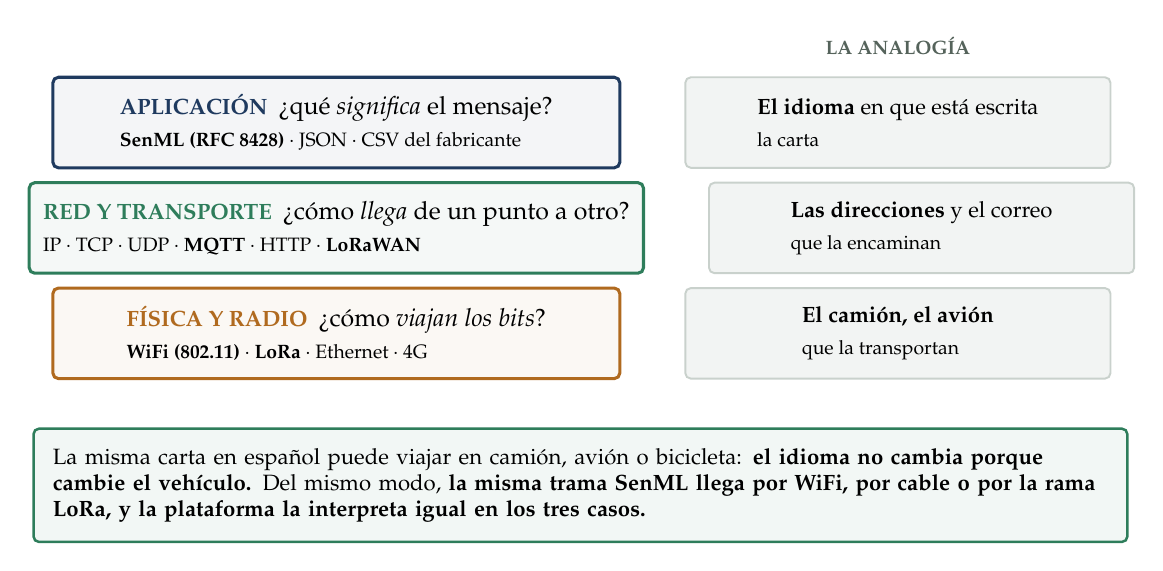
\begin{tikzpicture}[font=\footnotesize]

\def\w{7.2}   % ancho de las cajas de capa
\def\h{1.15}  % alto de cada capa

% ---- capas ----
\node[caja, minimum width=\w cm, minimum height=\h cm, align=left,
      draw=azuloscuro, line width=1.1pt, fill=azuloscuro!5] (app) at (0,0)
  {\textbf{\color{azuloscuro}APLICACIÓN}\ \ \small ¿qué \emph{significa} el mensaje?\\[2pt]
   \scriptsize \textbf{SenML (RFC 8428)} · JSON · CSV del fabricante};

\node[caja, minimum width=\w cm, minimum height=\h cm, align=left,
      draw=verdeacento, line width=1.1pt, fill=verdeacento!5, below=1.5mm of app] (red)
  {\textbf{\color{verdeacento}RED Y TRANSPORTE}\ \ \small ¿cómo \emph{llega} de un punto a otro?\\[2pt]
   \scriptsize IP · TCP · UDP · \textbf{MQTT} · HTTP · \textbf{LoRaWAN}};

\node[caja, minimum width=\w cm, minimum height=\h cm, align=left,
      draw=ambar, line width=1.1pt, fill=ambar!5, below=1.5mm of red] (fis)
  {\textbf{\color{ambar}FÍSICA Y RADIO}\ \ \small ¿cómo \emph{viajan los bits}?\\[2pt]
   \scriptsize \textbf{WiFi (802.11)} · \textbf{LoRa} · Ethernet · 4G};

% ---- analogia de la carta ----
\node[caja, minimum width=5.4cm, minimum height=\h cm, align=left, right=8mm of app,
      draw=grislinea, fill=grisclaro] (a1)
  {\textbf{El idioma} en que está escrita\\[2pt]\scriptsize la carta};
\node[caja, minimum width=5.4cm, minimum height=\h cm, align=left, right=8mm of red,
      draw=grislinea, fill=grisclaro] (a2)
  {\textbf{Las direcciones} y el correo\\[2pt]\scriptsize que la encaminan};
\node[caja, minimum width=5.4cm, minimum height=\h cm, align=left, right=8mm of fis,
      draw=grislinea, fill=grisclaro] (a3)
  {\textbf{El camión, el avión}\\[2pt]\scriptsize que la transportan};

\node[nota, above=1.5mm of a1, font=\scriptsize\bfseries\color{gristexto}] {LA ANALOGÍA};

% ---- conclusion ----
\node[notaclave, below=6mm of fis.south, anchor=north, text width=13.4cm, xshift=3.1cm,
      fill=verdeacento!6, font=\footnotesize]
  {La misma carta en español puede viajar en camión, avión o bicicleta: \textbf{el idioma no cambia
   porque cambie el vehículo.} Del mismo modo, \textbf{la misma trama SenML llega por WiFi, por cable o
   por la rama LoRa, y la plataforma la interpreta igual en los tres casos.}};

\end{tikzpicture}}
\caption{Los protocolos se apilan, no compiten. Cada nivel responde una pregunta distinta, y la
elección en un nivel no condiciona la de los otros.}
\label{fig:pila}
\end{figure}


\section{Tecnologías de radio: LoRa y LoRaWAN}

\textbf{LoRa} es la técnica de modulación de radio (capa física, patente Semtech); \textbf{LoRaWAN} es
el protocolo de red abierto construido sobre ella: registro de dispositivos, cifrado AES-128 de extremo
a extremo y entrega al servidor \parencite{rp002}. La analogía exacta: LoRa es a LoRaWAN lo que 802.11
es a TCP/IP. Chile emplea la banda libre de 915--928\,MHz (Resolución 737 de Subtel
\parencite{lorachile}).

LoRa intercambia velocidad por alcance y autonomía: 0,3--27\,kbps y payloads de 11 a 53 bytes según la
tasa de datos, a cambio de 2--15\,km de alcance y años de batería. Su patrón de uso —lecturas breves y
avisos— coincide con el de los sensores de este trabajo. La cadena completa es nodo $\rightarrow$
gateway (traductor sin claves) $\rightarrow$ servidor de red ChirpStack (descifra, deduplica,
administra, reporta RSSI/SNR y publica en MQTT) $\rightarrow$ plataforma (figura~\ref{fig:lorawan}).

\begin{figure}[htbp]
\centering
\resizebox{\linewidth}{!}{%
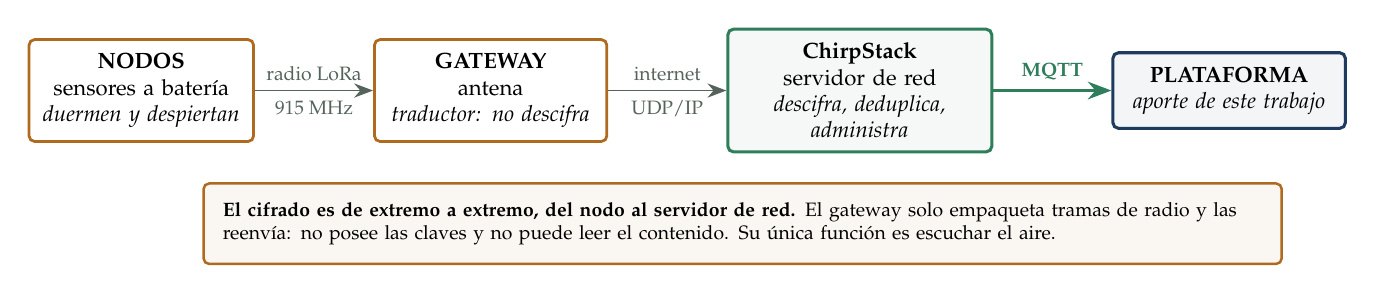
\begin{tikzpicture}[font=\scriptsize]

\node[caja, text width=2.5cm, align=center, draw=ambar, line width=1pt] (nodos)
  {\textbf{NODOS}\\ sensores a batería\\ \emph{duermen y despiertan}};

\node[caja, text width=2.6cm, align=center, right=1.5cm of nodos, draw=ambar, line width=1pt] (gw)
  {\textbf{GATEWAY}\\ antena\\ \emph{traductor: no descifra}};

\node[caja, text width=3.0cm, align=center, right=1.5cm of gw, draw=verdeacento, line width=1.1pt,
      fill=verdeacento!5] (cs)
  {\textbf{ChirpStack}\\ servidor de red\\ \emph{descifra, deduplica, administra}};

\node[caja, text width=2.6cm, align=center, right=1.5cm of cs, draw=azuloscuro, line width=1.1pt,
      fill=azuloscuro!5] (plat)
  {\textbf{PLATAFORMA}\\ \emph{aporte de este trabajo}};

\draw[flecha] (nodos) -- node[nota, above, font=\scriptsize] {radio LoRa} node[nota, below, font=\scriptsize] {915 MHz} (gw);
\draw[flecha] (gw) -- node[nota, above, font=\scriptsize] {internet} node[nota, below, font=\scriptsize] {UDP/IP} (cs);
\draw[flechagruesa] (cs) -- node[nota, above, font=\scriptsize\bfseries\color{verdeacento}] {MQTT} (plat);

\node[notaaviso, below=5mm of gw.south, anchor=north, text width=13.2cm, xshift=3.2cm,
      fill=ambar!6, font=\scriptsize]
  {\textbf{El cifrado es de extremo a extremo, del nodo al servidor de red.} El gateway solo empaqueta
   tramas de radio y las reenvía: no posee las claves y no puede leer el contenido. Su única función es
   escuchar el aire.};

\end{tikzpicture}}
\caption{Cadena de una red LoRaWAN y ubicación del aporte de este trabajo.}
\label{fig:lorawan}
\end{figure}


\section{Mensajería MQTT}

MQTT aplica el patrón publicar/suscribir a través de un \emph{broker} (figura~\ref{fig:mqtt}). Dos
propiedades resultan determinantes: (1) \textbf{el dispositivo inicia la conexión saliente}, lo que
evita abrir puertos hacia los sensores y funciona tras NAT y cortafuegos —materializa el requerimiento
RNF-10—; (2) el mecanismo \emph{Last Will and Testament} notifica automáticamente la desconexión
abrupta de un cliente, lo que se traduce directamente al código 381 de Contact ID sin lógica adicional.

\begin{figure}[H]
\centering
\resizebox{0.8\linewidth}{!}{%
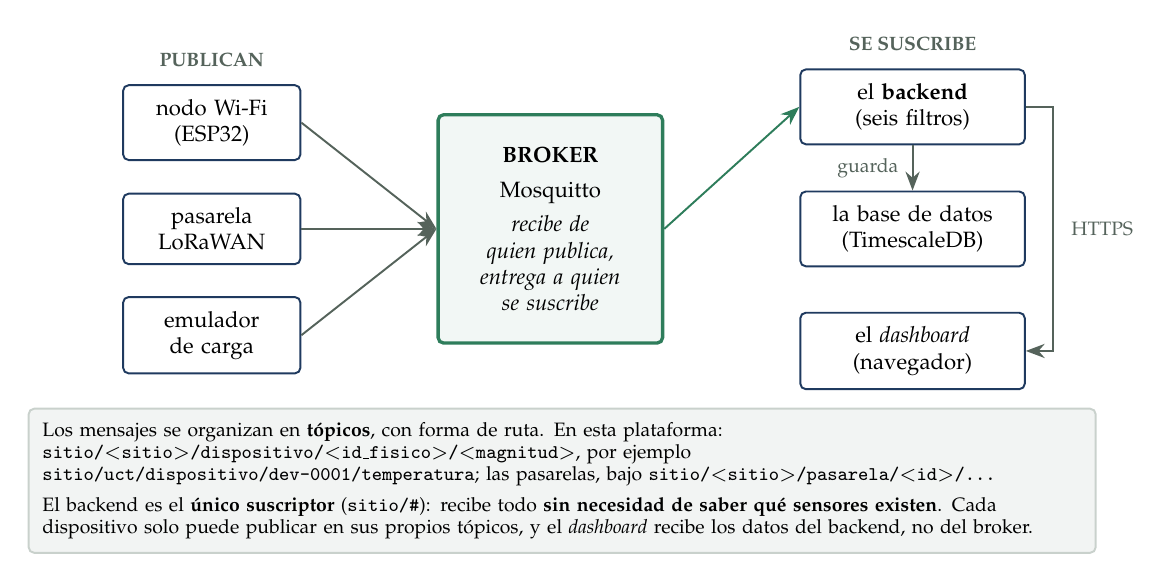
\begin{tikzpicture}[font=\scriptsize]

\node[caja, text width=1.9cm] (s1) at (0,1.35) {nodo Wi-Fi\\(ESP32)};
\node[caja, text width=1.9cm] (s2) at (0,0)    {pasarela LoRaWAN};
\node[caja, text width=1.9cm] (s3) at (0,-1.35){emulador de carga};

\node[caja, text width=2.5cm, align=center, draw=verdeacento, line width=1.2pt,
      fill=verdeacento!6, minimum height=2.9cm] (br) at (4.3,0)
  {\textbf{BROKER}\\[3pt] Mosquitto\\[3pt] \emph{recibe de quien publica,\\ entrega a quien se suscribe}};

\node[caja, text width=2.5cm] (c1) at (8.9,1.55) {el \textbf{backend}\\(seis filtros)};
\node[caja, text width=2.5cm] (c2) at (8.9,0)    {la base de datos\\(TimescaleDB)};
\node[caja, text width=2.5cm] (c3) at (8.9,-1.55){el \emph{dashboard}\\(navegador)};

\foreach \s in {s1,s2,s3} \draw[flecha] (\s.east) -- (br.west);
\draw[flecha, color=verdeacento] (br.east) -- (c1.west);
\draw[flecha] (c1.south) -- node[nota, left=0.5mm]{guarda} (c2.north);
\draw[flecha] (c1.east) -- ++(0.35,0) |- node[nota, pos=0.25, right=1mm]{HTTPS} (c3.east);

\node[nota, above=1mm of s1, font=\scriptsize\bfseries\color{gristexto}] {PUBLICAN};
\node[nota, above=1mm of c1, font=\scriptsize\bfseries\color{gristexto}] {SE SUSCRIBE};

\node[caja, below=8mm of br.south, anchor=north, text width=13.2cm, xshift=0.15cm,
      draw=grislinea, fill=grisclaro, font=\scriptsize, align=left]
  {Los mensajes se organizan en \textbf{tópicos}, con forma de ruta. En esta plataforma:
   \texttt{sitio/\textless sitio\textgreater/dispositivo/\textless id\_fisico\textgreater/\textless magnitud\textgreater}, por ejemplo \texttt{sitio/uct/dispositivo/dev-0001/temperatura}; las pasarelas, bajo \texttt{sitio/\textless sitio\textgreater/pasarela/\textless id\textgreater/…}\\[3pt]
   El backend es el \textbf{único suscriptor} (\texttt{sitio/\#}): recibe todo \textbf{sin necesidad de saber qué sensores
   existen}. Cada dispositivo solo puede publicar en sus propios tópicos, y el \emph{dashboard} recibe los datos del backend, no del broker.};

\end{tikzpicture}}
\caption{Patrón publicar/suscribir de MQTT en este sistema. El desacoplamiento entre emisores y receptor es lo que
permite sumar dispositivos sin tocar el backend.}
\label{fig:mqtt}
\end{figure}


\section{El protocolo Contact ID (SIA DC-05)}

Contact ID es el protocolo de reporte de eventos de la industria de alarmas, formalizado por la
Security Industry Association como estándar DC-05 \parencite{siadc05}. Tres estándares SIA se apilan:
\textbf{DC-05} define el formato del mensaje; DC-03 \parencite{siadc03} es un formato alternativo más
expresivo; \textbf{DC-09} \parencite{siadc09} transporta cualquiera de los dos sobre IP con cifrado
AES opcional y, en su revisión 2026, rotación de claves y auto-comisionamiento.

El mensaje es una secuencia de \textbf{16 dígitos} (figura~\ref{fig:mensaje}): cuenta (ACCT), tipo
(MT=18), calificador (\texttt{Q}: 1 abre una condición, 3 la cierra —una máquina de estados nativa—),
código de evento (XYZ), partición (GG), zona (CCC) y suma de comprobación módulo 15. El alfabeto tiene
15 símbolos porque el transporte original fue DTMF: tonos telefónicos, donde el cero vale diez.

\begin{figure}[htbp]
\centering
\resizebox{\linewidth}{!}{%
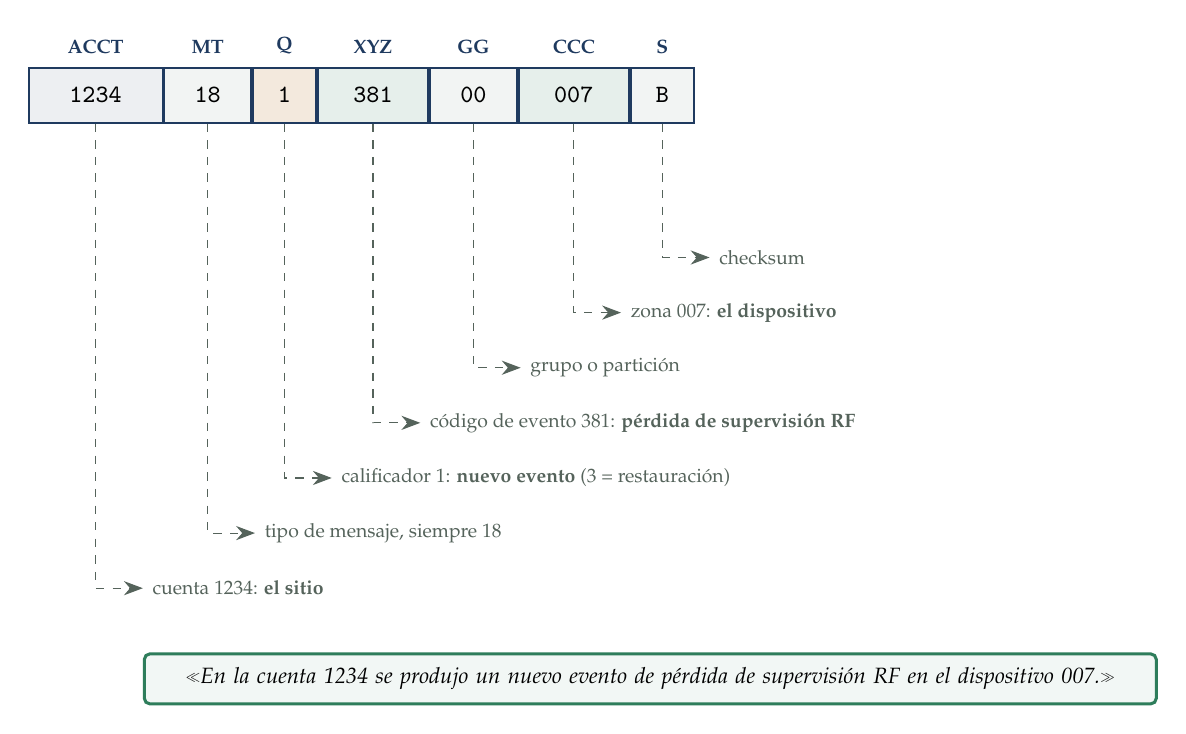
\begin{tikzpicture}

% ---- campos del mensaje ----
\node[campo, minimum width=17mm, fill=azuloscuro!8] (acct) {1234};
\node[campo, minimum width=11mm, right=0pt of acct, fill=grisclaro] (mt) {18};
\node[campo, minimum width=8mm,  right=0pt of mt,   fill=ambar!15]  (q)   {1};
\node[campo, minimum width=14mm, right=0pt of q,    fill=verdeacento!12] (xyz) {381};
\node[campo, minimum width=11mm, right=0pt of xyz,  fill=grisclaro] (gg)  {00};
\node[campo, minimum width=14mm, right=0pt of gg,   fill=verdeacento!12] (ccc) {007};
\node[campo, minimum width=8mm,  right=0pt of ccc,  fill=grisclaro] (s)   {B};

% ---- nombres de campo encima ----
\foreach \n/\l in {acct/ACCT, mt/MT, q/Q, xyz/XYZ, gg/GG, ccc/CCC, s/S}
  \node[font=\scriptsize\bfseries\color{azuloscuro}, above=1pt of \n] {\l};

% ---- descripciones debajo, escalonadas ----
\node[nota, below=17mm of s.south, xshift=6mm, anchor=west]   (ds)   {checksum};
\node[nota, below=24mm of ccc.south, xshift=6mm, anchor=west] (dccc) {zona 007: \textbf{el dispositivo}};
\node[nota, below=31mm of gg.south, xshift=6mm, anchor=west]  (dgg)  {grupo o partición};
\node[nota, below=38mm of xyz.south, xshift=6mm, anchor=west] (dxyz) {código de evento 381: \textbf{pérdida de supervisión RF}};
\node[nota, below=45mm of q.south, xshift=6mm, anchor=west]    (dq)   {calificador 1: \textbf{nuevo evento} (3 = restauración)};
\node[nota, below=52mm of mt.south, xshift=6mm, anchor=west]  (dmt)  {tipo de mensaje, siempre 18};
\node[nota, below=59mm of acct.south, xshift=6mm, anchor=west](dacct){cuenta 1234: \textbf{el sitio}};

\foreach \c/\d in {s/ds, ccc/dccc, gg/dgg, xyz/dxyz, q/dq, mt/dmt, acct/dacct} {
  \draw[flecha, dashed, line width=0.4pt] (\c.south) |- (\d.west);
}

% ---- lectura ----
\node[cajaacento, below=6mm of dacct.south west, anchor=north west, text width=12.5cm,
      fill=verdeacento!6, font=\footnotesize\itshape]
  {«En la cuenta 1234 se produjo un nuevo evento de pérdida de supervisión RF
    en el dispositivo 007.»};

\end{tikzpicture}}
\caption{Estructura del mensaje Contact ID: 16 dígitos distribuidos en siete campos.}
\label{fig:mensaje}
\end{figure}


La transmisión original incluía el \emph{kissoff}: la receptora confirma solo si la suma de
comprobación es válida, y el panel reintenta en su ausencia —confirmación a nivel de aplicación que
este trabajo conserva—. La «comunicación celular» de las alarmas modernas es un cambio de transporte,
no de protocolo (figura~\ref{fig:alarmas}); el mensaje de 16 dígitos nació para caber en tonos sobre
una línea analógica, \textbf{y esa restricción de hace cuatro décadas es la que hoy lo hace apropiado
para LoRa}, un canal igualmente estrecho.

\begin{figure}[htbp]
\centering
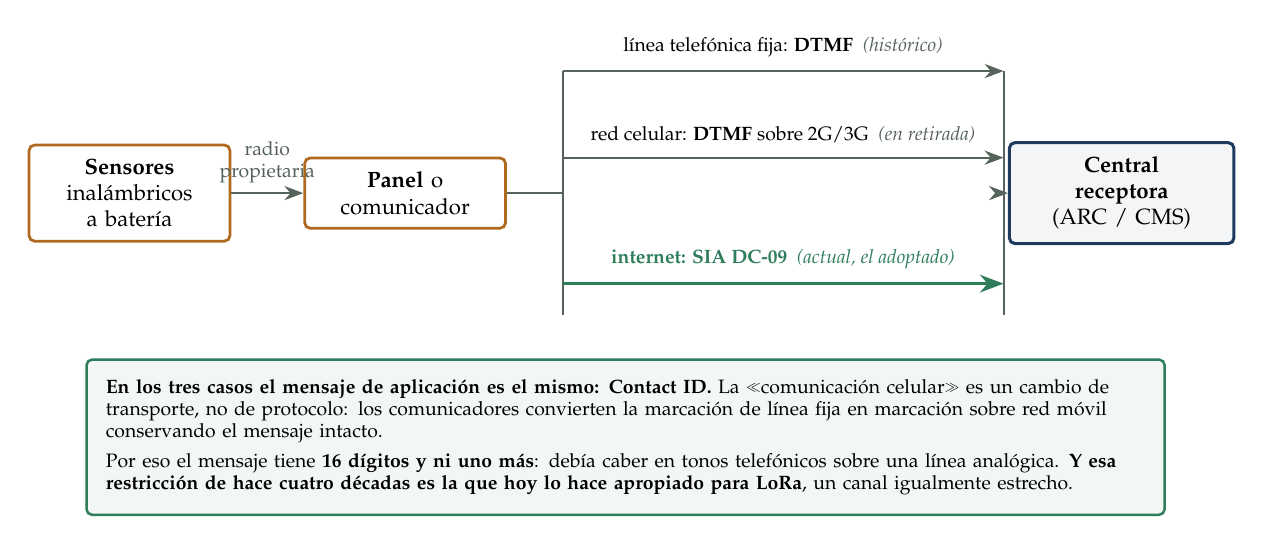
\begin{tikzpicture}[font=\scriptsize]

% ---- sensores y panel ----
\node[caja, text width=2.2cm, align=center, draw=ambar, line width=1pt] (sens) at (0,0)
  {\textbf{Sensores}\\ inalámbricos\\ a batería};

\node[caja, text width=2.2cm, align=center, draw=ambar, line width=1pt] (panel) at (3.5,0)
  {\textbf{Panel} o\\ comunicador};

\draw[flecha] (sens) -- node[nota, above, font=\scriptsize, align=center] {radio\\propietaria} (panel);

% ---- central receptora ----
\node[caja, text width=2.5cm, align=center, draw=azuloscuro, line width=1.1pt,
      fill=azuloscuro!5] (arc) at (12.6,0)
  {\textbf{Central}\\ \textbf{receptora}\\ (ARC / CMS)};

% ---- punto de bifurcacion: el panel elige transporte ----
\coordinate (bif) at (5.5,0);
\draw[line width=0.7pt, color=gristexto] (panel.east) -- (bif);
\draw[line width=0.7pt, color=gristexto] (5.5,1.55) -- (5.5,-1.55);

\coordinate (conv) at (11.1,0);
\draw[line width=0.7pt, color=gristexto] (11.1,1.55) -- (11.1,-1.55);
\draw[flecha] (conv) -- (arc.west);

% ---- las tres generaciones, con etiqueta centrada en el tramo ----
\draw[flecha] (5.5,1.55) -- (11.1,1.55);
\node[nota, above=0.6mm of {(8.3,1.55)}, font=\scriptsize]
  {línea telefónica fija: \textbf{DTMF}\ \ \textcolor{gristexto}{\itshape (histórico)}};

\draw[flecha] (5.5,0.45) -- (11.1,0.45);
\node[nota, above=0.6mm of {(8.3,0.45)}, font=\scriptsize]
  {red celular: \textbf{DTMF} sobre 2G/3G\ \ \textcolor{gristexto}{\itshape (en retirada)}};

\draw[flechagruesa] (5.5,-1.15) -- (11.1,-1.15);
\node[nota, above=0.6mm of {(8.3,-1.15)}, font=\scriptsize\color{verdeacento}]
  {\textbf{internet: SIA DC-09}\ \ \itshape (actual, el adoptado)};

% ---- nota final ----
\node[notaclave, text width=13.2cm, fill=verdeacento!6, font=\scriptsize, align=left]
      at (6.3,-3.1)
  {\textbf{En los tres casos el mensaje de aplicación es el mismo: Contact ID.} La «comunicación
   celular» es un cambio de transporte, no de protocolo: los comunicadores convierten la marcación de
   línea fija en marcación sobre red móvil conservando el mensaje intacto.\\[3pt]
   Por eso el mensaje tiene \textbf{16 dígitos y ni uno más}: debía caber en tonos telefónicos sobre una
   línea analógica. \textbf{Y esa restricción de hace cuatro décadas es la que hoy lo hace apropiado
   para LoRa}, un canal igualmente estrecho.};

\end{tikzpicture}
\caption{Cadena de comunicación de una alarma monitoreada. El formato del mensaje se conserva a través
de tres generaciones de transporte.}
\label{fig:alarmas}
\end{figure}


Su vocabulario incluye los eventos de salud de dispositivos inalámbricos que este trabajo necesita:
pérdida de supervisión RF (381), batería baja (384), interferencia (344), pruebas periódicas (602/603),
además de condiciones medibles (temperatura 158/159, agua 154, accesos 134/400)
\parencite{contactidcodes}.

\section{Persistencia de series de tiempo}

Los datos de sensores son voluminosos y siempre temporales: cincuenta sensores cada cinco minutos
generan cinco millones de registros anuales. Se emplea TimescaleDB, extensión de PostgreSQL que
conserva el modelo relacional y el SQL estándar, añadiendo particionado automático por tiempo,
agregación por intervalos y políticas de retención. La evaluación frente a alternativas está en la
sección~\ref{sec:infra}.

\chapter[Análisis de requerimientos]{Especificación: análisis de requerimientos}
\label{cap:especificacion}

\section{Metodología del levantamiento}

Cada requerimiento declara su fuente: \textbf{[PO]} solicitud de la organización destinataria
—«propietario del proyecto» en la terminología de la rúbrica— vía profesor guía; \textbf{[EM]}
estudio de mercado; \textbf{[BT]} base teórica (RFC 8428, ISO/IEC 25010 \parencite{iso25010}, SWEBOK
\parencite{swebok}); \textbf{[DP]} derivación del problema. \textbf{Brecha declarada:} falta la
fuente [ENT], entrevistas directas; su cierre es la acción prioritaria del período.

\section{Síntesis del catálogo}

Se catalogan \textbf{68 requerimientos}: 52 \textbf{funcionales} (RF: lo que el sistema debe
\emph{hacer}) en ocho módulos, y 16 \textbf{no funcionales} (RNF: cómo debe \emph{comportarse} —
rendimiento, seguridad, mantenibilidad) clasificados según
ISO/IEC 25010— con prioridad MoSCoW (49 \emph{Must}, 16 \emph{Should}, 3 \emph{Could}). El catálogo
completo está en el anexo~\ref{anx:requerimientos}.

\begin{table}[H]
\centering\footnotesize
\begin{tabular}{@{}cL{6.2cm}cL{3.2cm}@{}}
\toprule
\textbf{Módulo} & \textbf{Responsabilidad} & \textbf{Req.} & \textbf{Causas} \\
\midrule
M1 & Recepción multiprotocolo (MQTT, HTTP, adaptadores) & 10 & C1, C2 \\
M2 & Normalización al modelo interno (el pipeline) & 7 & C1, C5 \\
M3 & Registro y aprovisionamiento de dispositivos & 6 & C4, C5 \\
M4 & Supervisión de salud (¿quién dejó de reportar?) & 7 & \textbf{C5} \\
M5 & Persistencia y consulta de series de tiempo & 5 & C1, C3, C4 \\
M6 & Alertas y notificación & 4 & C5 \\
M7 & Seguridad, identidad y multi-tenencia & 7 & C1, C3, C4 \\
M8 & Panel de control (la vista, no el todo) & 6 & C1, C2, C4, C5 \\
\bottomrule
\end{tabular}
\caption{Módulos de la solución. El panel es uno de ocho módulos: la sustancia de ingeniería está en
M1--M7.}
\label{tab:modulos}
\end{table}

Requerimientos que anclan el trabajo al dominio de redes: \textbf{RNF-09} (dispositivos en segmento
de red separado), \textbf{RNF-10} (solo conexiones salientes desde los nodos), \textbf{RNF-12}
(añadir una vía de recepción no modifica el núcleo) y \textbf{RNF-16} (la trama nativa cumple SenML).
Y los que sustentan la diferenciación: \textbf{RF-04} (adaptadores por formato), \textbf{RF-24/27/30}
(supervisión de salud) y \textbf{RF-34} (exportación en formato abierto).

\section{Evaluación del mecanismo de transporte}
\label{sec:transporte}

Cinco alternativas sobre seis criterios. Los pesos derivan del problema: la plataforma debe saber
qué llegó y qué no (25\,\%), detectar dispositivos caídos (20\,\%, causa C5), exigir poco al nodo
(20\,\%, lo implementa el compañero), integrarse con poco esfuerzo al backend (15\,\%), pesar poco
por mensaje (10\,\%, la objeción a las cabeceras) y funcionar tras NAT sin abrir puertos (10\,\%,
RNF-10).

\begin{table}[H]
\centering\scriptsize\setlength{\tabcolsep}{2pt}
\begin{tabular}{@{}L{2.7cm}C{1.4cm}C{1.4cm}C{1.3cm}C{1.4cm}C{1.5cm}C{1.1cm}C{1.0cm}@{}}
\toprule
 & \textbf{Entrega confiable} & \textbf{Detecta caídos} & \textbf{Costo en nodo} & \textbf{Facilidad backend} & \textbf{Sobrecarga mensaje} & \textbf{Tras NAT} & \textbf{Total} \\
 & 25\,\% & 20\,\% & 20\,\% & 15\,\% & 10\,\% & 10\,\% & \\
\midrule
\textbf{MQTT} & \textbf{5} & \textbf{5} & 4 & \textbf{5} & \textbf{5} & \textbf{5} & \textbf{4,85} \\
HTTP/REST & 3 & 2 & 4 & \textbf{5} & 2 & \textbf{5} & 3,45 \\
CoAP & 3 & 2 & 4 & 2 & \textbf{5} & 4 & 3,05 \\
WebSocket & 2 & 3 & 3 & 3 & 4 & \textbf{5} & 3,05 \\
Socket TCP propio & 1 & 2 & \textbf{5} & 1 & \textbf{5} & \textbf{5} & 2,60 \\
\bottomrule
\end{tabular}
\caption{Evaluación del mecanismo de transporte (escala 1--5). Los pros y contras en palabras de
cada alternativa están en el anexo~\ref{anx:evaluacion}.}
\label{tab:transporte}
\end{table}

\textbf{Decisión:} MQTT como vía principal —QoS y \emph{Last Will} resuelven de fábrica la entrega
confiable y la detección de caída— y HTTP/REST como vía secundaria para integraciones. El navegador
nunca toca MQTT: consulta la API REST del backend. El socket TCP propio se descarta explícitamente:
lograría la mínima sobrecarga a costa de reinventar sesiones, confirmaciones y formato.

\section{Evaluación del formato de trama}

\begin{table}[H]
\centering\footnotesize
\begin{tabular}{@{}L{2.6cm}L{4.6cm}L{5.6cm}@{}}
\toprule
\textbf{Alternativa} & \textbf{A favor} & \textbf{En contra} \\
\midrule
JSON libre & Flexible, universal & \textbf{Reproduce la causa C1}: cada fuente con sus campos \\
\textbf{SenML (RFC 8428)} & Estándar IETF abierto; identidad, unidades y tiempo resueltos; legible & Algo más extenso que un JSON ad hoc \\
Binario propio & Mínimo peso & Indocumentado, difícil de depurar; solo se justifica en radio \\
CBOR & Compacto y estándar & Ilegible a ojo; librería adicional en el nodo \\
\bottomrule
\end{tabular}
\caption{Evaluación del formato de trama.}
\label{tab:formato}
\end{table}

\textbf{Decisión:} \textbf{SenML como contrato nativo}. Lo que no llegue en SenML entra mediante
\textbf{adaptadores por formato} (uno por formato de fuente, no por sensor); la trama malformada de
un dispositivo conocido va a \textbf{cuarentena} —cruda, con su motivo, sin contaminar las series—;
el dispositivo no registrado se \textbf{rechaza y se registra el intento}. Este es el mismo patrón
de entrada que aplica ThingsBoard con su formato propio \parencite{thingsboardmqtt}; la diferencia
es que aquí el contrato nativo es un estándar abierto.

\section{Arquitectura de recepción y frontera del trabajo}
\label{sec:frontera}

El aporte central es el \textbf{pipeline de tratamiento de tramas} (figura~\ref{fig:pipeline}):
seis filtros independientes y verificables por separado. La identificación de dispositivos combina
el \textbf{registro} (al dar de alta: identidad, tipo, ubicación, credencial) con la
\textbf{autoidentificación} de cada trama (el campo \texttt{bn}); el filtro de validación cruza
ambos.

\begin{figure}[H]
\centering
\resizebox{\linewidth}{!}{%
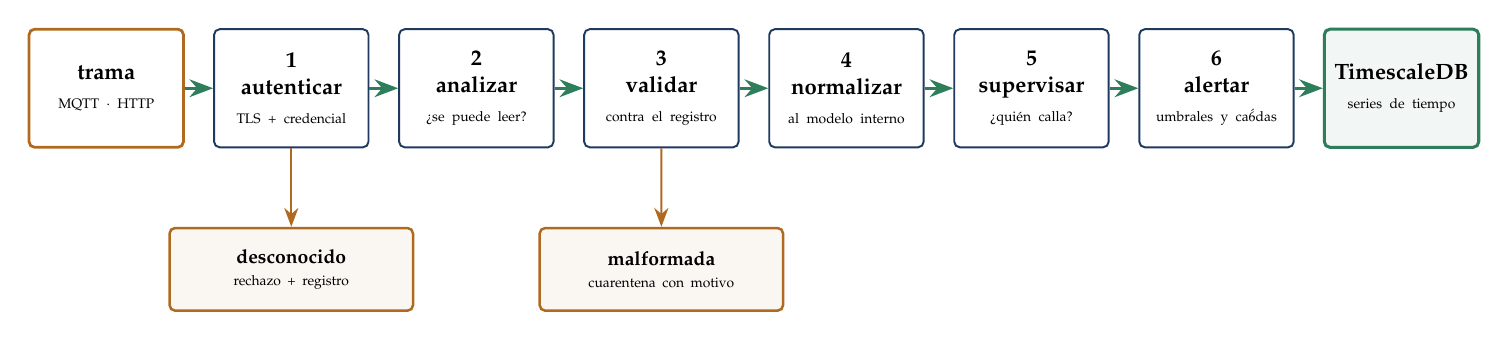
\begin{tikzpicture}[font=\scriptsize,
  filtro/.style={caja, text width=1.75cm, minimum height=1.5cm, align=center, inner sep=3pt}]

\node[filtro, draw=ambar, line width=1pt] (in) at (0,0) {\textbf{trama}\\[1pt]{\tiny MQTT · HTTP}};

\foreach \i/\nom/\det in {
  1/{autenticar}/{TLS + credencial},
  2/{analizar}/{¿se puede leer?},
  3/{validar}/{contra el registro},
  4/{normalizar}/{al modelo interno},
  5/{supervisar}/{¿quién calla?},
  6/{alertar}/{umbrales y caídas}}{
  \pgfmathsetmacro\x{\i*2.35}
  \node[filtro] (f\i) at (\x,0) {\textbf{\i}\\ \textbf{\nom}\\[1pt]{\tiny \det}};
}
\node[filtro, draw=verdeacento, line width=1.1pt, fill=verdeacento!6] (db) at (16.45,0)
  {\textbf{TimescaleDB}\\[1pt]{\tiny series de tiempo}};

\draw[flechagruesa] (in) -- (f1);
\foreach \i [evaluate=\i as \j using int(\i+1)] in {1,...,5} \draw[flechagruesa] (f\i) -- (f\j);
\draw[flechagruesa] (f6) -- (db);

% rechazos: caída vertical bajo su filtro
\node[notaaviso, text width=2.6cm, align=center, minimum height=1.05cm] (des) at (2.35,-2.3)
  {\textbf{desconocido}\\{\tiny rechazo + registro}};
\node[notaaviso, text width=2.6cm, align=center, minimum height=1.05cm] (cua) at (7.05,-2.3)
  {\textbf{malformada}\\{\tiny cuarentena con motivo}};
\draw[flecha, color=ambar] (f1.south) -- (des.north);
\draw[flecha, color=ambar] (f3.south) -- (cua.north);
\end{tikzpicture}}
\caption{El pipeline de tratamiento de tramas, aporte central del trabajo. Cada filtro es
independiente y verificable por separado; las dos salidas de rechazo preservan la evidencia sin
contaminar las series.}
\label{fig:pipeline}
\end{figure}


El despliegue completo corre como contenedores en un único servidor (figura~\ref{fig:despliegue}),
con reinicio automático ante fallas. \textbf{La frontera con el trabajo del compañero es el tópico
MQTT}: todo lo anterior (sensor, nodo, radio) es de él; todo lo posterior (broker, pipeline, base de
datos, API, panel), de este trabajo. Un \textbf{emulador de nodo} publica tramas en el mismo tópico,
de modo que la validación de la plataforma no depende del hardware ni de terceros.

\begin{figure}[htbp]
\centering
\resizebox{0.98\linewidth}{!}{%
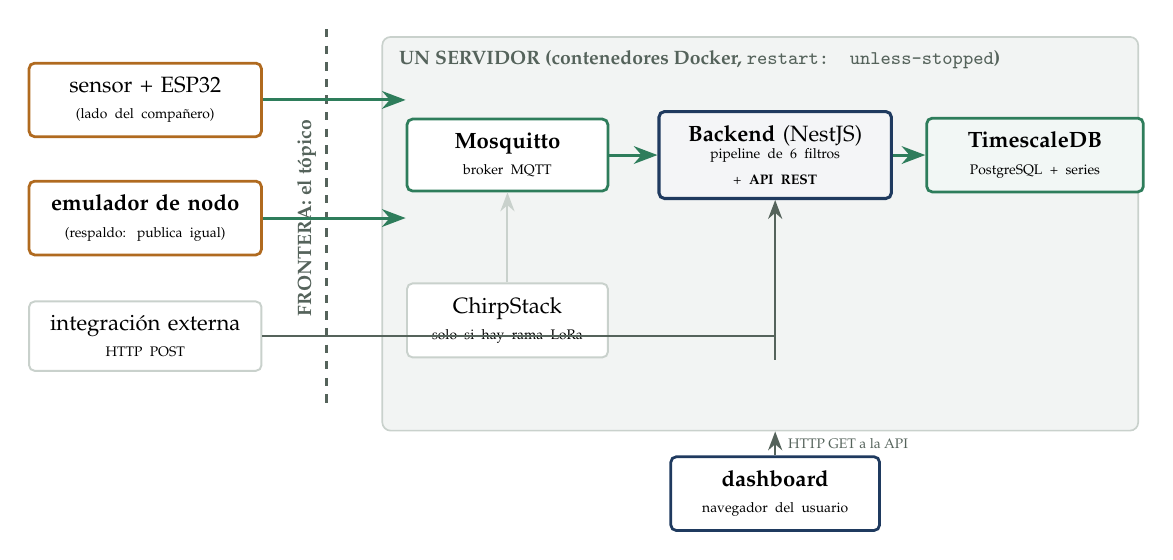
\begin{tikzpicture}[font=\scriptsize]

% lado emisores
\node[caja, text width=2.6cm, align=center, draw=ambar, line width=1pt] (n1) at (0,1.7)
  {sensor + ESP32\\ \tiny (lado del compañero)};
\node[caja, text width=2.6cm, align=center, draw=ambar, line width=1pt] (n2) at (0,0.2)
  {\textbf{emulador de nodo}\\ \tiny (respaldo: publica igual)};
\node[caja, text width=2.6cm, align=center, draw=grislinea] (n3) at (0,-1.3)
  {integración externa\\ \tiny HTTP POST};

% frontera
\draw[line width=1pt, color=gristexto, dashed] (2.3,2.6) -- (2.3,-2.2);
\node[etiqueta, font=\scriptsize\bfseries\color{gristexto}, rotate=90] at (2.05,0.2) {FRONTERA: el tópico};

% servidor
\node[grupo, minimum width=9.6cm, minimum height=5.0cm, anchor=west] (srv) at (3.0,0) {};
\node[font=\scriptsize\bfseries\color{gristexto}, anchor=north west] at (3.1,2.45)
  {UN SERVIDOR (contenedores Docker, \texttt{restart: unless-stopped})};

\node[caja, text width=2.2cm, align=center, draw=verdeacento, line width=1pt] (mq) at (4.6,1.0)
  {\textbf{Mosquitto}\\ \tiny broker MQTT};
\node[caja, text width=2.2cm, align=center, draw=grislinea] (cs) at (4.6,-1.1)
  {ChirpStack\\ \tiny solo si hay rama LoRa};
\node[caja, text width=2.6cm, align=center, draw=azuloscuro, line width=1.1pt, fill=azuloscuro!5] (be) at (8.0,1.0)
  {\textbf{Backend} (NestJS)\\ \tiny pipeline de 6 filtros\\ \tiny + \textbf{API REST}};
\node[caja, text width=2.4cm, align=center, draw=verdeacento, line width=1pt, fill=verdeacento!6] (db) at (11.3,1.0)
  {\textbf{TimescaleDB}\\ \tiny PostgreSQL + series};

\draw[flechagruesa] (n1.east) -- (mq.west|-n1.east);
\draw[flechagruesa] (n2.east) -- (mq.west|-n2.east);
\draw[flecha] (n3.east) -| (8.0,-1.6) -- (be.south);
\draw[flechagruesa] (mq.east) -- (be.west);
\draw[flecha, color=grislinea] (cs.north) -- (mq.south);
\draw[flechagruesa] (be.east) -- (db.west);

% dashboard afuera
\node[caja, text width=2.3cm, align=center, draw=azuloscuro, line width=1pt] (dash) at (8.0,-3.3)
  {\textbf{dashboard}\\ \tiny navegador del usuario};
\draw[flecha] (dash.north) -- node[nota, right=1pt, font=\tiny] {HTTP GET a la API} (be.south|-srv.south);

\end{tikzpicture}}
\caption{Despliegue: todos los componentes corren como contenedores en un único servidor. La
frontera con el trabajo del compañero es el tópico MQTT; el emulador de nodo publica en el mismo
tópico, de modo que la validación no depende del hardware.}
\label{fig:despliegue}
\end{figure}


\section{Evaluación de infraestructura}
\label{sec:infra}

\begin{table}[H]
\centering\footnotesize
\begin{tabular}{@{}L{2.4cm}L{2.4cm}L{7.6cm}@{}}
\toprule
\textbf{Componente} & \textbf{Selección} & \textbf{Razón determinante frente a alternativas} \\
\midrule
Broker MQTT & Mosquitto & C, $\sim$10\,MB de RAM, TLS y autenticación; EMQX/HiveMQ apuntan a millones de conexiones: desproporcionados \\
Persistencia & TimescaleDB & Un solo motor relacional y de series; InfluxDB obligaría a operar dos bases \\
Backend & TypeScript + NestJS & Tipos de la trama definidos una sola vez para backend y panel; módulos 1:1 con M1--M8; OpenAPI automático \\
Rama LoRa & ChirpStack & Autoalojable; publica en MQTT: converge a la vía principal \\
Despliegue & Contenedores Docker & Reproducible con un comando; reinicio automático; la Etapa 4 exige demostrar en condiciones realistas \\
\bottomrule
\end{tabular}
\caption{Decisiones de infraestructura. Las matrices completas están en el repositorio.}
\label{tab:infra}
\end{table}

\textbf{Restricciones:} RE-01 dedicación $\sim$15 h semanales; RE-02 proyecto individual coordinado
con el trabajo del compañero; RE-03 solo componentes abiertos; RE-05 umbral de aprobación del
70\,\%; RE-06 hardware no confirmado, mitigado con el emulador.

\chapter[Diseño del sistema]{Diseño del sistema}
\label{cap:diseno}

Este capítulo describe \emph{cómo} la plataforma cumple los requerimientos del capítulo anterior.
Siguiendo la recomendación de describir un sistema desde varias vistas \parencite{iso42010}, se presentan la estructura
estática (contenedores), los datos, la red y la seguridad, el comportamiento dinámico (secuencias),
el manejo del tiempo y el despliegue. Las notaciones son las reconocidas en la industria: el modelo
C4 \parencite{c4brown} para la vista de contenedores, diagramas entidad-relación \parencite{chen1976}
para los datos y diagramas de secuencia UML \parencite{uml251} para el comportamiento. Las figuras
se generan automáticamente desde la documentación versionada y, el modelo de datos, desde el esquema
real de la base, de modo que informe, documentación y base no pueden diferir; lo que aún no está
implementado se indica con su etapa.

\section{Vista de contenedores y frontera del trabajo}

La figura~\ref{fig:contenedores} muestra las piezas ejecutables y cómo se comunican; la frontera con
el trabajo del compañero —el tópico MQTT— ya se definió en la sección~\ref{sec:frontera}.

\begin{figure}[!htb]
\centering
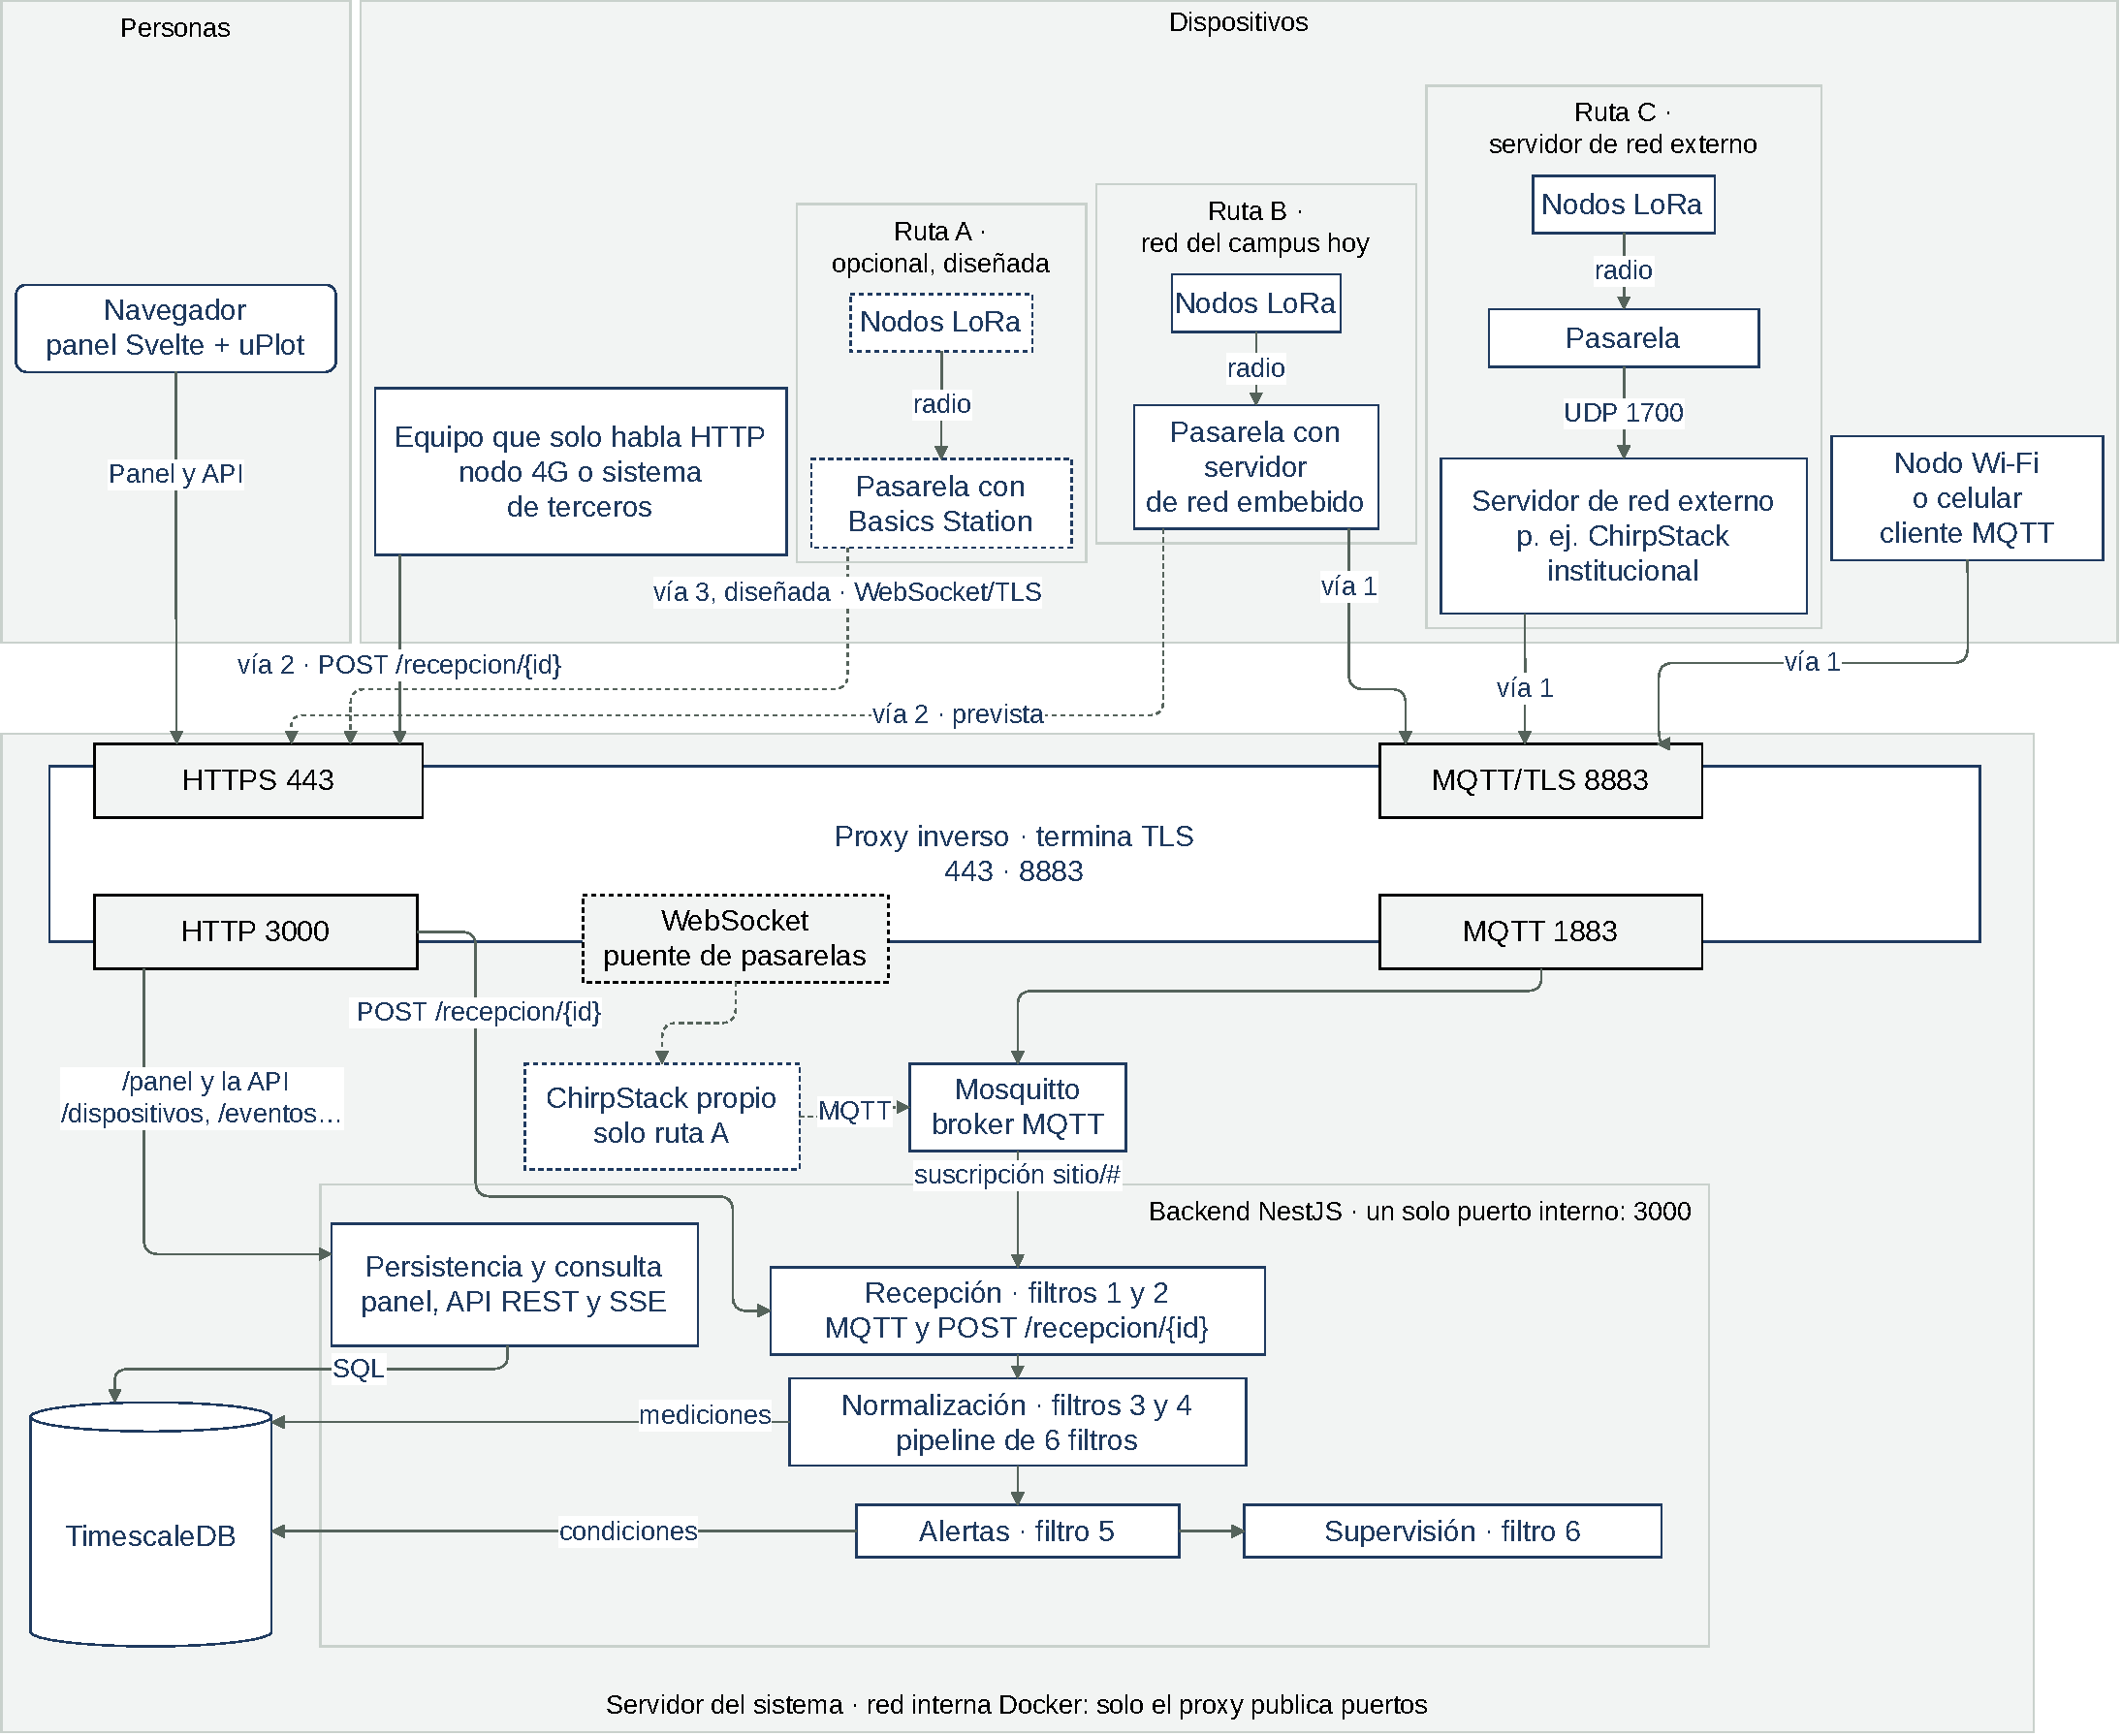
\includegraphics[width=\linewidth,height=0.62\textheight,keepaspectratio]{figuras/drawio/figura-4.1.pdf}
\caption{Vista de contenedores (modelo C4, nivel 2). La frontera del trabajo es el tópico MQTT: de un lado, la red de sensores del compañero (nodos y \emph{gateway}: en la ruta B la pasarela —la red del campus hoy— y en la ruta C un servidor de red externo publican al broker por TLS con su propia credencial (vía 1); en la ruta A, opcional, diseñada y punteada, la pasarela llega por WebSocket sobre TLS con \emph{Basics Station} a un ChirpStack propio (vía 3)); del otro, el proxy —único contenedor expuesto—, el broker y el backend. Un nodo Wi-Fi o celular publica directo por MQTT sobre TLS (vía 1); un equipo que solo habla HTTP entra por 443 con un token (vía 2) y cae en la misma tubería de seis filtros; el reporte HTTPS de la pasarela, variante prevista de la vía 2, va punteado. El navegador nunca se conecta al broker: consume la API del backend, que ya autenticó, validó y normalizó cada trama y, con la sesión de la Etapa 4, cada usuario verá solo los datos de su sitio (RF-41). Las cajas del backend llevan los filtros de la figura~\ref{fig:pipeline} que ejecutan y corresponden a los módulos M1, M2, M6, M4 y M5 del catálogo; M3, M7 y M8 son transversales o viven en el cliente.}
\label{fig:contenedores}
\end{figure}


Tres decisiones quedan visibles en la figura. Primero, hay \textbf{dos puntos de entrada siempre y tres a lo
sumo}: HTTPS para personas (443), MQTT sobre TLS para dispositivos y pasarelas de las rutas B y C (8883) y, solo
en la ruta A, opcional y punteada, UDP para los \emph{gateways} LoRaWAN (1700). Ese tercer puerto recibe un
protocolo sin autenticación ni cifrado propios (\emph{Semtech UDP Packet Forwarder}), así que la defensa
la dan el contenedor sin privilegios y el límite de tasa, no el protocolo. La base de datos y la
consola de administración de ChirpStack nunca se exponen. Segundo, \textbf{el navegador nunca se conecta al
broker}: consume la API del backend, que ya autenticó, validó y normalizó cada trama. La alternativa
—suscribir el navegador al broker por WebSocket— habría expuesto el broker a Internet y puesto
credenciales MQTT en el código del cliente. Tercero, \textbf{el servidor de red LoRaWAN es un productor más} hacia el
broker: una trama LoRaWAN decodificada y una trama Wi-Fi directa son indistinguibles para la
plataforma después del filtro de análisis, que es lo que resuelve la causa C2 (hardware atado a la
plataforma).

Los ocho módulos del análisis (capítulo~\ref{cap:especificacion}) se reparten así: M1 recepción y M2
normalización forman el servicio de recepción del backend, es decir, el pipeline; M4 supervisión de
salud es el barrido periódico; M5 persistencia y consulta es la API sobre TimescaleDB; M6 alertas es el
servicio de umbrales. No aparecen como cajas M3 inventario y aprovisionamiento ni M7 seguridad e
identidad, transversales al backend y previstos para la siguiente etapa, ni M8 interfaz, que es el
panel y corre en el navegador.

\section{Modelo de datos}

El modelo (figura~\ref{fig:modelo-datos}) tiene 18 entidades y una idea rectora: \textbf{el modelo
interno es único}. No importa por qué vía ni en qué formato llegó una trama; una vez superado el
pipeline, todo se guarda con la misma forma. Esa uniformidad es la respuesta a la causa C1 (formatos
dispares). El esquema está en tercera forma normal, y no más allá porque la cuarta y la quinta resuelven dependencias multivaluadas y de reunión que este modelo no tiene: cada hecho vive en una sola tabla y las
relaciones muchos a muchos se resuelven con entidades de asociación (\texttt{canal} es dispositivo por
magnitud; \texttt{usuario\_sitio}, usuario por sitio). Las únicas redundancias son deliberadas y se
llaman «foto por valor»: la unidad copiada en cada medición y el umbral vigente copiado en cada evento,
para que cambiar un catálogo no reinterprete el pasado.

\begin{figure}[!tbp]
\centering
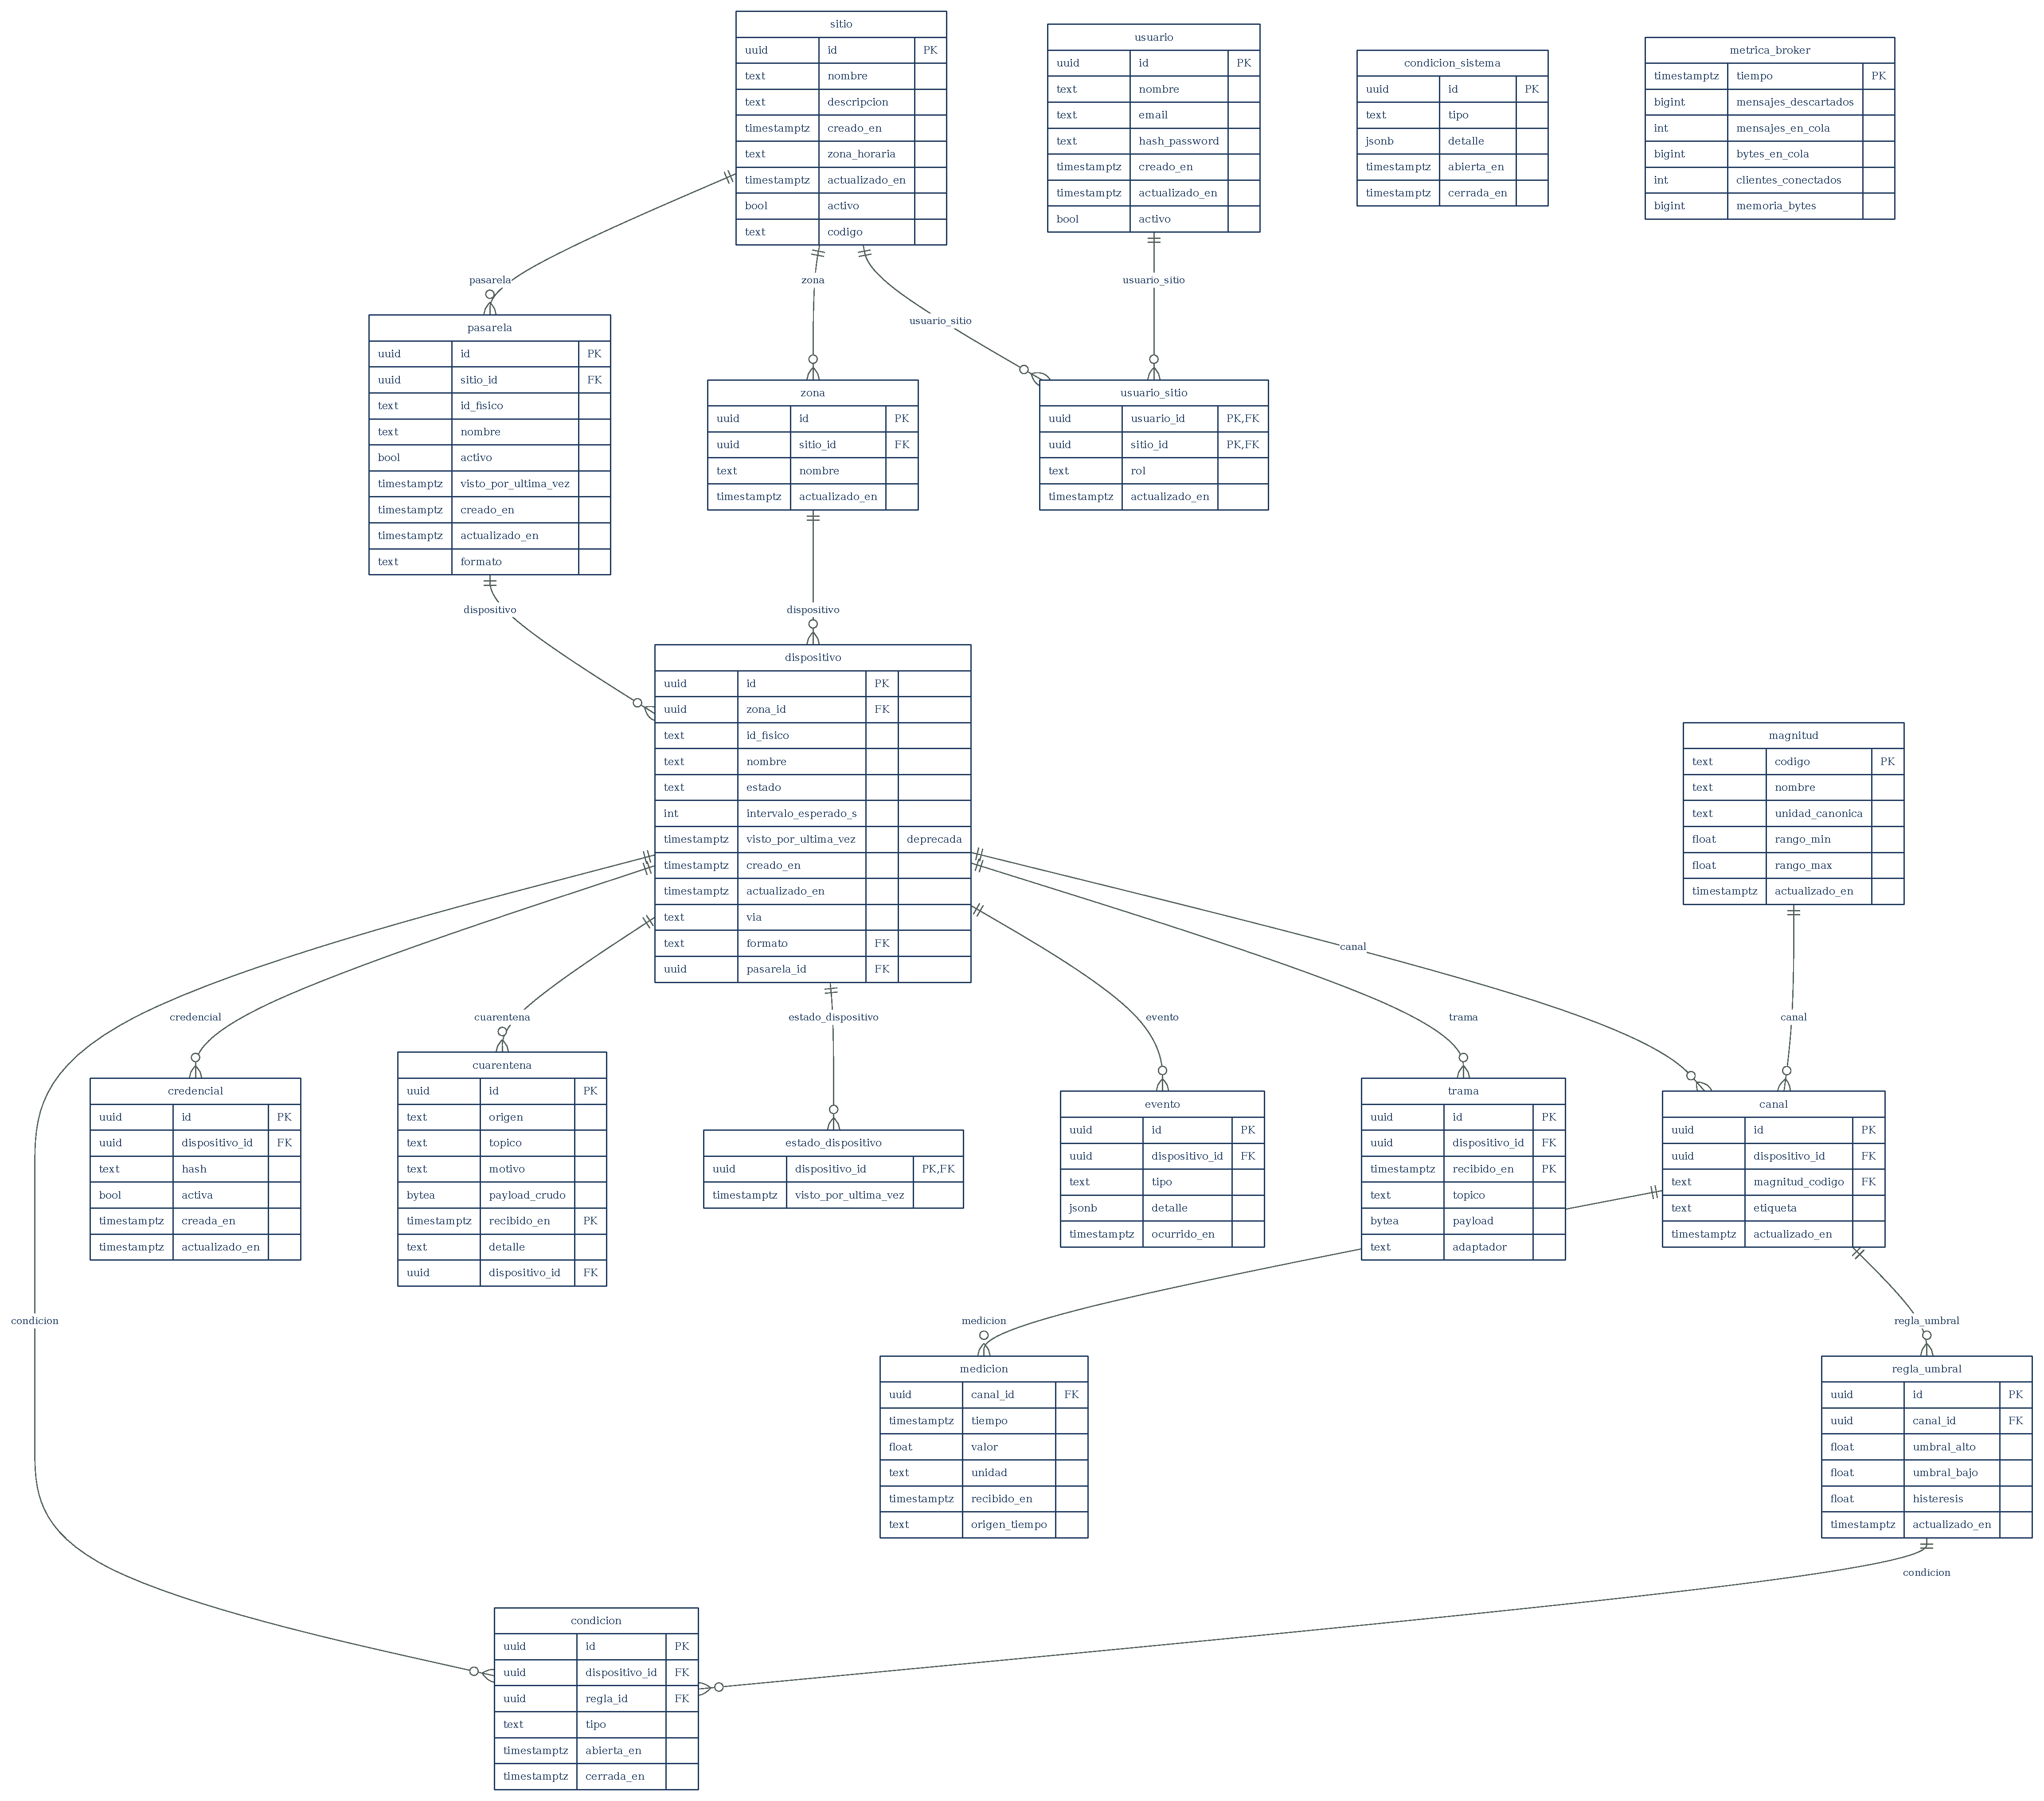
\includegraphics[width=\linewidth,height=0.74\textheight,keepaspectratio]{figuras/render/modelo-datos.pdf}
\caption[Modelo de datos, generado desde el esquema real]{Modelo de datos (diagrama entidad-relación, notación \emph{crow's foot}), generado desde el esquema real de la base de datos. 22 entidades: la organización (\texttt{sitio}, \texttt{zona}, \texttt{usuario} y \texttt{usuario\_sitio}), el acceso de las personas (\texttt{sesion} y \texttt{acceso}), lo propio de cada una (\texttt{preferencia} y \texttt{mensaje\_soporte}), el inventario (\texttt{dispositivo}, \texttt{pasarela}, \texttt{canal}, \texttt{credencial}, \texttt{estado\_dispositivo} y el catálogo \texttt{magnitud}), las series de tiempo (\texttt{medicion}), el estado (\texttt{regla\_umbral}, \texttt{condicion}, \texttt{evento}), lo crudo ---\texttt{trama}, aceptada, y \texttt{cuarentena}, rechazada y atribuida al dispositivo cuando se sabe cuál es--- y la salud del propio sistema (\texttt{condicion\_sistema}, \texttt{metrica\_broker}). \texttt{medicion}, \texttt{trama}, \texttt{cuarentena}, \texttt{metrica\_broker} y \texttt{acceso} son hypertables particionadas por tiempo. Una medición pertenece a un \emph{canal} —dispositivo más magnitud— y no al dispositivo: un nodo que mide temperatura y humedad produce dos series.}
\label{fig:modelo-datos}
\end{figure}



Las decisiones del modelo y su justificación —por qué la medición cuelga del canal, por qué la credencial es una entidad aparte, por qué la cuarentena vive aparte de las series— se detallan en el cuadro~\ref{tab:decisiones-datos} (anexo~\ref{anx:evaluacion}). Lo que el diagrama no muestra por convención también está diseñado: el esquema sigue un conjunto de \textbf{convenciones de calidad} verificadas contra la base real —toda restricción con nombre explícito y prefijo (\texttt{pk\_}, \texttt{fk\_}, \texttt{uq\_}, \texttt{ck\_}), un índice por cada clave foránea (PostgreSQL no lo crea solo y sin él cada unión recorre la tabla completa), auditoría con \texttt{actualizado\_en} mantenida por disparador en toda tabla mutable, baja lógica en lugar de borrado, dominios cerrados como \texttt{CHECK} y catálogos donde el usuario administra los valores, y comentarios \texttt{COMMENT ON} en las columnas cuya razón de ser no es obvia, de modo que la documentación viaja con la base—. El esquema evoluciona por \textbf{migraciones numeradas} (\texttt{01-esquema}, \texttt{02} unicidad
de condición por regla, \texttt{03} zona horaria por sitio, \texttt{04} serialización uniforme de
instantes, \texttt{05} convenciones de calidad, \texttt{06} clave natural única de la serie, \texttt{07} dominio cerrado de \texttt{cuarentena.motivo}): nunca se edita un archivo ya aplicado. Una instalación nueva ejecuta todas en orden; una
base existente aplica solo las nuevas.

\section{Topología de red y seguridad en capas}

La figura~\ref{fig:red} (anexo~\ref{anx:figuras}) muestra los tres segmentos de red y qué cruza cada frontera. Los dispositivos
del sitio abren únicamente \textbf{conexiones salientes}, de modo que el router del cliente no necesita
puertos abiertos ni configuración alguna (RNF-10): una organización sin personal técnico (causa C4)
conecta un sensor sin tocar su red.


La seguridad se diseñó en capas, asumiendo en cada una que la anterior falló: (1)~red: solo 443, 8883
y 1700/udp publicados; (2)~TLS obligatorio en producción; (3)~identidad: broker sin conexiones anónimas,
usuario MQTT igual al identificador físico, contraseñas con hash; (4)~lista de control de acceso (ACL) por
patrón: cada dispositivo escribe solo bajo su propio identificador, lo que impide la suplantación entre
nodos; (5)~el pipeline valida y envía a cuarentena; (6)~datos: base sin puerto expuesto, una credencial
por servicio; (7)~contenedores sin escalada de privilegios, con versión de imagen fijada y techo de
recursos; (8)~operación: respaldos, secretos fuera del repositorio. Las capas 1, 3, 4, 5 y 7 están
implementadas y \textbf{verificadas} en el despliegue de desarrollo: una publicación anónima o con clave
incorrecta es rechazada, y un dispositivo que intenta publicar en el tópico de otro es descartado sin
que el suscriptor llegue a recibir el mensaje.

\section{Comportamiento}

\subsection{Aprovisionamiento de un dispositivo}

La figura~\ref{fig:sec-alta} (anexo~\ref{anx:figuras}) describe cómo un dispositivo pasa de desconocido a reconocido. Es el flujo que ataca la causa C4: una persona sin perfil técnico registra un dispositivo, hoy por la API y desde el panel en la Etapa~4; según la vía declarada, el sistema genera la credencial, la muestra \textbf{una vez}, guarda su hash y registra
al dispositivo en el broker con una lista de acceso restringida a su propio tópico. El estado «en línea»
no nace del alta, sino del \textbf{primer mensaje autenticado}.


\subsection{Recepción de una trama: el pipeline}

La figura~\ref{fig:sec-pipeline} (anexo~\ref{anx:figuras}, apaisada para que se lea) detalla el aporte central del trabajo, organizado según el patrón
\emph{pipes and filters} \parencite{posa1}. Cada filtro tiene una salida que
continúa y una de rechazo hacia la cuarentena; ninguna lectura llega a las series sin superar los cuatro
primeros, y los dos últimos no escriben series sino condiciones.
El orden importa: autenticar primero evita gastar recursos en tramas de desconocidos; validar antes de
guardar evita que una lectura imposible llegue a la serie. Los dos últimos filtros trabajan a distinta escala: el de alertas
evalúa \emph{cada lectura} guardada, porque un umbral se cruza por valor; el de supervisión se ejecuta
\emph{una vez al cerrar la trama}, porque lo que registra no es un dato sino un hecho del enlace —este
dispositivo se comunicó—, y por eso marca al dispositivo como visto aunque sus lecturas hayan ido a
cuarentena: un nodo que publica tramas malformadas está vivo y mal configurado, no en silencio, y
confundir ambos casos manda al operador a buscar la falla donde no está. El filtro de análisis delega en \textbf{adaptadores} intercambiables —SenML
\parencite{rfc8428} como contrato nativo y un formato plano para nodos simples—, de modo que admitir el formato de un nuevo
fabricante es agregar una clase, no modificar el pipeline (RF-04). La entrega desde el broker es
«al menos una vez»: QoS~1 con sesión persistente, de modo que si el backend cae el broker conserva la
cola, hasta un tope de mensajes, y la entrega al volver. Eso admite reentregas, y por ello la inserción en la serie es idempotente
sobre la clave natural canal e instante: una lectura repetida se ignora sin volver a evaluar umbrales
(RF-06, RF-10). No se usa QoS~2: su garantía vale por salto cliente–broker \parencite{mqttoasis}, no
hasta la base; el receptor debe ser idempotente igual y, con eso, QoS~1 basta.


Un detalle de diseño que no se ve en la secuencia: el pipeline solo corre \emph{cuando llega} una trama,
así que no puede notar que un dispositivo \emph{dejó} de transmitir. Por eso existe un \textbf{supervisor
periódico} (M4) que compara la última recepción de cada dispositivo con su intervalo esperado y abre la
condición «sin comunicación» cuando el silencio supera dos intervalos. Un mensaje perdido no es una
caída; dos seguidos, sí. Las alertas por umbral (M6) usan \textbf{histéresis}: la condición abre al cruzar
el umbral y cierra solo al volver un margen más adentro, para que un valor que oscila alrededor del
límite no dispare y cierre alertas sin parar.

\subsection{Panel en tiempo real}

La figura~\ref{fig:sec-tiemporeal} (anexo~\ref{anx:figuras}) muestra los dos tiempos del panel. El histórico llega
\textbf{agregado por la base de datos} con \texttt{time\_bucket}: cientos de puntos, no millones. Las lecturas
nuevas las empuja el backend por un canal SSE, cifrado tras el proxy, que solo anuncia
lo ya guardado, rechaza otro origen u otro host y limita los flujos abiertos; desde la Etapa~4 se abre con la sesión del
panel, como recomienda OWASP para WebSocket \parencite{owaspws}. El navegador nunca toca el broker. Toda consulta valida sus entradas (identificadores, fechas, un intervalo de una lista
cerrada) y usa parámetros, nunca texto interpolado. El \textbf{contrato de la API se
genera desde el código}, en OpenAPI 3.0 \parencite{openapi303}, desde los controladores, así no puede describir rutas
inexistentes; se sirve junto a la API y se versiona como el acuerdo que consumirá el panel.


\section{Despliegue y presupuesto de recursos}

La figura~\ref{fig:despliegue} (anexo~\ref{anx:figuras}) muestra el despliegue: un servidor, una red interna y
cuatro contenedores —proxy, broker, backend y base de datos—, más ChirpStack solo en la ruta A, con una
base propia dentro del mismo PostgreSQL. El backend no guarda estado, por lo que puede recrearse sin pérdida. Cada contenedor tiene versión de imagen
fijada, no puede escalar privilegios, se reinicia solo ante fallas y tiene un techo de memoria y CPU.


La suma de techos es de 1,6~GB en la ruta B —los cuatro contenedores ya implementados— y de
1,95~GB con ChirpStack (ruta A), ambas dentro del RNF-17 (consumo de a lo más 2~GB de RAM); el consumo real se
mide en la Etapa~4. Los
límites cumplen además una segunda función: definen el \textbf{entorno de referencia} del banco de pruebas
de la Etapa~4, para que la comparación no dependa del equipo de desarrollo.

\textbf{Alojamiento.} La recomendación es un \textbf{servidor privado virtual (VPS) internacional de 2~vCPU y 4~GB},
del orden de CLP~6\,000 mensuales, para la validación y un primer sitio, con un VPS nacional como alternativa si se
exigen datos en Chile. La comparación de cinco alternativas con precios fechados y el costo por retención están en el
anexo~\ref{anx:evaluacion} (cuadro~\ref{tab:alojamiento}).

\textbf{Tiempo.} Todo instante se guarda en UTC y cada sitio declara su zona por nombre (\texttt{America/Santiago}):
como Chile cambia de hora por decreto, toda pregunta de «día» se responde dentro de la base, en la zona del sitio
(reglas y verificación en el anexo~\ref{anx:evaluacion}, sección~\ref{sec:tiempo}).

\textbf{Trazabilidad.} Cada elemento de diseño materializa requerimientos del catálogo
(cuadro~\ref{tab:trazabilidad-diseno}, anexo~\ref{anx:evaluacion}); RF-29 queda pendiente: el backend aún no
publica \emph{Last Will}.

\chapter{Implementación y pruebas iniciales}
\label{cap:pruebas}

\section{Qué está implementado}

El cuadro~\ref{tab:implementado} resume cada módulo; en horas, el núcleo mínimo (OE4) está hecho en un 78\,\% (sección~\ref{sec:seguimiento}).

\begin{table}[tb]
\centering\footnotesize
\begin{tablaseg}
\begin{tabular}{@{}L{2.5cm}L{6.7cm}L{3.8cm}@{}}
\toprule
\textbf{Módulo} & \textbf{Implementado y probado} & \textbf{Falta} \\
\midrule
M1 Recepción & MQTT con TLS y HTTP, credencial propia; LoRaWAN por pasarela (ruta B, en terreno) y ChirpStack (ruta C) & Ruta C en terreno \\
M2 Normalización & Seis filtros con cuarentena; formato del alta; tope por emisor & Pruebas del contrato \\
M3 Registro & Alta, baja y rotación por API, todo o nada; pasarelas & Pantalla (Etapa~4) \\
M4 Supervisión & Silencio según el intervalo esperado de cada uno & Batería; enlace; \emph{Last Will} \\
M5 Series & TimescaleDB, 22 migraciones, API, CSV y JSON, canal en vivo & XLSX; rango a medida \\
M6 Alertas & Umbral con histéresis; alarma de la cola del broker & Notificación \\
M7 Seguridad & Claves con hash, ACL por rol, mínimo privilegio, sin \texttt{NET\_RAW}; sesión y roles por sitio & Pantalla de sesión; auditoría \\
M8 Panel & Semáforo; inventario filtrable; ficha; canal callado & Salud del sitio \\
\bottomrule
\end{tabular}
\end{tablaseg}
\caption[Estado de la implementación por módulo]{Estado de la implementación por módulo al 28 de octubre de 2026.}
\label{tab:implementado}
\end{table}

\section{Método de prueba}

Se prueba en tres niveles, todos repetibles con un comando (anexo~\ref{anx:pruebas}). Las 445 pruebas unitarias del backend y las 165 del panel corren sin base ni broker, con tipos estrictos y análisis estático. \textbf{Banco
desechable}: una segunda pila con base, broker con su plugin de seguridad, backend y proxy reales, datos en memoria y un
emulador de nodos que imita relojes rotos, pérdidas y deriva; sobre él corren casos fijos de carga, carreras,
caídas, TLS, alta por API, LoRaWAN y cola del broker. \textbf{Verificador de concordancia}: 49 pasos que comparan informe, documentación, base y API. Cada comprobación nueva se ejecuta primero contra el error \emph{plantado}: una prueba vale solo si falla ante la falla.

\section{Resultados frente a los requerimientos}

El cuadro~\ref{tab:resultados} reúne los resultados preliminares.

\begin{table}[tb]
\centering\footnotesize
\begin{tablaseg}
\begin{tabular}{@{}L{2.1cm}L{4.1cm}L{5.2cm}L{1.6cm}@{}}
\toprule
\textbf{Requisito} & \textbf{Prueba} & \textbf{Resultado} & \textbf{Estado} \\
\midrule
RNF-01 y 02 & 120 nodos emulados, 90~s & 59,7 tramas/s, 0 perdidas; p95 de 3~ms & Cumple \\
Capacidad & Picos de 400 y 800 nodos & Sin pérdida hasta 409 tramas/s & Medida \\
RNF-03 & Caídas emuladas & Todas; 3 alarmas falsas (eran 108) & Cumple \\
RNF-05 y 06 & Backend caído 20~s; base, 15~s & 0 perdidas; reconexión sola & Parcial \\
RF-10 & La misma lectura ×20 a la vez & Una fila por canal y una trama cruda & Cumple \\
RF-12 & Cinco sobre el umbral a la vez & Una condición, sin errores & Cumple \\
RF-05 y RF-07 & Malformadas, sin alta, otro sitio & Cuarentena con motivo; ninguna señal de vida falsa & Cumple \\
RF-40, RF-42 & Credencial ajena; sin CA; sin TLS & Rechazadas; claves con hash (RNF-08) & Cumple \\
RF-02 & JSON oficial de los fabricantes; pasarela del campus & 46 de 46 del banco LoRaWAN; pasarela real en terreno & Cumple \\
RNF-17 & Carga sostenida y pico & 174~MiB (sin proxy) y 324~MiB (pico, con proxy); al iniciar sesión, el backend llega a 321~MiB (docs/16 §59) & Preliminar \\
\bottomrule
\end{tabular}
\end{tablaseg}
\caption[Resultados preliminares frente a los requerimientos]{Resultados preliminares. «Parcial»: falta el broker de producción (RNF-05); RNF-02, medido sin red real, se repite en el servidor.}
\label{tab:resultados}
\end{table}

\textbf{Mejoras derivadas de las pruebas.} Las pruebas cambiaron el diseño, no solo lo confirmaron. Las 108 alarmas falsas de silencio bajaron a 3 al declarar el intervalo esperado como el silencio normal (dos periodos), sin tocar RNF-03. Bajo duplicados simultáneos se duplicaba la trama cruda y una condición abortaba el pipeline: ahora se procesa un mensaje a la vez y se confirma al broker después de guardar. El broker descartaba sin aviso: hoy tiene topes de cola y una alarma sobre su contador. Dar de baja un dispositivo frenaba hasta 5~s la recepción de todos; hoy, 20~ms. En terreno, el reloj de la pasarela venía cuatro días atrasado: una tolerancia de diez minutos y la condición «reloj desviado» separan ese caso de una lectura inválida. La corrida de 24~h cambió el firmware (omite el sensor que no responde; vigilante de 120~s) y el panel (marca el «canal callado» cuando una magnitud deja de llegar).

\section{Validación preliminar y limitaciones}

El sistema funciona de extremo a extremo con nodos emulados; con el nodo propio, un ESP32 con sensores de aire, suelo y temperatura (CLP~26\,530 en piezas más la placa; figura~\ref{fig:cableado}), 24~h por Wi-Fi con TLS: 1\,440 de 1\,440 tramas, sin reinicios; y con la red LoRaWAN del campus: el 20 de octubre la pasarela real publicó por TLS con su credencial y dos nodos entraron de punta a punta, 813 mediciones en 3~h. La misma serie de 180 lecturas entró completa por las tres entradas (MQTT, HTTP y pasarela): 0 pérdidas, 0 duplicados y p95 de 4 a 157~ms; por HTTP, el tope de una trama por segundo por dispositivo obliga a agrupar lecturas. Desde el 3 de noviembre la pila corre además en un servidor de prueba de la institución (anexo~\ref{anx:despliegue}). Faltan la validación de RNF-17 y RNF-18 en un servidor de recursos modestos (OE5, Etapa~4) y la ruta C en terreno.

\chapter[Metodología y planificación]{Metodología y planificación}
\label{cap:metodologia}

\section{Marco metodológico}

Se adopta \textbf{PPDIOO} (Cisco) como ciclo de vida de ingeniería, por tres razones: es el marco propio
del dominio de redes, corresponde a la especialidad del profesor guía, y sus fases coinciden con las
cuatro etapas de evaluación (Prepare/Plan $\rightarrow$ Etapa 1; Design $\rightarrow$ Etapa 2; Implement
$\rightarrow$ Etapa 3; Operate/Optimize $\rightarrow$ Etapa 4).

Se descarta Scrum como marco de gestión de equipo —el proyecto es unipersonal y sus ceremonias carecen
de sentido— pero \textbf{se conservan sus artefactos de planificación}: el backlog con épicas, historias
de usuario, criterios de aceptación y estimaciones. No es solo preferencia metodológica: la pauta asigna
el 20\,\% de esta etapa al backlog y mide el avance de las siguientes como porcentaje de tareas
completadas. PPDIOO define qué fases hay; el backlog, cómo se mide el avance.

Los estándares de referencia siguen al SWEBOK v4 \parencite{swebok} en sus áreas de requerimientos
(cap.~1), arquitectura y diseño (caps.~2--3), pruebas (cap.~5) y gestión de configuración (cap.~7): todo
el trabajo se versiona en un repositorio git con mensajes descriptivos, y la retroalimentación del
profesor guía se registra en bitácora con trazabilidad indicación $\rightarrow$ cambio $\rightarrow$
evidencia.

\section{Calendario oficial}

\begin{table}[H]
\centering\small
\begin{tabular}{@{}L{6.6cm}C{2.8cm}C{3.0cm}@{}}
\toprule
\textbf{Etapa} & \textbf{Sprint} & \textbf{Entrega} \\
\midrule
1 --- Problema, objetivos, requerimientos & 17 ago -- 4 sep & \textbf{4 de septiembre} \\
2 --- Diseño e implementación inicial & 7 sep -- 2 oct & 2 de octubre \\
3 --- Mejoras, pruebas, validación preliminar & 5 -- 30 oct & 30 de octubre \\
4 --- Validación final e informe & 2 nov -- 4 dic & 4 de diciembre \\
\bottomrule
\end{tabular}
\caption{Calendario oficial (pauta del 17 de agosto de 2026). Presupuesto a $\sim$15 h semanales:
$\sim$240 horas.}
\label{tab:calendario}
\end{table}

\section{Backlog y verificación de viabilidad}

El backlog contiene \textbf{65 elementos} —25 historias de usuario y 40 tareas técnicas, agrupados en 14 épicas—
estimados en horas ideales, ajustados tras el pivote del 2 de septiembre: los elementos ligados al
protocolo descartado se reformularon hacia el contrato SenML y el pipeline, con un efecto neto de
$-10$ horas en el núcleo demostrativo ($\sim$155 h). El backlog completo está en el
anexo~\ref{anx:backlog}.

\begin{quote}
\textbf{Criterio de demostración:} el prototipo demuestra la tesis si recibe tramas por al menos dos
vías (MQTT y HTTP), las normaliza al modelo interno, detecta que un dispositivo dejó de reportar, lo
presenta en el panel con el estado de cada dispositivo, y permite exportar los datos en formato
abierto.
\end{quote}

La verificación numérica —sumando programáticamente las estimaciones— arrojó el hallazgo de mayor
consecuencia práctica de la etapa: \textbf{el backlog completo ($\sim$272 h) excede el presupuesto y no es
ejecutable íntegro; el núcleo demostrativo ($\sim$155 h) cabe con holgura} ($\sim$+35\,\% con el
calendario oficial). En consecuencia, \textbf{el compromiso del proyecto es el núcleo} y los 32 elementos restantes
son alcance condicional, ejecutable solo contra holgura verificada al cierre de cada etapa. El
fundamento: la pauta mide el avance como porcentaje de tareas completadas, de modo que comprometer el backlog íntegro y ejecutar solo el núcleo arrojaría cerca de un 60\,\% —bajo el umbral—, mientras que comprometer el núcleo y ejecutarlo arroja el 100\,\%.

La distribución temporal también se corrigió: la asignación inicial concentraba la implementación en la
Etapa 3 (162\,\% de su capacidad) cuando la pauta solo exige allí el 50\,\%; se trasladaron $\sim$37
horas del núcleo a la Etapa 4, verificando que el umbral del 50\,\% se cumple (53\,\%).

\section{Seguimiento del backlog en la Etapa 2}
\label{sec:seguimiento}

La pauta evalúa el avance como el cumplimiento de las tareas de diseño previstas en el backlog. El
cuadro~\ref{tab:seguimiento} compara lo planificado con lo ejecutado al cierre de la etapa; el detalle
con evidencia por ítem se mantiene en la documentación del repositorio.

\begin{table}[H]
\centering\scriptsize
\setlength{\tabcolsep}{4pt}
\begin{tablaseg}
\begin{tabular}{L{1.2cm}L{5.4cm}C{0.6cm}L{6.2cm}}
\filaencab \encab{Ítem} & \encab{Tarea} & \encab{h} & \encab{Estado al cierre} \\
TT-01 & Componer el entorno con contenedores: TimescaleDB, Mosquitto y ChirpStack orquestados, con un único comando de arranque & 6 & Hecho: docker-compose con TimescaleDB y Mosquitto; ChirpStack diseñado, pendiente de gateway \\
TT-02 & Inicializar el proyecto TypeScript + NestJS con estructura de módulos correspondiente a M1–M8 & 4 & Hecho: backend NestJS con módulos M1, M2, M4, M5, M6 \\
TT-03 & Configurar verificación automática: tipos, formato y ejecución de pruebas & 3 & Parcial: pruebas de solo lectura y guardianes; faltan ESLint y pruebas unitarias \\
TT-04 & Documentar el procedimiento de puesta en marcha en el repositorio & 1 & Hecho: READMEs de plataforma y backend \\
TT-05 & Diagrama de arquitectura de componentes, con los ocho módulos y sus dependencias & 5 & Hecho: vista de contenedores C4 (fig. 4.1) \\
TT-06 & Diagrama de topología de red con segmentación de dispositivos IoT (RNF-09) y sentido de las conexiones (RNF-10) & 6 & Hecho: topología de red (fig. 4.3) \\
TT-07 & Modelo de datos entidad-relación con al menos ocho entidades & 6 & Hecho: ER de 13 entidades generado desde la base (fig. 4.2) \\
TT-08 & Diagrama de flujo de recepción, desde la recepción hasta la persistencia, para los tres transportes & 4 & Hecho: secuencia del pipeline (fig. 4.5) \\
TT-09 & Diagrama de secuencia del aprovisionamiento de un dispositivo nuevo & 3 & Hecho: secuencia de aprovisionamiento (fig. 4.4) \\
TT-10 & Registro de decisiones de diseño con su justificación & 2 & Hecho: tablas de decisiones en el cap. 4 y bitácora \\
TT-11 & Esquema del modelo interno y contrato del tópico MQTT (nombres, unidades, identidad) & 3 & Hecho: docs/08, docs/10 §1; tópico sitio/·/dispositivo/·/magnitud \\
TT-12 & Catálogo de tipos de sensor y unidades aceptadas, con umbrales de disparo y restauración & 6 & Parcial: 5 magnitudes con rango; ampliar con los sensores reales \\
TT-13 & Especificación del contrato de la API en OpenAPI, generada desde el código & 3 & Pendiente el contrato OpenAPI; la API existe (cinco endpoints) \\
TT-14 & Política de QoS, reintento y cuarentena & 2 & Hecho: QoS 1, reconexión, cuarentena con motivo \\
TT-15 & Procedimiento de asignación de identidad y gestión de claves AES por sitio & 2 & Parcial: gestión de credenciales documentada (docs/11 §7); claves LoRaWAN dependen de ChirpStack \\
HU-01 & Publicar una trama SenML por MQTT o HTTP desde un sensor sin infraestructura intermedia & 6 & Parcial: MQTT sí; HTTP en la Etapa 3 \\
TT-16 & Validador de esquema SenML y analizador de tramas & 3 & Hecho: adaptador SenML \\
TT-19 & Esquema de base de datos y migraciones versionadas & 5 & Hecho: esquema + 4 migraciones \\
TT-24 & Comparar al menos tres alternativas de alojamiento con criterios ponderados & 4 & Pendiente \\
TT-25 & Cuantificar el costo mensual y anual de operación en CLP y USD & 3 & Pendiente \\
TT-26 & Redactar la recomendación de despliegue justificada & 1 & Parcial: vista de despliegue y presupuesto de recursos; falta el costo por alternativa \\
TT-35 & Documento de diseño de la Etapa 2, con todos los diagramas & 6 & Parcial: borrador completo del informe (31 págs.); falta pulir e incorporar retroalimentación \\
HU-03 & Publicar eventos en MQTT desde dispositivos que ya usan ese transporte & 4 & \textbf{Adelantado} (plan.\ E3), hecho: publicado y probado con mosquitto\_pub \\
HU-04 & Adaptador para un formato no SenML (extensibilidad de la recepción) & 7 & \textbf{Adelantado} (plan.\ E4), parcial: adaptador plano; se cierra con la trama real \\
TT-17 & Pipeline de normalización al modelo interno (seis filtros) con cuarentena & 6 & \textbf{Adelantado} (plan.\ E3), hecho: seis filtros verificados \\
HU-06 & Configurar umbrales por dispositivo para generar un evento al cruzarlos & 4 & \textbf{Adelantado} (plan.\ E3), parcial: motor listo; falta interfaz \\
TT-18 & Normalización de marcas temporales, tolerando nodos sin reloj confiable & 2 & \textbf{Adelantado} (plan.\ E3), hecho: tiempoPlausible \\
TT-20 & Autenticación de la recepción mediante credencial por sitio & 4 & \textbf{Adelantado} (plan.\ E3), hecho: credencial por dispositivo + ACL \\
\end{tabular}
\end{tablaseg}
\caption{Backlog de la Etapa 2 (22 ítems, 84~h) frente a lo ejecutado, más los ítems adelantados de etapas posteriores.}
\label{tab:seguimiento}
\end{table}

De los 22 ítems planificados para la etapa, 13 están completos, 6 parciales con su faltante identificado y 3 pendientes (alojamiento, costos y el contrato OpenAPI). Seis ítems de las Etapas~3 y~4 se adelantaron; ese margen se invirtió en el capítulo de diseño y en el método de generación y verificación de figuras.

\section{Riesgos}

\begin{table}[H]
\centering\small
\begin{tabular}{@{}lL{3.8cm}L{2.2cm}L{5.0cm}@{}}
\toprule
 & \textbf{Riesgo} & \textbf{Estado} & \textbf{Mitigación} \\
\midrule
R1 & Hardware de sensores no disponible & Activo & Emulador de nodo por software; el sensor físico demuestra el caso, el emulador la carga \\
R2 & Sin acceso a partes interesadas & Activo & Escalar vía profesor guía; documentar el intento; fuentes secundarias \\
R3 & Ambigüedad de fechas & \textbf{Cerrado} & Calendario oficial publicado el 24/08 \\
R4 & Alcance excesivo & \textbf{Confirmado y controlado} & Núcleo comprometido vs.\ alcance condicional; revisión de holgura por etapa \\
R5 & Protocolo inadecuado al patrón de uso & \textbf{Cerrado} & Se materializó y resolvió: Contact ID descartado el 02/09; el transporte es MQTT y el formato SenML (sección~\ref{sec:transporte}) \\
\bottomrule
\end{tabular}
\caption{Registro de riesgos.}
\label{tab:riesgos}
\end{table}

\chapter{Conclusiones de la etapa}

\textbf{Sobre la implementación.} Más de la mitad del núcleo está hecha, medida en horas, y funciona de extremo a
extremo: registro por API con credencial propia, recepción por MQTT con TLS y por las dos rutas LoRaWAN, pipeline de
seis filtros con cuarentena, supervisión del silencio, alertas por umbral, consulta, exportación y panel en vivo
(capítulo~\ref{cap:pruebas}).

\textbf{Sobre las pruebas.} Los requisitos medibles de esta etapa se cumplen en el banco: 59,7 tramas por segundo sin
pérdida frente a las 50 exigidas, un p95 de 3~ms frente a 2~s, toda caída detectada con 3 alarmas falsas y ninguna
lectura perdida ante caídas del backend y de la base. Además, las pruebas corrigieron el diseño en cinco puntos.

\textbf{Sobre la concordancia y el consumo.} Figuras y modelo de datos se generan desde la documentación y el esquema
real; un verificador de más de 150 comprobaciones falla si informe, documentación o sistema difieren, y cada
comprobación nueva se prueba antes contra el error plantado. Bajo carga, lo construido consume 174~MiB; RNF-17 (2~GB)
se valida en la Etapa~4.

\textbf{Sobre la retroalimentación y lo que sigue.} Las observaciones de la Etapa~1 y del 29 de septiembre están
incorporadas y la entrevista del 5 de octubre adelantó la exportación (sección~\ref{sec:retro}); las de la entrega de
la Etapa~2 se incorporarán al recibirlas. Faltan el sensor físico y la prueba con la pasarela del campus; la Etapa~4
suma la sesión y los roles y valida el sistema en el servidor de referencia.


\chapter*{Glosario}
\addcontentsline{toc}{chapter}{Glosario}

\begin{description}
\item[Broker] Intermediario de MQTT. Recibe los mensajes de quienes publican y los entrega a quienes se
suscribieron. Ningún sensor habla directamente con la plataforma: todos hablan con el broker.
\item[Checksum (suma de comprobación)] Dígito de verificación al final del mensaje Contact ID. Si un
dígito se corrompe en el camino, la suma no cuadra y el mensaje se rechaza.
\item[ChirpStack] Servidor de red LoRaWAN de código abierto. Es el «cerebro» de la red de radio:
descifra los mensajes de los nodos, elimina duplicados, administra los dispositivos y entrega el dato
limpio a la plataforma mediante MQTT. El gateway, en cambio, solo reenvía sin entender.
\item[Contact ID (SIA DC-05)] Protocolo de 16 dígitos de la industria de alarmas para reportar eventos.
DC-05 es el nombre del estándar; Contact ID, el del protocolo (como IEEE 802.11 y WiFi).
\item[Datos extendidos] Campo \texttt{[<A--Z><datos>]} que el estándar DC-09 reserva para información
definida por el implementador. En este trabajo transporta la medición junto al evento.
\item[DC-09] Estándar SIA que transporta mensajes Contact ID por internet (TCP/UDP) con cifrado AES.
\item[DTMF] Tonos del teclado telefónico. Fue el transporte original de Contact ID.
\item[Gateway] Antena que recibe la radio de los nodos LoRa y la reenvía por internet al servidor de
red. No posee las claves de cifrado: es un traductor sin capacidad de leer el contenido.
\item[LoRa] \emph{Long Range}. Técnica de modulación de radio de largo alcance y bajo consumo (capa
física). Son ondas de radio como las de la telefonía celular; la diferencia está en la banda (915\,MHz
de uso libre, sin licencia ni operador) y en el protocolo que viaja sobre ellas.
\item[LoRaWAN] \emph{Long Range Wide Area Network}. Protocolo de red construido sobre LoRa: registro de dispositivos, cifrado, entrega.
\item[MQTT] \emph{Message Queuing Telemetry Transport}. Protocolo de mensajería «publicar/suscribir»: los sensores publican en un tópico
(\texttt{sitio/invernadero-2/sensor-007/temperatura}) y cualquier programa suscrito lo recibe, sin que
emisor y receptor se conozcan. El dispositivo inicia la conexión saliente, por lo que funciona detrás
de cualquier router sin abrir puertos.
\item[NAT y puertos] El router de una red doméstica o empresarial comparte una sola dirección pública
entre todos sus dispositivos (\emph{Network Address Translation}). Deja salir cualquier conexión
iniciada desde dentro y recuerda a quién devolver la respuesta, pero \textbf{bloquea toda conexión que
llegue desde fuera} sin que nadie la haya pedido. Para que un servidor externo pudiera «llamar» a un
sensor, habría que abrir un puerto en el router y redirigirlo al sensor (\emph{port forwarding}): una
configuración manual por cada red, y una puerta expuesta a internet. Si en cambio el sensor inicia la
conexión hacia la plataforma, el router la deja pasar sin configurar nada. Es la razón del
requerimiento RNF-10.
\item[Payload] Los bytes útiles de un mensaje, descontadas las cabeceras del transporte. En LoRaWAN va
de 11 bytes (tasa más lenta, máximo alcance) a 51--53 bytes.
\item[PPDIOO] Metodología de ciclo de vida de redes de Cisco: Prepare, Plan, Design, Implement,
Operate, Optimize.
\item[RSSI] \emph{Received Signal Strength Indicator}: cuánta potencia de señal llegó al receptor, en
dBm (típicamente entre $-30$, excelente, y $-120$, casi inaudible). Indica \emph{qué tan fuerte} se oye
al nodo.
\item[SNR] \emph{Signal-to-Noise Ratio}: cuánto sobresale la señal por encima del ruido de fondo, en dB.
Indica \emph{qué tan limpia} se oye. Un nodo puede tener RSSI aceptable y SNR malo si hay
interferencia: ambos juntos describen la salud del enlace.
\item[TimescaleDB] Extensión de PostgreSQL para datos con marca temporal. Sigue siendo una base de datos
relacional con SQL estándar.
\item[Tópico] La «ruta» de un mensaje MQTT, con forma de carpetas separadas por barras.
\end{description}

\printbibliography[heading=bibintoc,title={Referencias}]

\appendix
\chapter[Catálogo de requerimientos]{Catálogo completo de requerimientos}
\label{anx:requerimientos}
\small

Cada requerimiento declara su fuente (véase tabla~\ref{tab:fuentes}), la causa del problema que
aborda y su prioridad MoSCoW.

\section{M1 --- Ingesta multiprotocolo}
\begin{longtable}{@{}C{1.4cm}L{6.5cm}L{1.6cm}L{1.3cm}C{0.8cm}@{}}
\filaencab \encab{ID} & \encab{Requerimiento} & \encab{Fuente} & \encab{Causa} & \encab{Pr.} \\ \midrule \endhead
\textbf{RF-01} & El sistema debe exponer un punto de ingesta \textbf{HTTP} que reciba eventos en formato Contact ID de 16 dígitos & [PO] [BT] & C1 & \textbf{M} \\
\textbf{RF-02} & El sistema debe recibir eventos originados en \textbf{LoRaWAN} mediante integración con el servidor de red, decodificando el payload de 8 bytes en BCD & [PO] [BT] & C1, C2 & \textbf{M} \\
\textbf{RF-03} & El sistema debe recibir eventos publicados en un \textbf{broker MQTT}, suscribiéndose a los tópicos configurados por sitio & [PO] & C1, C2 & \textbf{M} \\
\textbf{RF-04} & El sistema debe exponer un receptor \textbf{SIA DC-09} sobre TCP/UDP que acepte mensajes de paneles de alarma existentes sin modificación & [EM] [BT] & C2 & \textbf{S} \\
\textbf{RF-05} & El sistema debe \textbf{validar el checksum} de todo mensaje Contact ID recibido y rechazar los inválidos sin persistirlos como eventos válidos & [BT] & C1 & \textbf{M} \\
\textbf{RF-06} & El sistema debe \textbf{confirmar la recepción} de cada evento aceptado al emisor, como equivalente funcional del *kissoff* del protocolo original & [BT] & C1 & \textbf{M} \\
\textbf{RF-07} & El sistema debe \textbf{registrar los intentos rechazados} con su motivo, para diagnóstico, sin mezclarlos con los eventos válidos & [DP] & C5 & \textbf{S} \\
\textbf{RF-08} & El sistema debe recibir \textbf{telemetría con valor y unidad} por un punto de ingesta distinto del de eventos, aceptando SenML para clientes IP y CayenneLPP para nodos LoRaWAN & [BT] & C1 & \textbf{M} \\
\textbf{RF-09} & El sistema debe \textbf{preservar los metadatos del transporte} de cada recepción (RSSI, SNR, gateway, identificador del nodo) asociándolos al evento & [BT] [DP] & C5 & \textbf{M} \\
\textbf{RF-10} & El sistema debe \textbf{descartar duplicados} cuando el mismo evento llegue por más de un camino o gateway & [BT] & C1 & \textbf{S} \\
\end{longtable}

\section{M2 --- Normalización de eventos y telemetría}
\begin{longtable}{@{}C{1.4cm}L{6.5cm}L{1.6cm}L{1.3cm}C{0.8cm}@{}}
\filaencab \encab{ID} & \encab{Requerimiento} & \encab{Fuente} & \encab{Causa} & \encab{Pr.} \\ \midrule \endhead
\textbf{RF-11} & El sistema debe \textbf{traducir señales de sensores heterogéneos a códigos de evento DC-05} conforme a la tabla de mapeo del perfil CID-IoT, sin introducir códigos ajenos al estándar & [PO] [BT] & C1 & \textbf{M} \\
\textbf{RF-12} & El sistema debe mantener una \textbf{máquina de estados de condiciones abiertas} por dispositivo, gobernada por el calificador \texttt{Q}: \texttt{Q=1} abre la condición y \texttt{Q=3} la cierra & [BT] & C1, C5 & \textbf{M} \\
\textbf{RF-13} & El sistema debe \textbf{generar eventos por umbral} cuando un valor de telemetría cruce un límite configurado, emitiendo el código DC-05 correspondiente & [PO] & C1 & \textbf{M} \\
\textbf{RF-14} & El sistema debe permitir \textbf{configurar umbrales de disparo y de restauración por dispositivo}, con banda de histéresis para evitar oscilación & [BT] & C5 & \textbf{S} \\
\textbf{RF-15} & El sistema debe \textbf{correlacionar eventos con telemetría} mediante la tripleta de identidad \texttt{(ACCT, GG, CCC)} y la marca temporal, para reconstruir el contexto de un evento & [DP] & C1 & \textbf{S} \\
\textbf{RF-16} & El sistema debe \textbf{normalizar las marcas temporales} a un huso único, tolerando que el nodo no disponga de reloj confiable y usando la hora de recepción cuando corresponda & [BT] & C1 & \textbf{M} \\
\textbf{RF-17} & El sistema debe \textbf{resolver la identidad del dispositivo} desde los metadatos del transporte cuando el mensaje no la incluya explícitamente & [DP] & C1 & \textbf{M} \\
\end{longtable}

\section{M3 --- Inventario y aprovisionamiento de dispositivos}
\begin{longtable}{@{}C{1.4cm}L{6.5cm}L{1.6cm}L{1.3cm}C{0.8cm}@{}}
\filaencab \encab{ID} & \encab{Requerimiento} & \encab{Fuente} & \encab{Causa} & \encab{Pr.} \\ \midrule \endhead
\textbf{RF-18} & El sistema debe mantener un \textbf{inventario de dispositivos} con tipo, ubicación, sitio, zona lógica, transporte de llegada y estado & [PO] & C4, C5 & \textbf{M} \\
\textbf{RF-19} & El sistema debe permitir \textbf{registrar un dispositivo nuevo} asignándole su tripleta \texttt{(ACCT, GG, CCC)} sin intervenir la consola del servidor de red & [PO] [EM] & C4 & \textbf{M} \\
\textbf{RF-20} & El sistema debe \textbf{rechazar el registro} de un dispositivo cuya tripleta ya exista, y advertir cuando el espacio de direcciones de un sitio se agote & [BT] & C1 & \textbf{S} \\
\textbf{RF-21} & El sistema debe permitir \textbf{agrupar dispositivos por sitio y por zona lógica}, y presentar la vista agrupada & [PO] & C4 & \textbf{M} \\
\textbf{RF-22} & El sistema debe permitir \textbf{marcar un dispositivo en mantenimiento}, suprimiendo sus alertas y registrando el evento con el código 570 & [BT] & C5 & \textbf{C} \\
\textbf{RF-23} & El sistema debe registrar \textbf{quién realizó cada cambio de configuración de un dispositivo y cuándo} & [BT] & C5 & \textbf{S} \\
\end{longtable}

\section{M4 --- Supervisión de salud de enlace}
\begin{longtable}{@{}C{1.4cm}L{6.5cm}L{1.6cm}L{1.3cm}C{0.8cm}@{}}
\filaencab \encab{ID} & \encab{Requerimiento} & \encab{Fuente} & \encab{Causa} & \encab{Pr.} \\ \midrule \endhead
\textbf{RF-24} & El sistema debe \textbf{detectar la pérdida de supervisión} de un dispositivo cuando no reporte durante un número configurable de intervalos, y emitir el código 381 & [PO] [BT] & \textbf{C5} & \textbf{M} \\
\textbf{RF-25} & El sistema debe \textbf{detectar la restauración} del dispositivo y cerrar la condición con \texttt{Q=3} & [BT] & C5 & \textbf{M} \\
\textbf{RF-26} & El sistema debe registrar la \textbf{última vez que se recibió} comunicación de cada dispositivo & [PO] & C5 & \textbf{M} \\
\textbf{RF-27} & El sistema debe \textbf{presentar la calidad del enlace} por dispositivo (RSSI, SNR y porcentaje de recepción) cuando el transporte la provea & [BT] & C5 & \textbf{M} \\
\textbf{RF-28} & El sistema debe \textbf{procesar eventos de batería baja} (código 384) y exponer los dispositivos que requieren mantenimiento & [PO] [BT] & C5 & \textbf{M} \\
\textbf{RF-29} & El sistema debe \textbf{aceptar y contabilizar los *heartbeat}* (códigos 602 y 603) como evidencia de supervisión activa & [BT] & C5 & \textbf{M} \\
\textbf{RF-30} & El sistema debe presentar un \textbf{indicador agregado de salud por sitio}: total de dispositivos, en línea, con condición abierta y sin supervisión & [PO] & C4, C5 & \textbf{M} \\
\end{longtable}

\section{M5 --- Persistencia y consulta}
\begin{longtable}{@{}C{1.4cm}L{6.5cm}L{1.6cm}L{1.3cm}C{0.8cm}@{}}
\filaencab \encab{ID} & \encab{Requerimiento} & \encab{Fuente} & \encab{Causa} & \encab{Pr.} \\ \midrule \endhead
\textbf{RF-31} & El sistema debe \textbf{almacenar de forma persistente} todo evento aceptado, conservando el mensaje original íntegro junto a su interpretación & [BT] [DP] & C1 & \textbf{M} \\
\textbf{RF-32} & El sistema debe \textbf{almacenar series de tiempo} de telemetría con valor, unidad y marca temporal & [PO] & C1 & \textbf{M} \\
\textbf{RF-33} & El sistema debe permitir \textbf{consultar el historial} de eventos y mediciones de un dispositivo en un rango de fechas & [PO] & C4 & \textbf{M} \\
\textbf{RF-34} & El sistema debe permitir \textbf{exportar} los datos de un sitio en formato abierto (CSV y JSON) & [PO] [EM] & \textbf{C3, C5} & \textbf{M} \\
\textbf{RF-35} & El sistema debe exponer una \textbf{API de consulta} que permita a sistemas externos acceder a los datos del sitio & [PO] & C3 & \textbf{S} \\
\end{longtable}

\section{M6 --- Alertas y notificación}
\begin{longtable}{@{}C{1.4cm}L{6.5cm}L{1.6cm}L{1.3cm}C{0.8cm}@{}}
\filaencab \encab{ID} & \encab{Requerimiento} & \encab{Fuente} & \encab{Causa} & \encab{Pr.} \\ \midrule \endhead
\textbf{RF-36} & El sistema debe \textbf{notificar} cuando se abra una condición de severidad configurada como notificable & [PO] & C5 & \textbf{M} \\
\textbf{RF-37} & El sistema debe permitir \textbf{configurar los destinatarios} de notificación por sitio & [PO] & C4 & \textbf{S} \\
\textbf{RF-38} & El sistema debe \textbf{agrupar notificaciones repetidas} del mismo dispositivo en una ventana temporal, para evitar saturación & [BT] & C5 & \textbf{S} \\
\textbf{RF-39} & El sistema debe permitir \textbf{reconocer una alerta}, registrando quién y cuándo & [BT] & C5 & \textbf{C} \\
\end{longtable}

\section{M7 --- Seguridad, identidad y multi-tenencia}
\begin{longtable}{@{}C{1.4cm}L{6.5cm}L{1.6cm}L{1.3cm}C{0.8cm}@{}}
\filaencab \encab{ID} & \encab{Requerimiento} & \encab{Fuente} & \encab{Causa} & \encab{Pr.} \\ \midrule \endhead
\textbf{RF-40} & El sistema debe \textbf{autenticar toda ingesta} mediante credencial por sitio, rechazando mensajes sin credencial válida & [BT] & C1 & \textbf{M} \\
\textbf{RF-41} & El sistema debe \textbf{aislar los datos entre sitios}: ningún usuario de un sitio puede acceder a datos de otro & [BT] [DP] & C3 & \textbf{M} \\
\textbf{RF-42} & El sistema debe \textbf{cifrar el transporte} de toda comunicación externa (TLS para HTTP y MQTT; AES para DC-09 conforme al estándar) & [BT] & C1 & \textbf{M} \\
\textbf{RF-43} & El sistema debe \textbf{autenticar a los usuarios} de la interfaz de administración con credenciales individuales & [BT] & C4 & \textbf{M} \\
\textbf{RF-44} & El sistema debe distinguir al menos \textbf{dos roles}: administrador del sitio y usuario de consulta & [PO] & C4 & \textbf{S} \\
\textbf{RF-45} & El sistema debe permitir \textbf{rotar las credenciales de ingesta} de un sitio sin interrumpir el servicio, conforme al criterio de DC-09-2026 & [BT] & C1 & \textbf{C} \\
\textbf{RF-46} & El sistema debe \textbf{registrar en bitácora} los accesos y las operaciones sensibles & [BT] & C5 & \textbf{S} \\
\end{longtable}

\section{M8 --- Interfaz de administración}
\begin{longtable}{@{}C{1.4cm}L{6.5cm}L{1.6cm}L{1.3cm}C{0.8cm}@{}}
\filaencab \encab{ID} & \encab{Requerimiento} & \encab{Fuente} & \encab{Causa} & \encab{Pr.} \\ \midrule \endhead
\textbf{RF-47} & La interfaz debe presentar el \textbf{inventario de dispositivos} con su estado y transporte de llegada, filtrable por sitio, zona y estado & [PO] & C4 & \textbf{M} \\
\textbf{RF-48} & La interfaz debe presentar el \textbf{panel de salud del sitio} con semáforo por dispositivo & [PO] & C5 & \textbf{M} \\
\textbf{RF-49} & La interfaz debe presentar el \textbf{detalle de un dispositivo}: identidad, condiciones abiertas, historial de eventos y serie de mediciones & [PO] & C4 & \textbf{M} \\
\textbf{RF-50} & La interfaz debe ofrecer el \textbf{asistente de registro} de un dispositivo nuevo & [PO] & C4 & \textbf{M} \\
\textbf{RF-51} & La interfaz debe presentar la \textbf{vista agrupada por transporte de red}, mostrando cuántos dispositivos llegan por cada tecnología & [PO] [DP] & C1, C2 & \textbf{S} \\
\textbf{RF-52} & La interfaz debe ser \textbf{utilizable desde un navegador móvil} & [EM] & C4 & \textbf{S} \\
\end{longtable}

\section{Requerimientos no funcionales}
\begin{longtable}{@{}C{1.5cm}L{5.3cm}L{2.7cm}L{1.4cm}C{0.8cm}@{}}
\filaencab \encab{ID} & \encab{Requerimiento} & \encab{Verificación} & \encab{Fuente} & \encab{Pr.} \\ \midrule \endhead
\textbf{RNF-01} & El sistema debe sostener la ingesta de \textbf{$\geq$ 50 eventos por segundo} sin pérdida & Prueba de carga con generador sintético & [DP] & \textbf{M} \\
\textbf{RNF-02} & El tiempo desde la recepción de un evento hasta su disponibilidad para consulta debe ser \textbf{$\leq$ 2 segundos} en el percentil 95 & Medición instrumentada & [DP] & \textbf{M} \\
\textbf{RNF-03} & El sistema debe \textbf{detectar la pérdida de supervisión} de un dispositivo en \textbf{$\leq$ 2 intervalos} de reporte configurados & Prueba funcional con nodo silenciado & [PO] & \textbf{M} \\
\textbf{RNF-04} & Una consulta de historial de 30 días de un dispositivo debe responder en \textbf{$\leq$ 3 segundos} & Medición con volumen sintético & [DP] & \textbf{S} \\
\textbf{RNF-05} & Ningún evento aceptado y confirmado puede perderse ante un reinicio del sistema & Prueba de recuperación ante falla & [BT] & \textbf{M} \\
\textbf{RNF-06} & El sistema debe \textbf{reanudar la ingesta automáticamente} tras recuperarse de una interrupción, sin intervención manual & Prueba de reinicio & [BT] & \textbf{M} \\
\textbf{RNF-07} & La indisponibilidad de un adaptador de transporte \textbf{no debe afectar} la ingesta por los demás & Prueba de aislamiento de fallas & [DP] & \textbf{S} \\
\textbf{RNF-08} & Ninguna credencial debe almacenarse en texto claro, ni en base de datos ni en el repositorio de código & Inspección y revisión del repositorio & [BT] & \textbf{M} \\
\textbf{RNF-09} & Los dispositivos IoT deben poder residir en un \textbf{segmento de red separado} del segmento de usuarios, con acceso restringido solo a los puertos de ingesta & Diseño de red verificado y documentado & [BT] & \textbf{M} \\
\textbf{RNF-10} & El sistema \textbf{no debe requerir puertos entrantes abiertos hacia los dispositivos}: la conexión siempre se inicia desde el dispositivo hacia la plataforma & Revisión de arquitectura & [BT] & \textbf{M} \\
\textbf{RNF-11} & El código debe residir en un \textbf{repositorio git} con mensajes de commit descriptivos en la totalidad de ellos & Inspección del historial & [BT] & \textbf{M} \\
\textbf{RNF-12} & Añadir un \textbf{transporte nuevo} debe requerir implementar solo un adaptador, sin modificar el núcleo de normalización & Revisión de diseño y prueba de extensión & [DP] & \textbf{M} \\
\textbf{RNF-13} & La especificación del protocolo debe estar \textbf{documentada de forma independiente} de la implementación & Existencia del documento & [PO] & \textbf{M} \\
\textbf{RNF-14} & El sistema debe poder \textbf{desplegarse completo en un único servidor} con recursos modestos, sin dependencia de servicios propietarios de nube & Despliegue verificado en máquina local & [PO] & \textbf{M} \\
\textbf{RNF-15} & El sistema debe construirse \textbf{exclusivamente con componentes de código abierto}, sin licencias de pago & Inventario de dependencias & [PO] & \textbf{M} \\
\textbf{RNF-16} & El mensaje de evento debe caber en el payload de LoRaWAN AU915 en su \textbf{configuración más restrictiva (11 bytes)} & Verificado: 8 bytes en BCD & [BT] & \textbf{M} \\
\end{longtable}

\chapter[Backlog completo]{Backlog completo}
\label{anx:backlog}
\small
\setlength{\tabcolsep}{4pt}

Los elementos marcados \textbf{(N)} pertenecen al núcleo demostrativo. Actualizado al pivote
del 2 de septiembre.

\section{EP-01 --- Infraestructura y entorno de desarrollo}
\begin{longtable}{@{}C{1.3cm}L{6.1cm}C{0.9cm}C{1.2cm}C{1.0cm}@{}}
\filaencab \encab{ID} & \encab{Elemento} & \encab{Pr.} & \encab{Etapa} & \encab{Horas} \\ \midrule \endhead
\textbf{TT-01} & \textbf{(N)}~Componer el entorno con contenedores: TimescaleDB y Mosquitto orquestados (ChirpStack, solo si se activa la ruta A), con un único comando de arranque & M & 2 & 6 \\
\textbf{TT-02} & \textbf{(N)}~Inicializar el proyecto TypeScript + NestJS con estructura de módulos correspondiente a M1–M8 & M & 2 & 4 \\
\textbf{TT-03} & Configurar verificación automática: tipos, formato y ejecución de pruebas & S & 2 & 3 \\
\textbf{TT-04} & Documentar el procedimiento de puesta en marcha en el repositorio & M & 2 & 1 \\
\end{longtable}

\section{EP-02 --- Diseño de arquitectura, red y datos}
\begin{longtable}{@{}C{1.3cm}L{6.1cm}C{0.9cm}C{1.2cm}C{1.0cm}@{}}
\filaencab \encab{ID} & \encab{Elemento} & \encab{Pr.} & \encab{Etapa} & \encab{Horas} \\ \midrule \endhead
\textbf{TT-05} & \textbf{(N)}~Diagrama de arquitectura de componentes, con los ocho módulos y sus dependencias & M & 2 & 5 \\
\textbf{TT-06} & \textbf{(N)}~Diagrama de topología de red con segmentación de dispositivos IoT (RNF-09) y sentido de las conexiones (RNF-10) & M & 2 & 6 \\
\textbf{TT-07} & \textbf{(N)}~Modelo de datos entidad-relación con al menos ocho entidades & M & 2 & 6 \\
\textbf{TT-08} & Diagrama de flujo de recepción, desde la recepción hasta la persistencia, para los tres transportes & M & 2 & 4 \\
\textbf{TT-09} & Diagrama de secuencia del aprovisionamiento de un dispositivo nuevo & M & 2 & 3 \\
\textbf{TT-10} & Registro de decisiones de diseño con su justificación & M & 2 & 2 \\
\end{longtable}

\section{EP-03 --- Especificación del contrato de trama y adaptadores}
\begin{longtable}{@{}C{1.3cm}L{6.1cm}C{0.9cm}C{1.2cm}C{1.0cm}@{}}
\filaencab \encab{ID} & \encab{Elemento} & \encab{Pr.} & \encab{Etapa} & \encab{Horas} \\ \midrule \endhead
\textbf{TT-11} & \textbf{(N)}~Esquema del modelo interno y contrato del tópico MQTT (nombres, unidades, identidad) & M & 2 & 3 \\
\textbf{TT-12} & \textbf{(N)}~Catálogo de tipos de sensor y unidades aceptadas, con umbrales de disparo y restauración & M & 2 & 6 \\
\textbf{TT-13} & \textbf{(N)}~Especificación del contrato de la API en OpenAPI, generada desde el código & M & 2 & 3 \\
\textbf{TT-14} & Política de QoS, reintento y cuarentena & M & 2 & 2 \\
\textbf{TT-15} & Procedimiento de asignación de identidad y gestión de claves AES por sitio & S & 2 & 2 \\
\end{longtable}

\section{EP-04 --- Recepción multiprotocolo}
\begin{longtable}{@{}C{1.3cm}L{6.1cm}C{0.9cm}C{1.2cm}C{1.0cm}@{}}
\filaencab \encab{ID} & \encab{Elemento} & \encab{Pr.} & \encab{Etapa} & \encab{Horas} \\ \midrule \endhead
\textbf{HU-01} & \textbf{(N)}~\textbf{Como integrador}, quiero publicar una trama SenML por MQTT o HTTP, para reportar desde un sensor sin infraestructura intermedia & M & 2 & 6 \\
\textbf{HU-02} & \textbf{(N)}~\textbf{Como integrador}, quiero que mis eventos LoRaWAN lleguen a la plataforma, para aprovechar los nodos de radio ya instalados & M & 3 & 6 \\
\textbf{HU-03} & \textbf{(N)}~\textbf{Como integrador}, quiero publicar eventos en MQTT, para integrar dispositivos que ya usan ese transporte & M & 3 & 4 \\
\textbf{TT-16} & \textbf{(N)}~Validador de esquema SenML y analizador de tramas & M & 2 & 3 \\
\textbf{HU-04} & \textbf{Como integrador}, quiero un adaptador para un formato no SenML, para demostrar la extensibilidad de la capa de recepción & S & 4 & 7 \\
\end{longtable}

\section{EP-05 --- Normalización y máquina de estados}
\begin{longtable}{@{}C{1.3cm}L{6.1cm}C{0.9cm}C{1.2cm}C{1.0cm}@{}}
\filaencab \encab{ID} & \encab{Elemento} & \encab{Pr.} & \encab{Etapa} & \encab{Horas} \\ \midrule \endhead
\textbf{TT-17} & \textbf{(N)}~Pipeline de normalización al modelo interno (los 6 filtros) con cuarentena & M & 3 & 6 \\
\textbf{HU-05} & \textbf{(N)}~\textbf{Como administrador de sitio}, quiero que la plataforma sepa qué condiciones están abiertas en cada dispositivo, para no tener que deducirlo del historial & M & 3 & 7 \\
\textbf{HU-06} & \textbf{Como administrador de sitio}, quiero configurar umbrales por dispositivo, para que se genere un evento cuando una medición los cruce & M & 4 & 4 \\
\textbf{TT-18} & \textbf{(N)}~Normalización de marcas temporales, tolerando nodos sin reloj confiable & M & 3 & 2 \\
\end{longtable}

\section{EP-06 --- Persistencia y consulta}
\begin{longtable}{@{}C{1.3cm}L{6.1cm}C{0.9cm}C{1.2cm}C{1.0cm}@{}}
\filaencab \encab{ID} & \encab{Elemento} & \encab{Pr.} & \encab{Etapa} & \encab{Horas} \\ \midrule \endhead
\textbf{TT-19} & \textbf{(N)}~Esquema de base de datos y migraciones versionadas & M & 2 & 5 \\
\textbf{HU-07} & \textbf{(N)}~\textbf{Como usuario de consulta}, quiero ver el historial de eventos y mediciones de un dispositivo en un rango de fechas & M & 4 & 4 \\
\textbf{HU-08} & \textbf{(N)}~\textbf{Como administrador de sitio}, quiero exportar los datos de mi sitio en CSV, XLSX y JSON, para no depender de la plataforma para conservarlos & M & 4 & 4 \\
\textbf{HU-09} & \textbf{Como integrador}, quiero consultar los datos del sitio por API, para alimentar sistemas propios & S & 4 & 4 \\
\end{longtable}

\section{EP-07 --- Inventario y aprovisionamiento}
\begin{longtable}{@{}C{1.3cm}L{6.1cm}C{0.9cm}C{1.2cm}C{1.0cm}@{}}
\filaencab \encab{ID} & \encab{Elemento} & \encab{Pr.} & \encab{Etapa} & \encab{Horas} \\ \midrule \endhead
\textbf{HU-10} & \textbf{(N)}~\textbf{Como administrador de sitio}, quiero ver el inventario de mis dispositivos con su estado y el transporte por el que llegan & M & 3 & 5 \\
\textbf{HU-11} & \textbf{(N)}~\textbf{Como administrador de sitio}, quiero registrar un dispositivo nuevo desde la plataforma, para no tener que operar la consola del servidor de red & M & 3 & 5 \\
\textbf{HU-12} & \textbf{Como administrador de sitio}, quiero agrupar dispositivos por sitio y zona lógica, para reconocer mi instalación física & M & 4 & 3 \\
\textbf{HU-13} & \textbf{Como administrador de sitio}, quiero marcar un dispositivo en mantenimiento, para que no genere alertas mientras lo intervengo & C & 4 & 2 \\
\end{longtable}

\section{EP-08 --- Supervisión de salud de enlace}
\begin{longtable}{@{}C{1.3cm}L{6.1cm}C{0.9cm}C{1.2cm}C{1.0cm}@{}}
\filaencab \encab{ID} & \encab{Elemento} & \encab{Pr.} & \encab{Etapa} & \encab{Horas} \\ \midrule \endhead
\textbf{HU-14} & \textbf{(N)}~\textbf{Como administrador de sitio}, quiero que la plataforma detecte que un dispositivo dejó de reportar, porque el silencio de un sensor es indistinguible de que no haya novedades & M & 3 & 7 \\
\textbf{HU-15} & \textbf{(N)}~\textbf{Como administrador de sitio}, quiero ver la calidad del enlace de cada dispositivo, para anticipar fallas antes de que ocurran & M & 4 & 4 \\
\textbf{HU-16} & \textbf{(N)}~\textbf{Como administrador de sitio}, quiero un indicador agregado de salud de mi sitio, para saber de un vistazo si algo requiere atención & M & 4 & 4 \\
\textbf{HU-17} & \textbf{Como administrador de sitio}, quiero saber qué dispositivos tienen la batería baja, para planificar el mantenimiento & M & 4 & 3 \\
\end{longtable}

\section{EP-09 --- Seguridad y multi-tenencia}
\begin{longtable}{@{}C{1.3cm}L{6.1cm}C{0.9cm}C{1.2cm}C{1.0cm}@{}}
\filaencab \encab{ID} & \encab{Elemento} & \encab{Pr.} & \encab{Etapa} & \encab{Horas} \\ \midrule \endhead
\textbf{TT-20} & \textbf{(N)}~Autenticación de la recepción mediante credencial por sitio & M & 4 & 4 \\
\textbf{TT-21} & \textbf{(N)}~Aislamiento de datos entre sitios, verificado con pruebas & M & 4 & 5 \\
\textbf{TT-22} & \textbf{(N)}~Cifrado del transporte: TLS para HTTP y MQTT & M & 4 & 4 \\
\textbf{HU-18} & \textbf{Como administrador de sitio}, quiero iniciar sesión con mis credenciales y que existan roles distintos de administración y consulta & M & 4 & 3 \\
\textbf{TT-39} & Canal de tiempo real autenticado hacia el panel (SSE tras el proxy TLS): sesión verificada al abrir (desde M7; antes, solo red local), \texttt{Origin} del propio panel, filtros validados y tope de flujos & M & 3 & 4 \\
\textbf{TT-40} & Despliegue comparativo en el banco de pruebas: ThingsBoard CE, OpenRemote y Magistrala con el mismo emulador (TT-28) y las mismas métricas, con datos propios en vez de cifras declaradas & S & 4 & 6 \\
\end{longtable}

\section{EP-10 --- Interfaz de administración}
\begin{longtable}{@{}C{1.3cm}L{6.1cm}C{0.9cm}C{1.2cm}C{1.0cm}@{}}
\filaencab \encab{ID} & \encab{Elemento} & \encab{Pr.} & \encab{Etapa} & \encab{Horas} \\ \midrule \endhead
\textbf{HU-19} & \textbf{(N)}~\textbf{Como administrador de sitio}, quiero un panel de salud del sitio con semáforo por dispositivo & M & 3 & 9 \\
\textbf{HU-20} & \textbf{(N)}~\textbf{Como administrador de sitio}, quiero la vista de inventario filtrable por sitio, zona, estado y transporte & M & 4 & 7 \\
\textbf{HU-21} & \textbf{(N)}~\textbf{Como usuario de consulta}, quiero el detalle de un dispositivo con sus condiciones abiertas, historial y serie de mediciones & M & 4 & 7 \\
\textbf{HU-22} & \textbf{Como administrador de sitio}, quiero un asistente guiado para registrar un dispositivo nuevo & M & 4 & 4 \\
\textbf{HU-23} & \textbf{Como administrador de sitio}, quiero ver mi flota agrupada por tecnología de red, para entender por dónde llega cada cosa & S & 4 & 3 \\
\end{longtable}

\section{EP-11 --- Alertas y notificación}
\begin{longtable}{@{}C{1.3cm}L{6.1cm}C{0.9cm}C{1.2cm}C{1.0cm}@{}}
\filaencab \encab{ID} & \encab{Elemento} & \encab{Pr.} & \encab{Etapa} & \encab{Horas} \\ \midrule \endhead
\textbf{HU-24} & \textbf{Como administrador de sitio}, quiero recibir una notificación cuando se abra una condición crítica & M & 4 & 5 \\
\textbf{HU-25} & \textbf{Como administrador de sitio}, quiero configurar los destinatarios de notificación de mi sitio & S & 4 & 3 \\
\textbf{TT-23} & Agrupación de notificaciones repetidas en una ventana temporal & S & 4 & 2 \\
\end{longtable}

\section{EP-12 --- Modelo de despliegue y análisis de costos}
\begin{longtable}{@{}C{1.3cm}L{6.1cm}C{0.9cm}C{1.2cm}C{1.0cm}@{}}
\filaencab \encab{ID} & \encab{Elemento} & \encab{Pr.} & \encab{Etapa} & \encab{Horas} \\ \midrule \endhead
\textbf{TT-24} & Comparar al menos tres alternativas de alojamiento con criterios ponderados & M & 2 & 4 \\
\textbf{TT-25} & Cuantificar el costo mensual y anual de operación en CLP y USD & M & 2 & 3 \\
\textbf{TT-26} & Redactar la recomendación de despliegue justificada & M & 2 & 1 \\
\end{longtable}

\section{EP-13 --- Validación y pruebas}
\begin{longtable}{@{}C{1.3cm}L{6.1cm}C{0.9cm}C{1.2cm}C{1.0cm}@{}}
\filaencab \encab{ID} & \encab{Elemento} & \encab{Pr.} & \encab{Etapa} & \encab{Horas} \\ \midrule \endhead
\textbf{TT-27} & \textbf{(N)}~Pruebas automatizadas del contrato de trama (esquema, cuarentena, adaptadores) & M & 4 & 5 \\
\textbf{TT-28} & \textbf{(N)}~Emulador de nodo por software, que genera eventos y telemetría sintéticos & M & 3 & 5 \\
\textbf{TT-29} & \textbf{(N)}~Prueba de carga: sostener $\geq$ 50 eventos/segundo sin pérdida (RNF-01) & M & 4 & 4 \\
\textbf{TT-30} & Prueba de recuperación: ningún evento confirmado se pierde ante reinicio (RNF-05, RNF-06) & M & 4 & 4 \\
\textbf{TT-31} & Batería de al menos 15 casos de prueba funcionales documentados & M & 4 & 5 \\
\textbf{TT-32} & \textbf{(N)}~Validación de extremo a extremo con al menos un sensor físico & M & 3 & 3 \\
\end{longtable}

\section{EP-14 --- Documentación y entregables académicos}
\begin{longtable}{@{}C{1.3cm}L{6.1cm}C{0.9cm}C{1.2cm}C{1.0cm}@{}}
\filaencab \encab{ID} & \encab{Elemento} & \encab{Pr.} & \encab{Etapa} & \encab{Horas} \\ \midrule \endhead
\textbf{TT-33} & \textbf{(N)}~Entrevistas a partes interesadas y consolidación de sus declaraciones & M & 1 & 4 \\
\textbf{TT-34} & Armar el documento LaTeX de la Etapa 1 y compilar el PDF de entrega & M & 1 & 5 \\
\textbf{TT-35} & Documento de diseño de la Etapa 2, con todos los diagramas & M & 2 & 6 \\
\textbf{TT-36} & Informe de pruebas y validación preliminar de la Etapa 3 & M & 3 & 5 \\
\textbf{TT-37} & Informe final: problema, requerimientos, diseño, implementación, pruebas y conclusiones & M & 4 & 12 \\
\textbf{TT-38} & Bitácora de reuniones y trazabilidad de retroalimentación incorporada & M & 1--4 & 2 \\
\end{longtable}

\section{Resumen del esfuerzo}
\begin{longtable}{@{}L{7.0cm}C{2.4cm}C{2.4cm}@{}}
\filaencab \encab{Conjunto} & \encab{Elementos} & \encab{Horas} \\ \midrule \endhead
Núcleo demostrativo & 34 & \textbf{168} \\
Alcance condicional & 30 & 111 \\ \midrule
\textbf{Total del backlog} & \textbf{65} & \textbf{285} \\ \midrule
Presupuesto disponible (calendario oficial) & --- & $\sim$\textbf{240} \\
\bottomrule
\caption{Esfuerzo estimado frente al presupuesto.}
\end{longtable}

\chapter[Seguimiento del backlog]{Seguimiento del backlog en las Etapas 2 y 3}
\label{anx:seguimiento}
\small
\setlength{\tabcolsep}{4pt}

Estado de cada ítem planificado para la Etapa 2 al cierre de la etapa, más los ítems de las Etapas 3 y 4
que se adelantaron, y estado de los elementos de la Etapa 3 al 15 de octubre. La evidencia remite a las figuras
del capítulo~\ref{cap:diseno}, al capítulo~\ref{cap:pruebas} y a la documentación del repositorio, donde vive el
registro (\texttt{docs/12} y \texttt{docs/18}); un verificador comprueba que estado y horas de estos cuadros coincidan con él.

\begin{longtable}{@{}L{1.2cm}L{4.6cm}C{0.6cm}L{5.4cm}@{}}
\caption{Backlog de la Etapa 2 frente a lo ejecutado, con los ítems adelantados.}\label{tab:seguimiento}\\
\filaencab \encab{Ítem} & \encab{Tarea} & \encab{h} & \encab{Estado al cierre} \\ \midrule \endfirsthead
\filaencab \encab{Ítem} & \encab{Tarea} & \encab{h} & \encab{Estado al cierre} \\ \midrule \endhead
\multicolumn{4}{r}{\footnotesize\itshape continúa en la página siguiente} \\ \endfoot
\endlastfoot
TT-01 & Componer el entorno con contenedores: TimescaleDB y Mosquitto orquestados (ChirpStack, solo si se activa la ruta A), con un único comando de arranque & 6 & Hecho: docker-compose con TimescaleDB y Mosquitto; ChirpStack diseñado, opcional desde la Etapa 3 (ruta A) \\
TT-02 & Inicializar el proyecto TypeScript + NestJS con estructura de módulos correspondiente a M1–M8 & 4 & Hecho: backend NestJS con módulos M1, M2, M4, M5, M6 \\
TT-03 & Configurar verificación automática: tipos, formato y ejecución de pruebas & 3 & Hecho: comprobación de tipos, ESLint con reglas tipadas y pruebas unitarias de las funciones puras del pipeline; guardianes de concordancia \\
TT-04 & Documentar el procedimiento de puesta en marcha en el repositorio & 1 & Hecho: READMEs de plataforma y backend \\
TT-05 & Diagrama de arquitectura de componentes, con los ocho módulos y sus dependencias & 5 & Hecho: vista de contenedores C4 (figura~\ref{fig:contenedores}) \\
TT-06 & Diagrama de topología de red con segmentación de dispositivos IoT (RNF-09) y sentido de las conexiones (RNF-10) & 6 & Hecho: topología de red (figura~\ref{fig:red}) \\
TT-07 & Modelo de datos entidad-relación con al menos ocho entidades & 6 & Hecho: ER de 18 entidades generado desde la base (figura~\ref{fig:modelo-datos}) \\
TT-08 & Diagrama de flujo de recepción, desde la recepción hasta la persistencia, para los tres transportes & 4 & Hecho: secuencia del pipeline (figura~\ref{fig:sec-pipeline}) \\
TT-09 & Diagrama de secuencia del aprovisionamiento de un dispositivo nuevo & 3 & Hecho: secuencia de aprovisionamiento (figura~\ref{fig:sec-alta}) \\
TT-10 & Registro de decisiones de diseño con su justificación & 2 & Hecho: tablas de decisiones en el cap. 4 y bitácora \\
TT-11 & Esquema del modelo interno y contrato del tópico MQTT (nombres, unidades, identidad) & 3 & Hecho: docs/08, docs/10 §1; tópico sitio/·/dispositivo/·/magnitud \\
TT-12 & Catálogo de tipos de sensor y unidades aceptadas, con umbrales de disparo y restauración & 6 & Parcial: 7 magnitudes con rango; ampliar con los sensores reales \\
TT-13 & Especificación del contrato de la API en OpenAPI, generada desde el código & 3 & Hecho: generado desde los decoradores; servido en \texttt{/docs} y versionado (\texttt{openapi.json}) \\
TT-14 & Política de QoS, reintento y cuarentena & 2 & Hecho: QoS 1 con sesión persistente, inserción idempotente, cuarentena con motivo \\
TT-15 & Procedimiento de asignación de identidad y gestión de claves AES por sitio & 2 & Parcial: gestión de credenciales documentada (docs/11 §7); claves LoRaWAN las guarda el servidor de red (la pasarela en la ruta B, ChirpStack en la A) \\
HU-01 & Publicar una trama SenML por MQTT o HTTP desde un sensor sin infraestructura intermedia & 6 & Parcial: MQTT sí; HTTP en la Etapa 3 si queda tiempo, si no en la 4 \\
TT-16 & Validador de esquema SenML y analizador de tramas & 3 & Hecho: adaptador SenML \\
TT-19 & Esquema de base de datos y migraciones versionadas & 5 & Hecho: esquema + 16 migraciones \\
TT-24 & Comparar al menos tres alternativas de alojamiento con criterios ponderados & 4 & Hecho: cinco alternativas, seis criterios (cuadro~\ref{tab:alojamiento}) \\
TT-25 & Cuantificar el costo mensual y anual de operación en CLP y USD & 3 & Hecho: precios fechados, convertidos con dólar observado \\
TT-26 & Redactar la recomendación de despliegue justificada & 1 & Hecho: VPS de 2 vCPU/4 GB; nacional si se exigen datos en Chile \\
TT-35 & Documento de diseño de la Etapa 2, con todos los diagramas & 6 & Hecho: este informe (30 págs.), con la retroalimentación incorporada (sección~\ref{sec:retro}) \\
HU-03 & Publicar eventos en MQTT desde dispositivos que ya usan ese transporte & 4 & \textbf{Adelantado} (plan.\ E3), hecho: publicado y probado con mosquitto\_pub \\
HU-04 & Adaptador para un formato no SenML (extensibilidad de la recepción) & 7 & \textbf{Adelantado} (plan.\ E4), parcial: adaptador plano; se cierra con la trama real \\
TT-17 & Pipeline de normalización al modelo interno (seis filtros) con cuarentena & 6 & \textbf{Adelantado} (plan.\ E3), hecho: seis filtros verificados \\
HU-06 & Configurar umbrales por dispositivo para generar un evento al cruzarlos & 4 & \textbf{Adelantado} (plan.\ E4), parcial: motor listo; falta interfaz \\
TT-18 & Normalización de marcas temporales, tolerando nodos sin reloj confiable & 2 & \textbf{Adelantado} (plan.\ E3), hecho: tiempoPlausible \\
TT-20 & Autenticación de la recepción mediante credencial por sitio & 4 & \textbf{Adelantado} (plan.\ E4), hecho: credencial por dispositivo + ACL \\
\end{longtable}


\begin{longtable}{@{}L{1.2cm}L{4.6cm}C{0.6cm}L{5.4cm}@{}}
\caption{Elementos de la Etapa 3 al 15 de octubre (tras el corte del 8/10 y los adelantos del 12/10).}\label{tab:seguimiento3}\\
\filaencab \encab{Ítem} & \encab{Tarea} & \encab{h} & \encab{Estado al 15/10} \\ \midrule \endfirsthead
\filaencab \encab{Ítem} & \encab{Tarea} & \encab{h} & \encab{Estado al 15/10} \\ \midrule \endhead
\multicolumn{4}{r}{\footnotesize\itshape continúa en la página siguiente} \\ \endfoot
\endlastfoot
HU-02 & Eventos LoRaWAN en la plataforma & 6 & Parcial: adaptadores del ChirpStack del campus (ruta C) y de la pasarela Milesight (ruta B), tópico de pasarela y pasarelas por API, probados en el banco con el JSON oficial; falta la prueba en terreno y asociar RSSI y SNR (HU-15) \\
HU-03 & Publicar eventos en MQTT & 4 & Hecho: publicado y probado por MQTT \\
TT-17 & Pipeline de seis filtros con cuarentena & 6 & Hecho: seis filtros verificados \\
HU-05 & Condiciones abiertas por dispositivo & 7 & Hecho: una condición abierta por regla; pruebas de carrera \\
TT-18 & Marcas de tiempo de nodos sin reloj confiable & 2 & Hecho: marca del emisor solo si es plausible \\
HU-10 & Inventario con estado y vía de envío & 5 & Hecho: vía y formato en la API y en el panel \\
HU-11 & Registrar un dispositivo desde la plataforma & 5 & Hecho: alta, baja y rotación por API, todo o nada con el broker \\
HU-14 & Detectar que un dispositivo dejó de reportar & 7 & Hecho: supervisor con intervalo por dispositivo, medido \\
TT-39 & Canal de tiempo real (SSE) & 4 & Parcial: canal en vivo hecho; falta la sesión (Etapa 4) \\
HU-19 & Panel de salud con semáforo & 9 & Parcial: pantalla hecha; falta verla con el sensor físico \\
HU-20 & Inventario filtrable por sitio, zona, estado y vía & 7 & Parcial (adelantada): filtros por estado, zona, vía y búsqueda; falta el de sitio \\
HU-08 & Exportar los datos en CSV, XLSX y JSON & 4 & Parcial (adelantada): CSV y JSON; XLSX con la sesión \\
HU-21 & Ficha del dispositivo: condiciones, historial y serie & 7 & Parcial (adelantada): ficha con gráfico; falta el rango a medida \\
TT-28 & Emulador de nodos & 5 & Hecho: emulador de nodos para carga y pruebas \\
TT-32 & Sensor físico de extremo a extremo & 3 & Pendiente: placa recibida; sensores en tránsito \\
TT-36 & Informe de pruebas y validación preliminar & 5 & Parcial: capítulo~\ref{cap:pruebas} y documentación de pruebas \\
\end{longtable}

\section*{Retroalimentación de las Etapas 1 y 2}

\begin{table}[H]
\centering\footnotesize
\begin{tablaseg}
\begin{tabular}{@{}L{4.1cm}L{6.0cm}L{2.5cm}@{}}
\toprule
\textbf{Observación} & \textbf{Cambio realizado} & \textbf{Dónde} \\
\midrule
Diagnóstico directo con la organización destinataria pendiente; sin percepción de las partes interesadas &
Contacto obtenido por el profesor guía el 29/09: un académico de la Facultad que incorporará dispositivos IoT. Entrevista enviada por correo ese mismo día (diez preguntas: magnitudes, cantidad, uso de los datos, tiempo real, alertas, exportación), respondida el 5/10: habilita la fuente [ENT] (sección~\ref{sec:retro}) &
OE1; §\ref{sec:levantamiento}; R2 \\
Se alterna entre organizaciones de La Araucanía y la UCT como destinatario &
El problema se centra solo en la UCT, con el campus como caso de validación; ninguna otra organización ha manifestado interés y la generalización queda fuera del alcance &
§\ref{sec:problema}; resumen \\
Causas respaldadas solo con la oferta comercial &
Párrafo de evidencia con literatura sobre interoperabilidad y dependencia de proveedor (C1 a C3); la carga técnica de las alternativas (C4) pasa al estado del arte y los costos al anexo~\ref{anx:evaluacion}; la evidencia directa se asigna al levantamiento &
§\ref{sec:problema}; §\ref{sec:estado-arte} \\
OE1 fija el levantamiento al 4 de septiembre pero se declara pendiente &
OE1 con plazo al 30 de octubre; la evidencia recogida antes del 4 de septiembre (indicaciones del profesor guía, mercado, base teórica) queda explicitada en §\ref{sec:levantamiento} y el catálogo se valida con las entrevistas &
§\ref{sec:objetivos} \\
Alcance funcional comprometido demasiado amplio &
Criterio de demostración en dos niveles (§\ref{sec:backlog}): el núcleo mínimo demostrable primero, el resto contra holgura; OE4 reescrito en ese orden &
OE4; §\ref{sec:backlog} \\
OE5 sin umbrales de validación &
OE5 con umbrales explícitos —casos de prueba, carga, latencia, detección de caída, recuperación, disponibilidad, memoria— tomados de los requerimientos no funcionales &
OE5 \\
\bottomrule
\end{tabular}
\end{tablaseg}
\caption{Observaciones del profesor guía sobre la Etapa 1 y cambios derivados en la Etapa 2.}
\label{tab:retro}
\end{table}

\begin{table}[H]
\centering\footnotesize
\begin{tablaseg}
\begin{tabular}{@{}L{4.1cm}L{6.0cm}L{2.5cm}@{}}
\toprule
\textbf{Observación (29/09)} & \textbf{Cambio realizado} & \textbf{Dónde} \\
\midrule
«Plataforma web» se lee como una página; es un sistema integrado &
Título: \emph{Sistema integrado para el registro, gestión y monitoreo de dispositivos IoT} &
Portada \\
Objetivo general largo y con detalle técnico (TCP/IP) &
Reescrito sin detalle técnico y con el para quién (investigación de la Facultad); 82 a 47 palabras &
§\ref{sec:objetivos} \\
Objetivos específicos extensos y dispersos &
Los cinco conservan número y trazabilidad, 23\,\% más cortos; OE4 suma el registro de dispositivos y OE5 mantiene sus umbrales &
§\ref{sec:objetivos} \\
El problema debe entenderse desde el primer párrafo &
La sección abre con el problema y un caso verificado; sin detalle de hardware ni protocolos; alcance desde el registro hasta el dashboard &
§\ref{sec:problema} \\
Estado del arte poco claro; no se identifican los competidores &
Tres grupos con afirmaciones citadas de fuentes oficiales, y la ubicación de este trabajo frente a ellos &
§\ref{sec:estado-arte} \\
Resumen extenso y poco claro &
Reescrito en dos párrafos: problema, propuesta, método, resultado y siguiente etapa; 344 a 263 palabras &
Resumen \\
\bottomrule
\end{tabular}
\end{tablaseg}
\caption{Observaciones del profesor guía en la reunión del 29 de septiembre y cambios derivados.}
\label{tab:retro2}
\end{table}

\section*{Calendario oficial}

\begin{table}[H]
\centering\small
\begin{tabular}{@{}L{6.6cm}C{2.8cm}C{3.0cm}@{}}
\toprule
\textbf{Etapa} & \textbf{Sprint} & \textbf{Entrega} \\
\midrule
1 --- Problema, objetivos, requerimientos & 17 ago -- 4 sep & \textbf{4 de septiembre} \\
2 --- Diseño e implementación inicial & 7 sep -- 2 oct & 2 de octubre \\
3 --- Mejoras, pruebas, validación preliminar & 5 -- 30 oct & 30 de octubre \\
4 --- Validación final e informe & 2 nov -- 4 dic & 4 de diciembre \\
\bottomrule
\end{tabular}
\caption{Calendario oficial (pauta del 17 de agosto de 2026). Presupuesto a $\sim$15 h semanales:
$\sim$240 horas.}
\label{tab:calendario}
\end{table}


\section*{Registro de riesgos}

\begin{table}[H]
\centering\small
\begin{tabular}{@{}lL{3.8cm}L{2.2cm}L{5.0cm}@{}}
\toprule
 & \textbf{Riesgo} & \textbf{Estado} & \textbf{Mitigación} \\
\midrule
R1 & Hardware de sensores no disponible & \textbf{En tratamiento} & Emulador de nodo por software para la carga; para el sensor real (TT-32, núcleo), plan B activado el 7/10: nodo Wi-Fi propio, con la placa recibida el 12/10 y los sensores en tránsito \\
R2 & Sin acceso a partes interesadas & \textbf{En tratamiento} & Entrevista respondida el 5/10 (sección~\ref{sec:retro}); falta la segunda (OE1) \\
R3 & Ambigüedad de fechas & \textbf{Cerrado} & Calendario oficial publicado el 24/08 \\
R4 & Alcance excesivo & \textbf{Confirmado y controlado} & Núcleo comprometido vs.\ alcance condicional; revisión de holgura por etapa \\
R5 & Protocolo inadecuado al patrón de uso & \textbf{Cerrado} & Se materializó y resolvió: Contact ID descartado el 02/09; el transporte es MQTT y el formato SenML (sección~\ref{sec:transporte}) \\
R6 & Recepción LoRaWAN en terreno sin una pasarela que alcance el servidor & \textbf{En tratamiento} & Banco de pruebas con el JSON oficial; prueba en la misma red local que la pasarela del campus; servidor alcanzable desde el campus, por gestionar \\
\bottomrule
\end{tabular}
\caption{Registro de riesgos.}
\label{tab:riesgos}
\end{table}

\chapter{Detalle de las pruebas}
\label{anx:pruebas}
\small
\setlength{\tabcolsep}{4pt}

Cada fila resume una sección de la documentación de pruebas del repositorio (\texttt{docs/16}; la columna «§» da su
número), con su resultado y el comando que la repite. Los guiones viven en \texttt{plataforma/pruebas/}; las 342 pruebas unitarias del backend y las 76 del panel corren con \texttt{pnpm verificar} y el verificador de concordancia con \texttt{verificar-todo.sh}.

\begin{longtable}{@{}L{0.8cm}L{3.2cm}L{4.2cm}L{3.8cm}@{}}
\caption{Pruebas de la Etapa 3: qué se probó, qué resultó y cómo se repite.}\label{tab:pruebas-detalle}\\
\filaencab \encab{§} & \encab{Prueba (fecha)} & \encab{Resultado} & \encab{Se repite con} \\ \midrule \endfirsthead
\filaencab \encab{§} & \encab{Prueba (fecha)} & \encab{Resultado} & \encab{Se repite con} \\ \midrule \endhead
\multicolumn{4}{r}{\footnotesize\itshape continúa en la página siguiente} \\ \endfoot
\endlastfoot
1--8 & Carga con el emulador (120 nodos, 90~s) y carreras (07/10) & 59,7 tramas/s sin pérdida, p95 de 3~ms; la misma lectura 20 veces deja una fila y una trama; cinco sobre el umbral, una condición & {\footnotesize \texttt{banco.sh correr}, \texttt{banco.sh carrera}} \\
9 & TLS de punta a punta con el proxy (07/10) & HTTPS y MQTT sobre TLS llegan a la base; sin la CA o sin TLS, rechazado & {\footnotesize \texttt{banco.sh proxy}} \\
10 & Capacidad, picos y saturación (08/10) & Sin pérdida hasta 409 tramas/s; el límite es la CPU de la base; más arriba, descartes que solo delata el contador del broker & {\footnotesize \texttt{capacidad.sh}} \\
11 & Caídas con carga en curso (08/10) & Backend detenido 20~s y base congelada 15~s: 0 lecturas perdidas; broker sin persistencia: 84 & {\footnotesize \texttt{caidas.sh}} \\
12 & Dependencias e imágenes (08/10) & De 16 avisos a 2, sin corrección publicada y solo de desarrollo; imágenes sin vulnerabilidades corregibles fuera de residuos documentados & {\footnotesize \texttt{pnpm audit}, \texttt{escanear-imagenes.sh}} \\
13 & Migración de vía, pasarela y sitio (08/10) & Base existente, base nueva y repetición: sin pérdida ni duplicados & a mano, en bases desechables \\
14 & Canal en vivo (SSE) (09/10) & Cada flujo recibe solo lo suyo; un aviso al abrir y otro al cerrar cada condición & {\footnotesize \texttt{eventos.spec.ts}, \texttt{api-smoke.sh}} \\
15 & Nombres de host contra el \emph{DNS rebinding} (12/10) & Un nombre ajeno se rechaza con 421 & {\footnotesize \texttt{api-smoke.sh}} \\
16--17 & Panel: semáforo, inventario y ficha con gráfico (12/10) & Pruebas del panel en verde; el gráfico se descarga solo al abrir una ficha & {\footnotesize \texttt{vitest}, \texttt{panel-desarrollo.sh}} \\
18 & Plugin de credenciales del broker (12/10) & El plugin y los archivos de claves no conviven: todo pasó al plugin & {\footnotesize \texttt{lab-dynsec.sh}} \\
19 & Exportación CSV y JSON (12/10) & Por tandas de 10\,000 filas, sin cargar el rango en memoria & {\footnotesize \texttt{exportar.spec.ts}} \\
20--21 & Alta, baja y rotación por API (12--13/10) & Todo o nada con el broker; credencial mostrada una vez; la anterior deja de valer & {\footnotesize \texttt{banco.sh alta}} \\
22 & Cola del broker vigilada (13/10) & Con el backend detenido, el tope rige y la alarma abre y se cierra sola & {\footnotesize \texttt{banco.sh cola}} \\
24 & Mínimo privilegio de la aplicación en la base (13/10) & No puede borrar, vaciar ni cambiar el esquema, y el sistema funciona igual & {\footnotesize \texttt{base-rol-app.sh}} \\
25 & Costo del canal en vivo (14/10) & 50 flujos abiertos: entre 5 y 8~MiB más de memoria & a mano \\
26 & Bloqueo de fila en la baja y la rotación (15/10) & La recepción podía esperar hasta 5~s (medido con un tope de 1~s: 1\,019~ms); con el bloqueo más débil, 18 a 22~ms & {\footnotesize \texttt{medir-bloqueo-fila.sh}} \\
27--34\newline y 36 & LoRaWAN: formato declarado, adaptadores, pasarelas por API, rutas B y C (15/10); perfil de decodificación y contador de trama (16/10) & JSON de la documentación oficial de ChirpStack v4 (ruta C) y de la pasarela Milesight (ruta B), y la forma de la captura de la pasarela del campus, con identificadores sintéticos: 46 de 46 comprobaciones; las fallas plantadas se detectan & {\footnotesize \texttt{banco.sh lorawan}, \texttt{lorawan.spec.ts}} \\
41 & Recepción por HTTP (16/10) & 202, 401 igual para todo motivo, 413, 415, 422 y 429; bloqueo a los 5 fallos; la vía MQTT sin cambios; las fallas plantadas se detectan & {\footnotesize \texttt{banco.sh http}, pruebas de \texttt{recepcion/http}} \\
42 & Topes y revisión del día anterior (17/10) & Tope por emisor (HTTP y MQTT en el banco; la vía de pasarela, el contador de trama 0 y el ausente, en unitarias): 601 lecturas contra 600 → 422, cuarentena y condición; 62 tramas malformadas → 60 guardadas y 2 contadas; en HTTP, caché de verificaciones, bloqueo por par y por dirección, secreto del proxy & {\footnotesize \texttt{banco.sh tope}, \texttt{banco.sh http}} \\
43 & Nodo propio, fase 1 (18--19/10) & Los tres sensores responden con hardware real: BME280 (0x76), DS18B20 (12 bits), suelo 2205 mV al aire y $\approx$ 1170 mV en agua; cristal 40 MHz & {\footnotesize \texttt{pio run -e diagnostico -t upload}} \\
44 & Nodo propio, fase 2 (19/10) & El firmware \texttt{nodo} compila y su contrato pasa en el banco sin la placa: alta con seis canales, pack SenML con QoS 1 → seis mediciones, porcentaje del suelo en la ficha, sin \texttt{bt} → hora de recepción, sensor omitido → cinco & {\footnotesize \texttt{banco.sh nodo}} \\
45 & Prueba de campo LoRaWAN (20/10) & Pasarela Milesight real con TLS y credencial por API; dos nodos de punta a punta (810 mediciones en 3 h); cuarentena ante tópico mal formado; reloj de la pasarela visible; \texttt{sin\_comunicacion} abierta y cerrada sola & {\footnotesize en terreno} \\
46 & Tolerancia de desvío de la marca de pasarela (22/10) & 14 unitarias nuevas; banco LoRaWAN 46 de 46 con el reloj cuatro días atrás y su corrección & \texttt{banco.sh lorawan} \\
47 & Límite de tasa por dirección en el proxy (22/10) & 22 de 22 plantando cada violación: 429 en ráfaga, administración y mayúsculas; sesión 101 y flujo 21 cortados & \texttt{banco.sh proxy} \\
48 & Todo dispositivo consultable de punta a punta (22/10) & 104 de 104 en la pila; 757 de 757 en el banco & \texttt{banco.sh consultable} \\
49 & La misma serie por las tres vías: pérdidas, duplicados, latencia y consumo (22/10) & 28 de 28: 0 perdidas y 0 filas de más en 5 emisores; p95 de 4 a 157~ms; backend $\leq$ 60,8~MiB & \texttt{banco.sh vias} \\
\end{longtable}

\chapter[Evaluación detallada]{Evaluación detallada de transporte y formato}
\label{anx:evaluacion}
\small

\section{Pros y contras de cada mecanismo de transporte}

\textbf{MQTT (4,85).} A favor: publicar/suscribir desacopla emisores de consumidores; QoS en tres
niveles sin lógica propia; el testamento (\emph{Last Will}) hace inmediata la detección de caída;
cabecera de 2 bytes; conexión saliente persistente que atraviesa NAT; nació para IoT en redes
inestables. En contra: exige operar un broker (Mosquitto: un contenedor, consumo mínimo); el
navegador no lo habla nativo (irrelevante: el panel consulta la API).

\textbf{HTTP/REST (3,45).} A favor: universal; sin broker; trivial de probar. En contra: cientos de
bytes de cabeceras por decenas de bytes de dato; sin noción de «cliente conectado» (la caída solo se
infiere por silencio); una conexión por envío. Rol: vía secundaria de integración.

\textbf{CoAP (3,05).} El «HTTP compacto» sobre UDP para nodos mínimos. Digno técnicamente;
ecosistema pequeño, UDP a veces filtrado, sin ventaja sobre MQTT en este caso.

\textbf{WebSocket (3,05).} Canal persistente pensado para navegadores; para sensores obliga a
construir encima temas, confirmaciones y testamento: lo que MQTT trae de fábrica. Útil como túnel de
MQTT para paneles en vivo.

\textbf{Socket TCP propio (2,60).} Máxima ligereza y control; a cambio, reinventar sesiones,
reconexión, confirmaciones y formato. Se descarta con argumento: meses de trabajo para un resultado
inferior a MQTT.

\section{Identificación de dispositivos}

El registro (aprovisionamiento) declara identidad, tipo, ubicación y credencial; cada trama se
autoidentifica con el campo \texttt{bn}. La validación cruza ambos: dispositivo desconocido se
rechaza y se registra el intento; trama malformada de dispositivo conocido va a cuarentena; unidad
que no corresponde al tipo declarado va a cuarentena. Un sensor nuevo no exige tocar código: se
registra y sus tramas ya se entienden.

\section{Arquitecturas de nodo consideradas (lado del compañero)}

\begin{longtable}{@{}L{3.4cm}L{3.2cm}L{3.2cm}L{3.2cm}@{}}
\filaencab \encab{} & \encab{Puente ESP32} & \encab{Mini-PC de campo} & \encab{Sensor con red propia} \\ \midrule \endhead
Costo por punto & $\sim$5--10 USD & $\sim$80--200 USD & según fabricante \\
Consumo & bajo, admite batería & alto, enchufado & variable \\
Flexibilidad & cualquier sensor serial & máxima (Python, SSH) & la que dio el fabricante \\
Rol propuesto & nodo estándar & banco de pruebas & caso de integración HTTP \\
\bottomrule
\caption{Comparación de arquitecturas de nodo. La decisión es del trabajo coordinado del compañero;
para esta plataforma todas convergen en el tópico MQTT.}
\end{longtable}

\section{Evaluación de la tecnología de backend}

Cinco alternativas sobre siete criterios. El peso mayor es la experiencia previa del desarrollador
(25\,\%), porque en un proyecto individual con plazos cerrados el tiempo de aprendizaje se descuenta
del de construcción; le siguen la correspondencia entre la estructura del código y la arquitectura
documentable (15\,\%, la Etapa 2 asigna 55\,\% al diseño), la generación automática de la
especificación de la API (15\,\%), la unificación de lenguaje con la interfaz (15\,\%), la madurez de
bibliotecas MQTT/PostgreSQL (15\,\%), el tipado estático (10\,\%) y el rendimiento (5\,\%: todas las
alternativas superan con holgura los 50 mensajes por segundo requeridos).

\begin{table}[H]
\centering\footnotesize
\begin{tablaseg}
\begin{tabular}{@{}L{3.6cm}C{1.3cm}C{1.4cm}C{1.4cm}C{1.4cm}C{1.1cm}C{1.1cm}C{1.1cm}C{1.1cm}@{}}
\toprule
\textbf{Alternativa} & \textbf{Exper.} & \textbf{Arquit.} & \textbf{OpenAPI} & \textbf{1 leng.} & \textbf{Libs} & \textbf{Tipos} & \textbf{Rend.} & \textbf{Total} \\
 & 25\,\% & 15\,\% & 15\,\% & 15\,\% & 15\,\% & 10\,\% & 5\,\% & \\
\midrule
\textbf{TypeScript + NestJS} & 4 & 5 & 5 & 5 & 5 & 5 & 4 & \textbf{4,70} \\
TypeScript + Fastify & 5 & 3 & 4 & 5 & 5 & 5 & 5 & 4,55 \\
Python + FastAPI & 3 & 3 & 5 & 2 & 5 & 4 & 3 & 3,55 \\
Java + Spring Boot & 2 & 5 & 4 & 1 & 5 & 5 & 4 & 3,45 \\
Go + Echo & 1 & 3 & 3 & 1 & 4 & 5 & 5 & 2,65 \\
\bottomrule
\end{tabular}
\end{tablaseg}
\caption{Matriz de tecnología de backend (escala 1--5).}
\end{table}

Se selecciona \textbf{NestJS}: sus módulos corresponden uno a uno con los módulos M1--M8 del
análisis (los diagramas de la Etapa 2 describirán el código real), y con TypeScript en backend e
interfaz los tipos de la trama se definen una sola vez para todo el sistema. La diferencia con
Fastify (0,15) no es decisiva y migrar sería una desviación aceptable si la curva de NestJS
resultara costosa. \textbf{La interfaz (frontend)} se decide en la Etapa 2, con el diseño de vistas
en mano y tres restricciones ya fijadas: TypeScript, componentes de código abierto y uso en
navegador móvil; se evaluarán React, Vue y Svelte con una matriz análoga.

\section{Evaluación de la tecnología de interfaz (frontend)}

El panel es el único módulo que el usuario final ve, pero \textbf{la restricción dominante de este
trabajo es la ligereza}: la plataforma debe operar en hardware modesto, por debajo de las
exigencias del referente (ThingsBoard recomienda 4\,GB de memoria solo para sí mismo). Por ello el
criterio de mayor peso es el tamaño del artefacto entregado al navegador y el consumo en el
servidor que lo sirve, seguido de la coherencia con el backend (TypeScript), la disponibilidad de
componentes de gráficos de series de tiempo, y la experiencia previa.

\begin{table}[H]
\centering\footnotesize
\begin{tablaseg}
\begin{tabular}{@{}L{3.4cm}C{1.6cm}C{1.6cm}C{1.7cm}C{1.5cm}C{1.5cm}C{1.1cm}@{}}
\toprule
\textbf{Alternativa} & \textbf{Ligereza} & \textbf{TypeScript} & \textbf{Gráficos series} & \textbf{Experien.} & \textbf{Ecosist.} & \textbf{Total} \\
 & 35\,\% & 20\,\% & 20\,\% & 15\,\% & 10\,\% & \\
\midrule
\textbf{Svelte + uPlot} & 5 & 5 & 5 & 3 & 3 & \textbf{4,45} \\
Vue + ECharts & 3 & 5 & 4 & 4 & 4 & 3,75 \\
React + Recharts & 2 & 5 & 5 & 4 & 5 & 3,70 \\
Angular (como ThingsBoard) & 1 & 5 & 4 & 2 & 4 & 2,85 \\
\bottomrule
\end{tabular}
\end{tablaseg}
\caption{Matriz de tecnología de interfaz (escala 1--5).}
\end{table}

Se recomienda \textbf{Svelte con uPlot}. Svelte compila a JavaScript mínimo sin \emph{virtual DOM},
lo que produce artefactos varias veces más livianos que React o Angular —coherente con la ligereza
que diferencia a la plataforma de ThingsBoard, construido en Angular—; uPlot es una biblioteca de
gráficos especializada en series de tiempo de unos pocos kilobytes, apropiada para paneles de
telemetría en navegador móvil. Se mantiene TypeScript, con lo que los tipos del modelo interno se
comparten entre backend e interfaz. La decisión se confirma en la Etapa 2 con el diseño de las
vistas en mano; React queda como alternativa si se prioriza el ecosistema de componentes sobre la
ligereza.

\section{Presupuesto de recursos frente al referente}

La preocupación por el consumo de hardware es legítima y se aborda con una estimación explícita del
uso de memoria en reposo de cada componente:

\begin{table}[H]
\centering\footnotesize
\begin{tabular}{@{}L{5.0cm}L{3.2cm}L{4.4cm}@{}}
\toprule
\textbf{Componente} & \textbf{Memoria en reposo} & \textbf{Nota} \\
\midrule
Mosquitto (broker) & $\sim$10\,MB & escrito en C \\
TimescaleDB (PostgreSQL) & $\sim$150--300\,MB & crece con la carga; configurable \\
Backend NestJS (Node) & $\sim$80--150\,MB & \\
ChirpStack (si hay rama LoRa) & $\sim$50\,MB & escrito en Go \\
Interfaz servida (estática) & $\sim$10\,MB & Svelte compilado \\
\midrule
\textbf{Total estimado en reposo} & $\sim$\textbf{0,3--0,5\,GB} & frente a $\geq$4\,GB de ThingsBoard \\
\bottomrule
\end{tabular}
\caption{Presupuesto de memoria estimado. Da origen al requerimiento RNF-17: la plataforma completa
debe operar en un servidor de 2\,GB de memoria, lo que se verifica empíricamente en la Etapa 4.}
\end{table}

Esta estimación es preliminar y se somete a medición real en el banco de comparación de la Etapa 4:
es una hipótesis de diseño, no una afirmación cerrada. El riesgo de que TimescaleDB crezca bajo
carga se controla con políticas de retención y compresión.

\section{Costos de alojamiento (preliminar; el detalle es OE3)}

Servidor virtual arrendado: 6--20 USD/mes (2 vCPU, 4 GB). Mini-PC propio en la organización:
150--250 USD por única vez. Servidor institucional: sin costo si se dispone. Todos los componentes
son de código abierto sin licencias.

\chapter[Figuras complementarias del diseño]{Figuras complementarias del diseño}
\label{anx:figuras}

Figuras del capítulo~\ref{cap:diseno} trasladadas aquí para respetar la extensión del cuerpo, más el
cableado del nodo propio (capítulo~\ref{cap:pruebas}). Las del diseño se generan desde la misma fuente única que las
demás (documentación versionada del repositorio); el cableado es un dibujo del autor.

\begin{figure}[!htb]
\centering
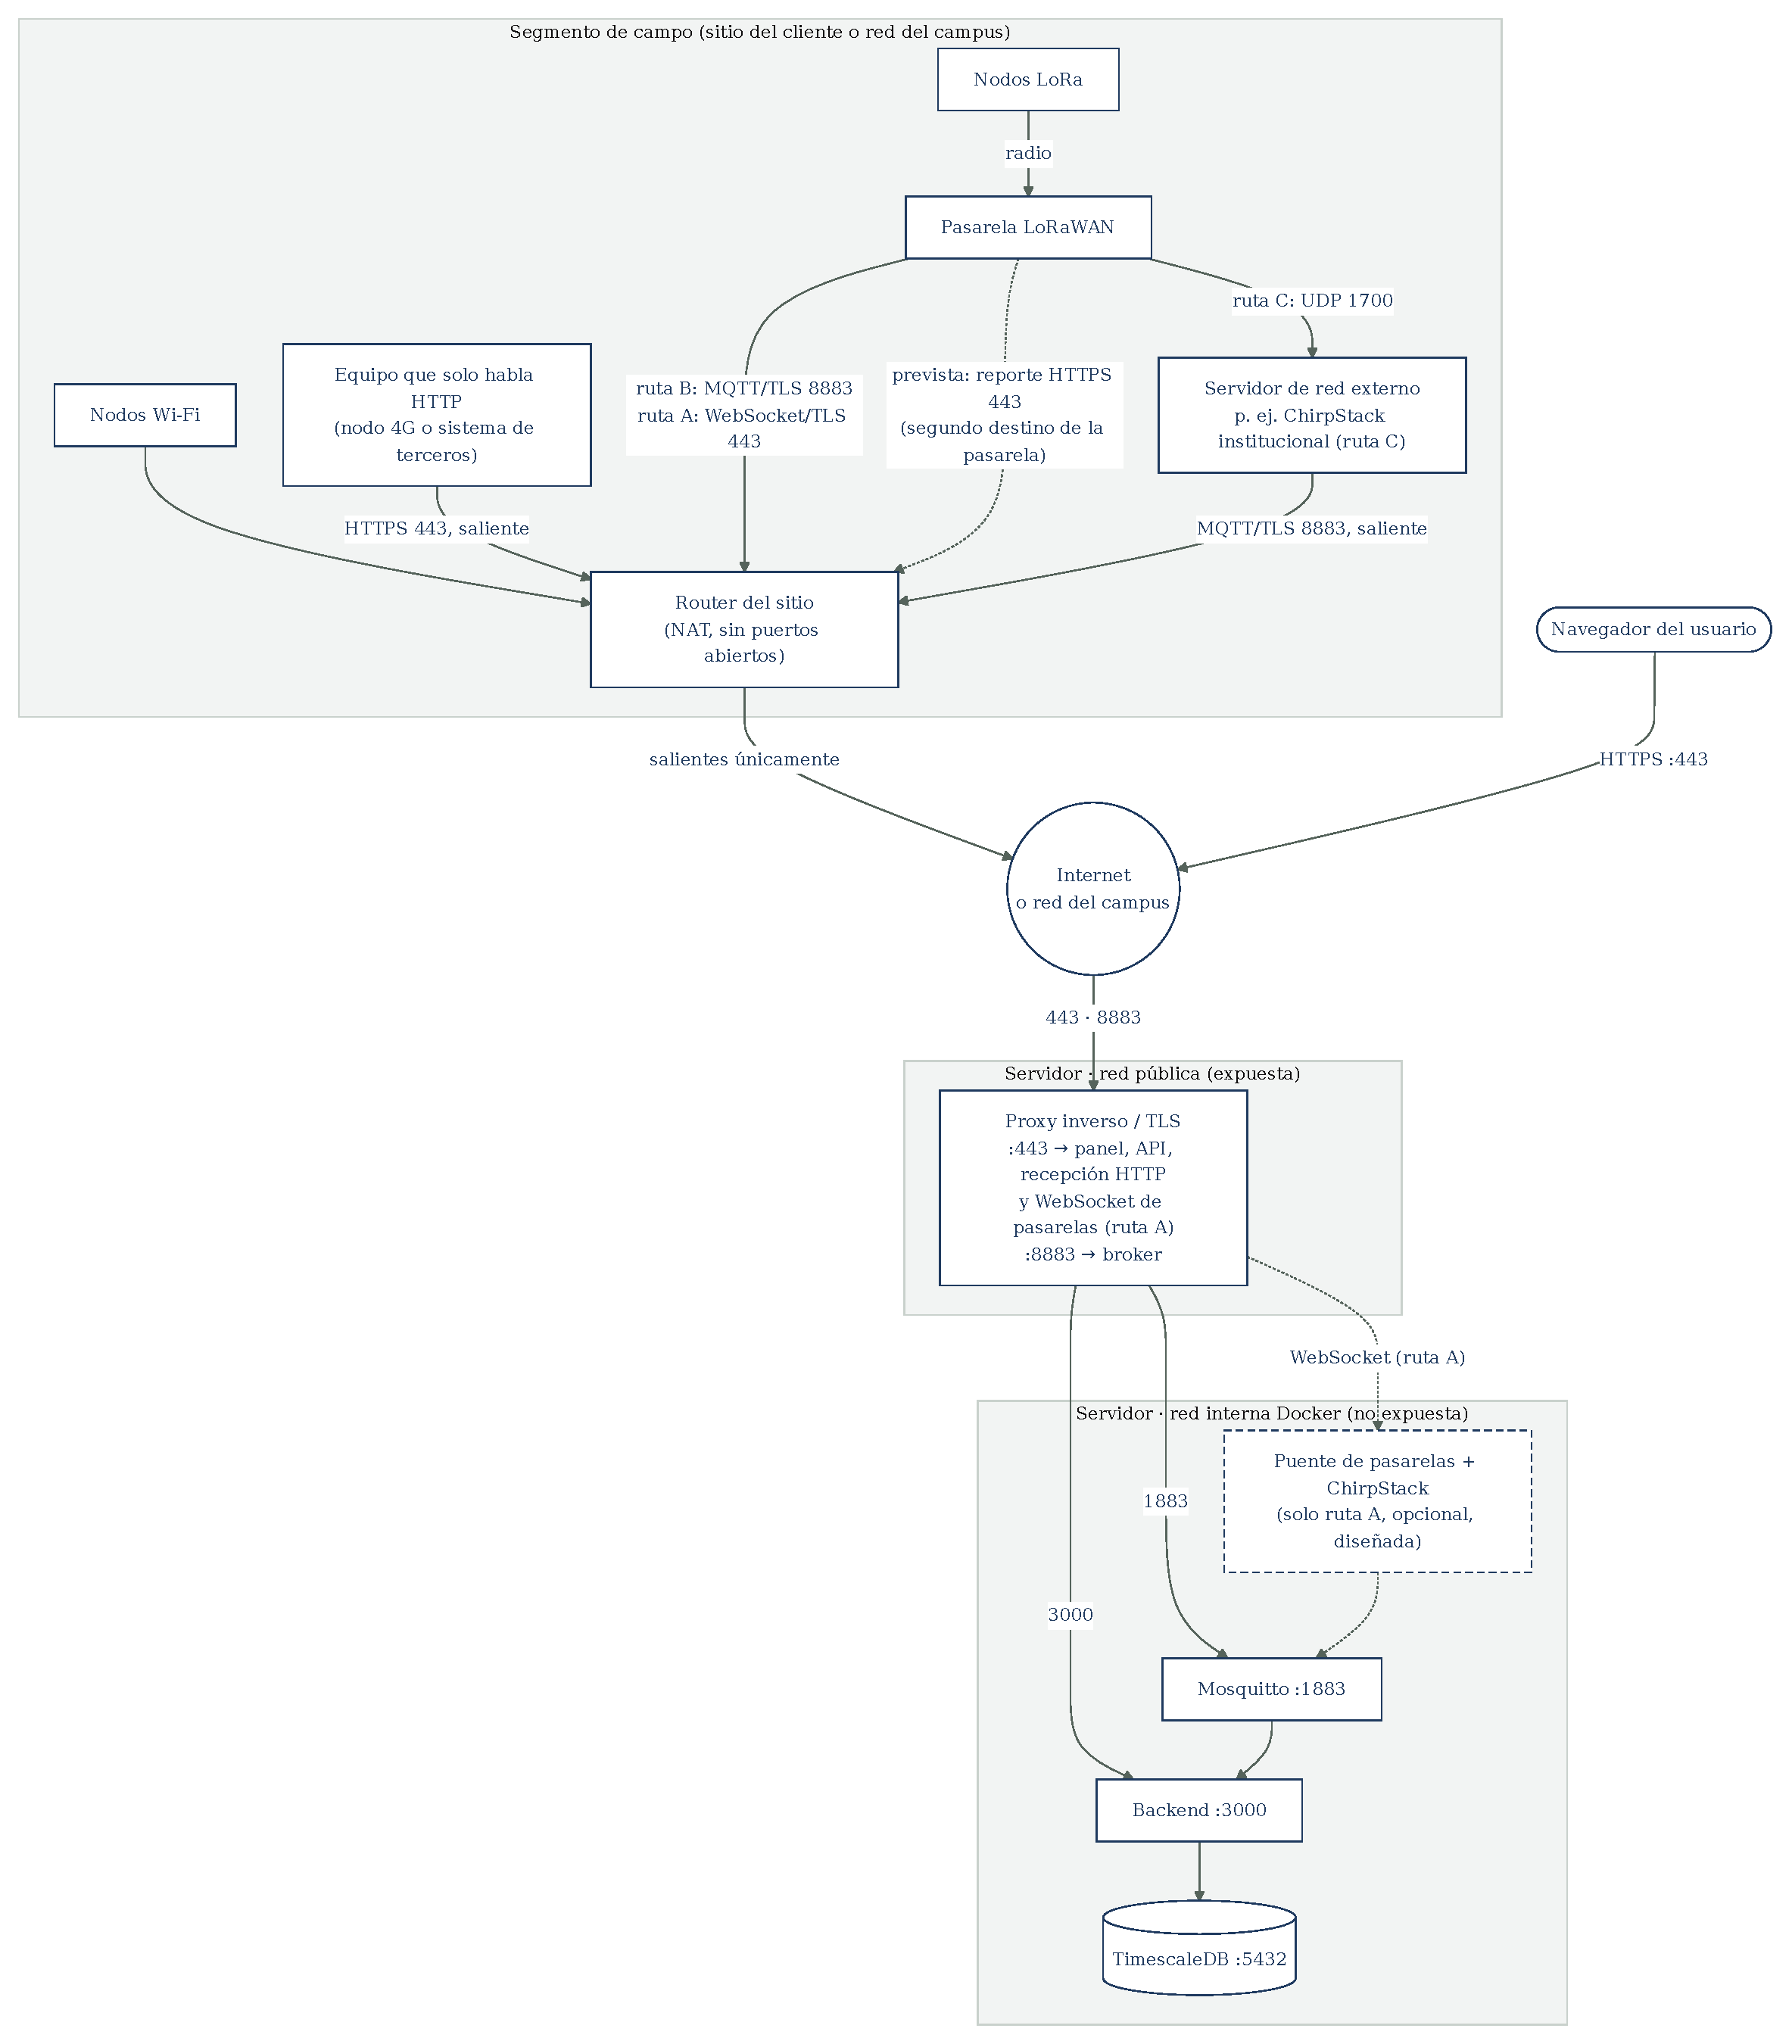
\includegraphics[width=\linewidth,height=0.85\textheight,keepaspectratio]{figuras/render/red.pdf}
\caption{Topología de red y segmentación. Los dispositivos del sitio solo abren conexiones \emph{salientes}: el router del cliente no necesita puertos abiertos ni configuración (RNF-10). Las tres vías de entrada (MQTT sobre TLS, HTTPS y, diseñada y punteada, WebSocket sobre TLS para la pasarela con \emph{Basics Station}) y el reporte HTTPS previsto de la pasarela cruzan el mismo router. En el servidor, únicamente el proxy con TLS es alcanzable desde Internet, siempre en 443 y 8883; broker, backend, base de datos y, si existe, ChirpStack (opcional, ruta A) viven en la red interna de los contenedores.}
\label{fig:red}
\end{figure}


\begin{sidewaysfigure}
\centering
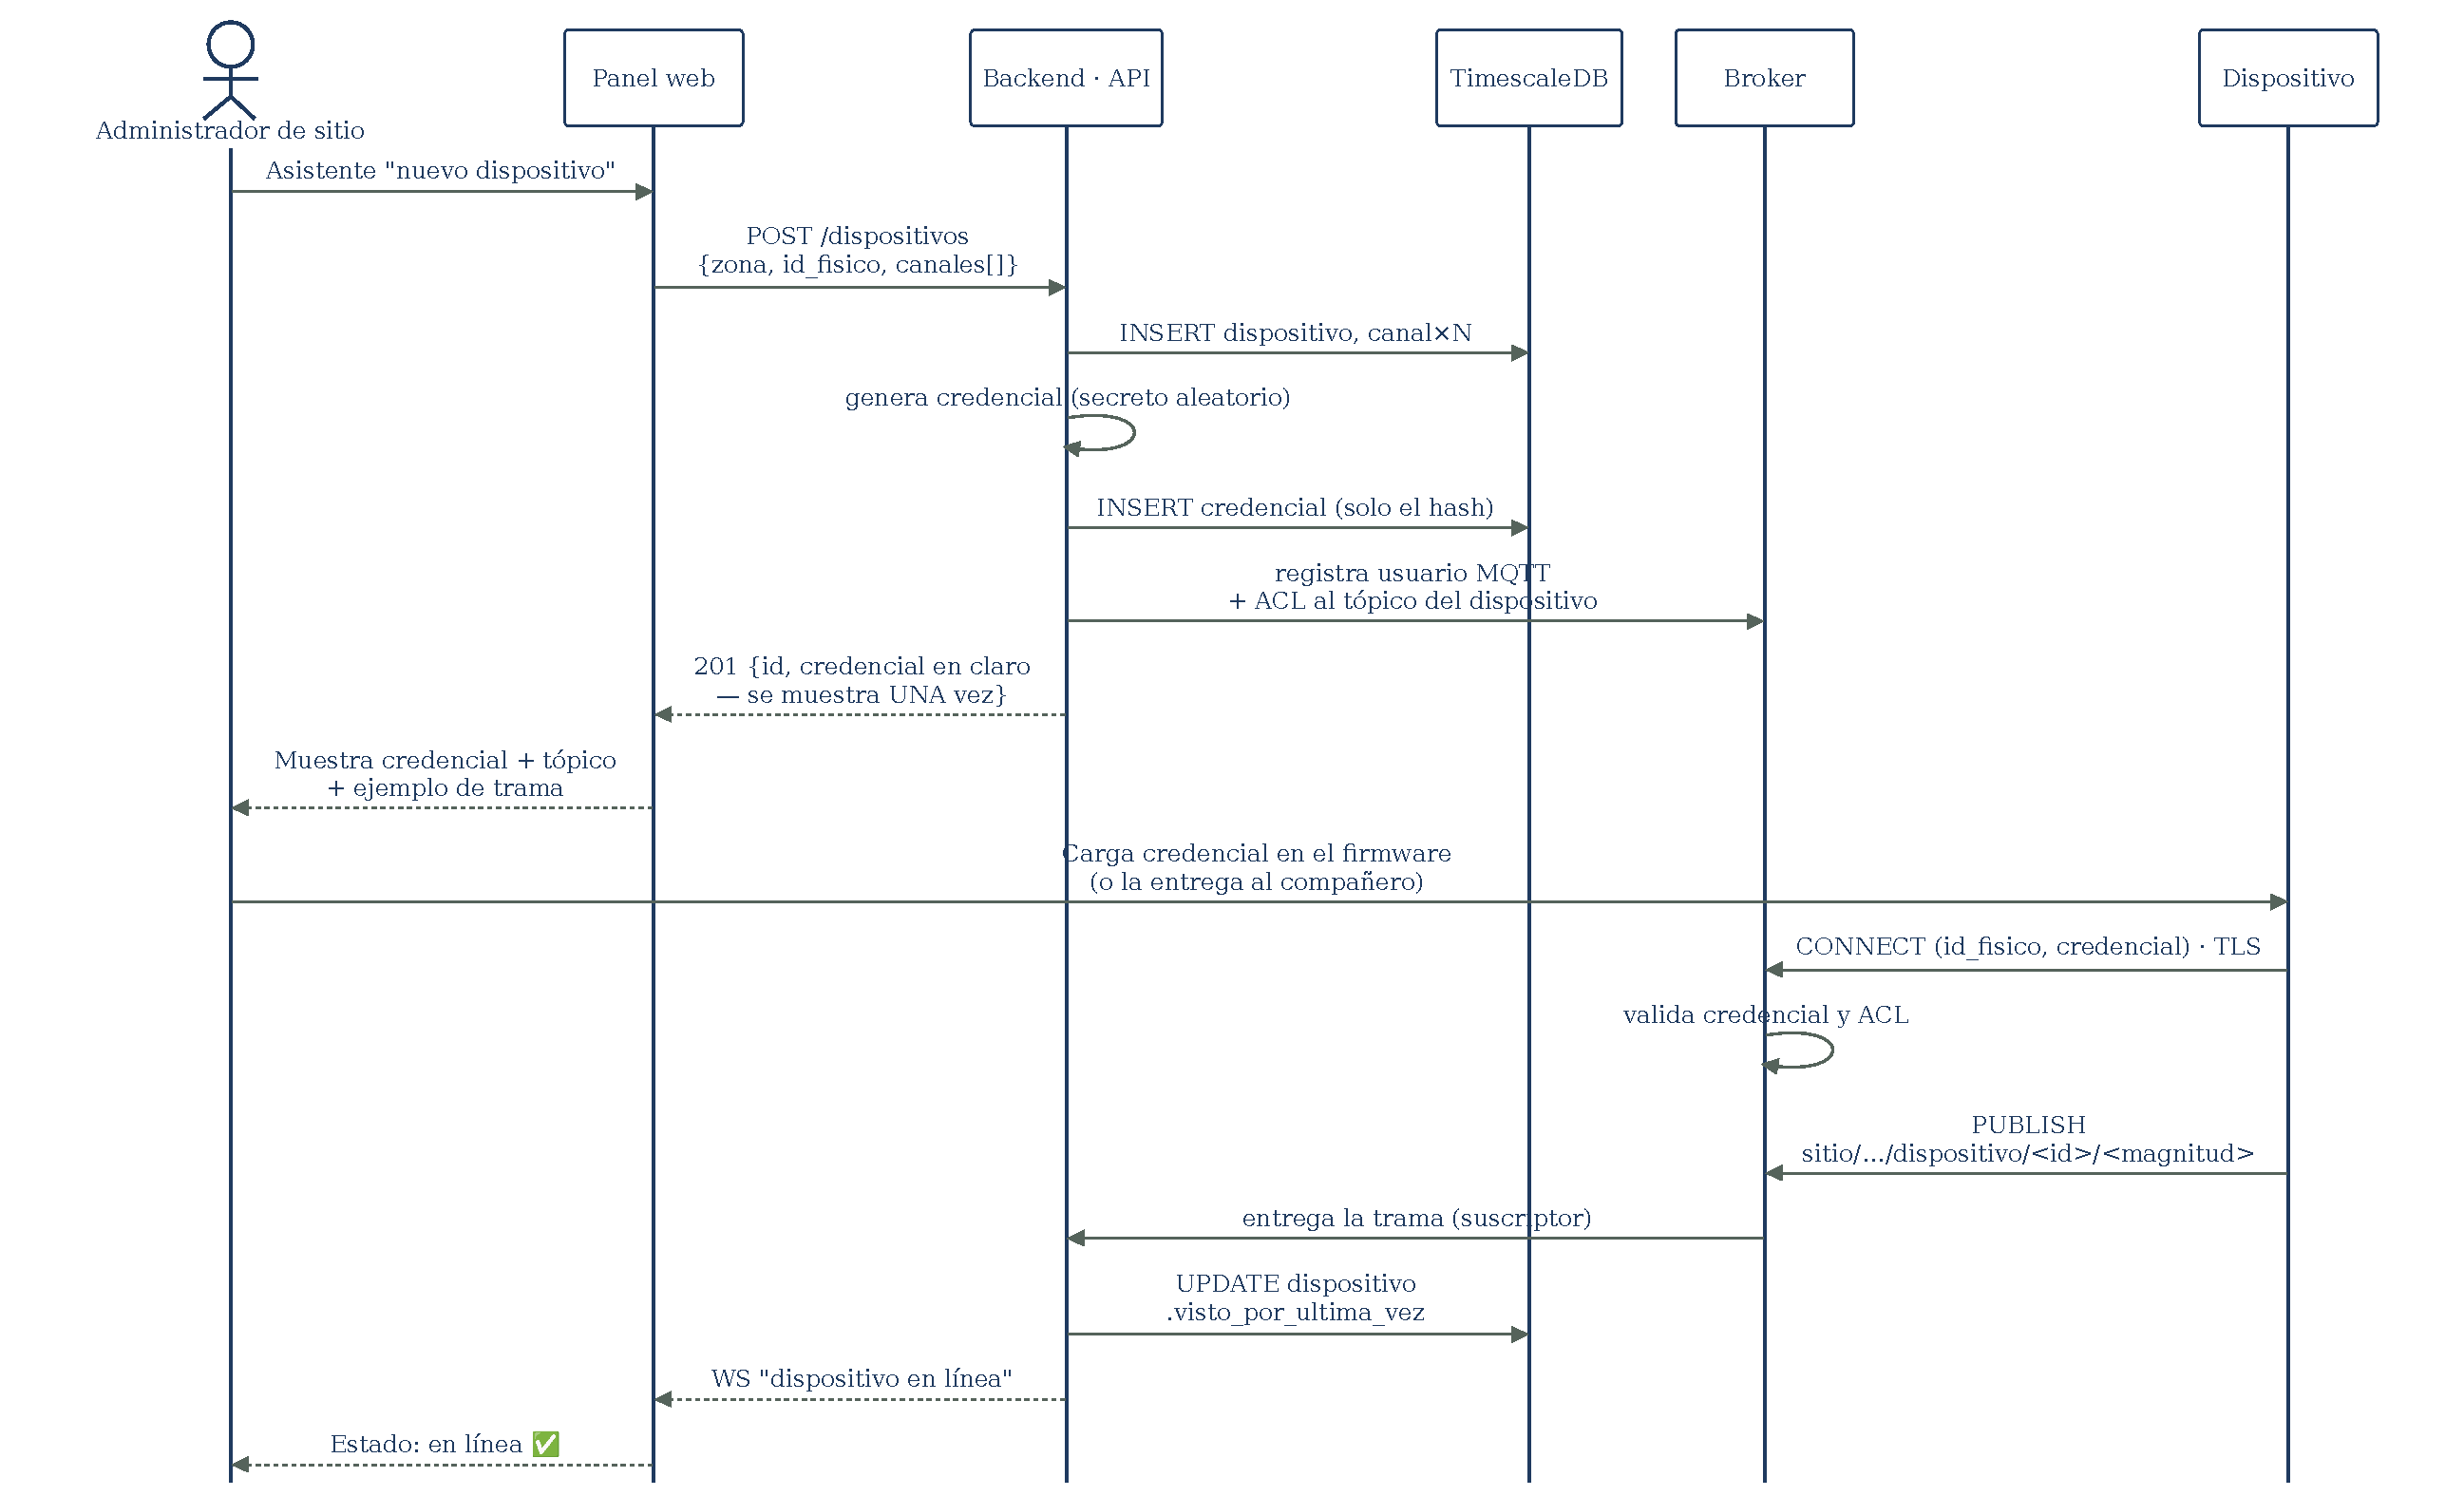
\includegraphics[width=0.96\textheight,height=0.9\textwidth,keepaspectratio]{figuras/render/sec-alta.pdf}
\caption{Aprovisionamiento de un dispositivo (diagrama de secuencia UML). Según la vía declarada (MQTT, HTTP o LoRaWAN, que autentica su pasarela), la credencial se genera en el servidor, se muestra una sola vez y en la base queda solo su hash; la ACL del broker limita al dispositivo a su propio tópico. Es el flujo que ataca la causa C4: una persona sin perfil técnico da de alta un sensor desde el panel. La ruta \texttt{POST /dispositivos} está implementada (Etapa 3); el alta desde el panel es de la Etapa 4.}
\label{fig:sec-alta}
\end{sidewaysfigure}


\begin{figure}[!htb]
\centering
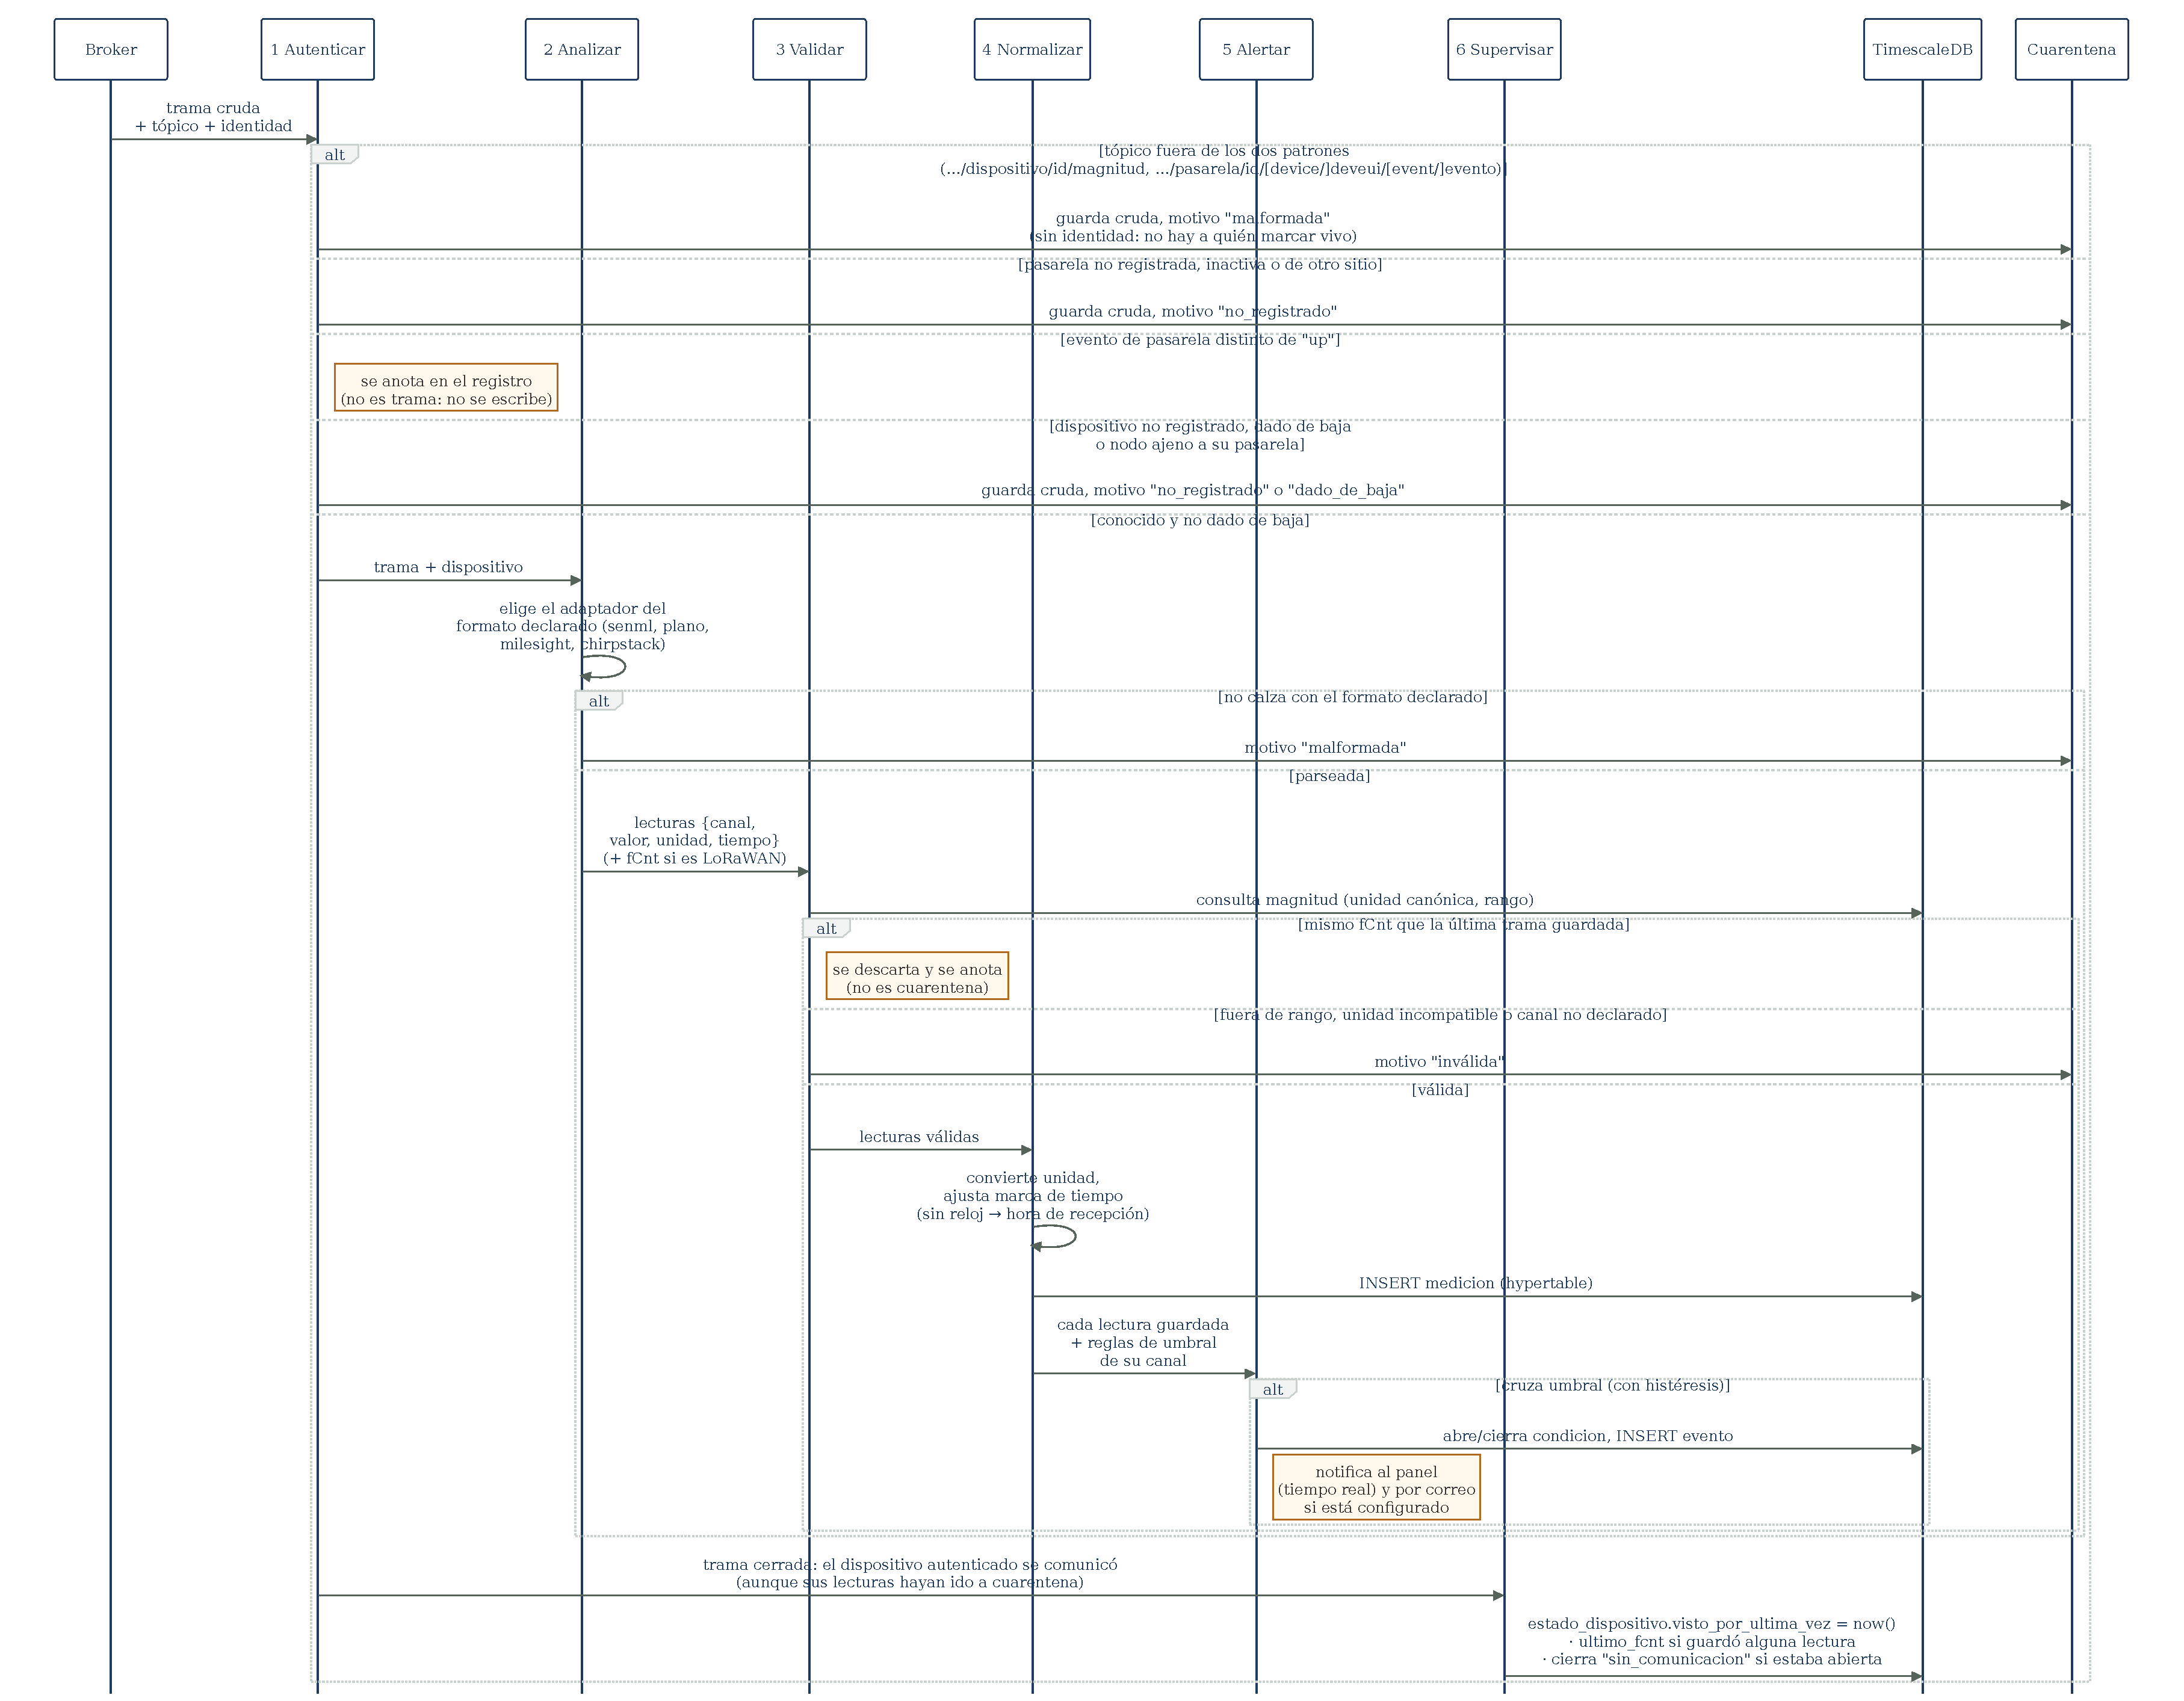
\includegraphics[width=\linewidth,keepaspectratio]{figuras/render/sec-pipeline.pdf}
\caption{Recepción de una trama: el pipeline de seis filtros como diagrama de secuencia UML. Cada filtro tiene una salida que continúa y una de rechazo hacia la cuarentena; ninguna trama llega a las series de tiempo sin superar los seis.}
\label{fig:sec-pipeline}
\end{figure}


\begin{figure}[!htb]
\centering
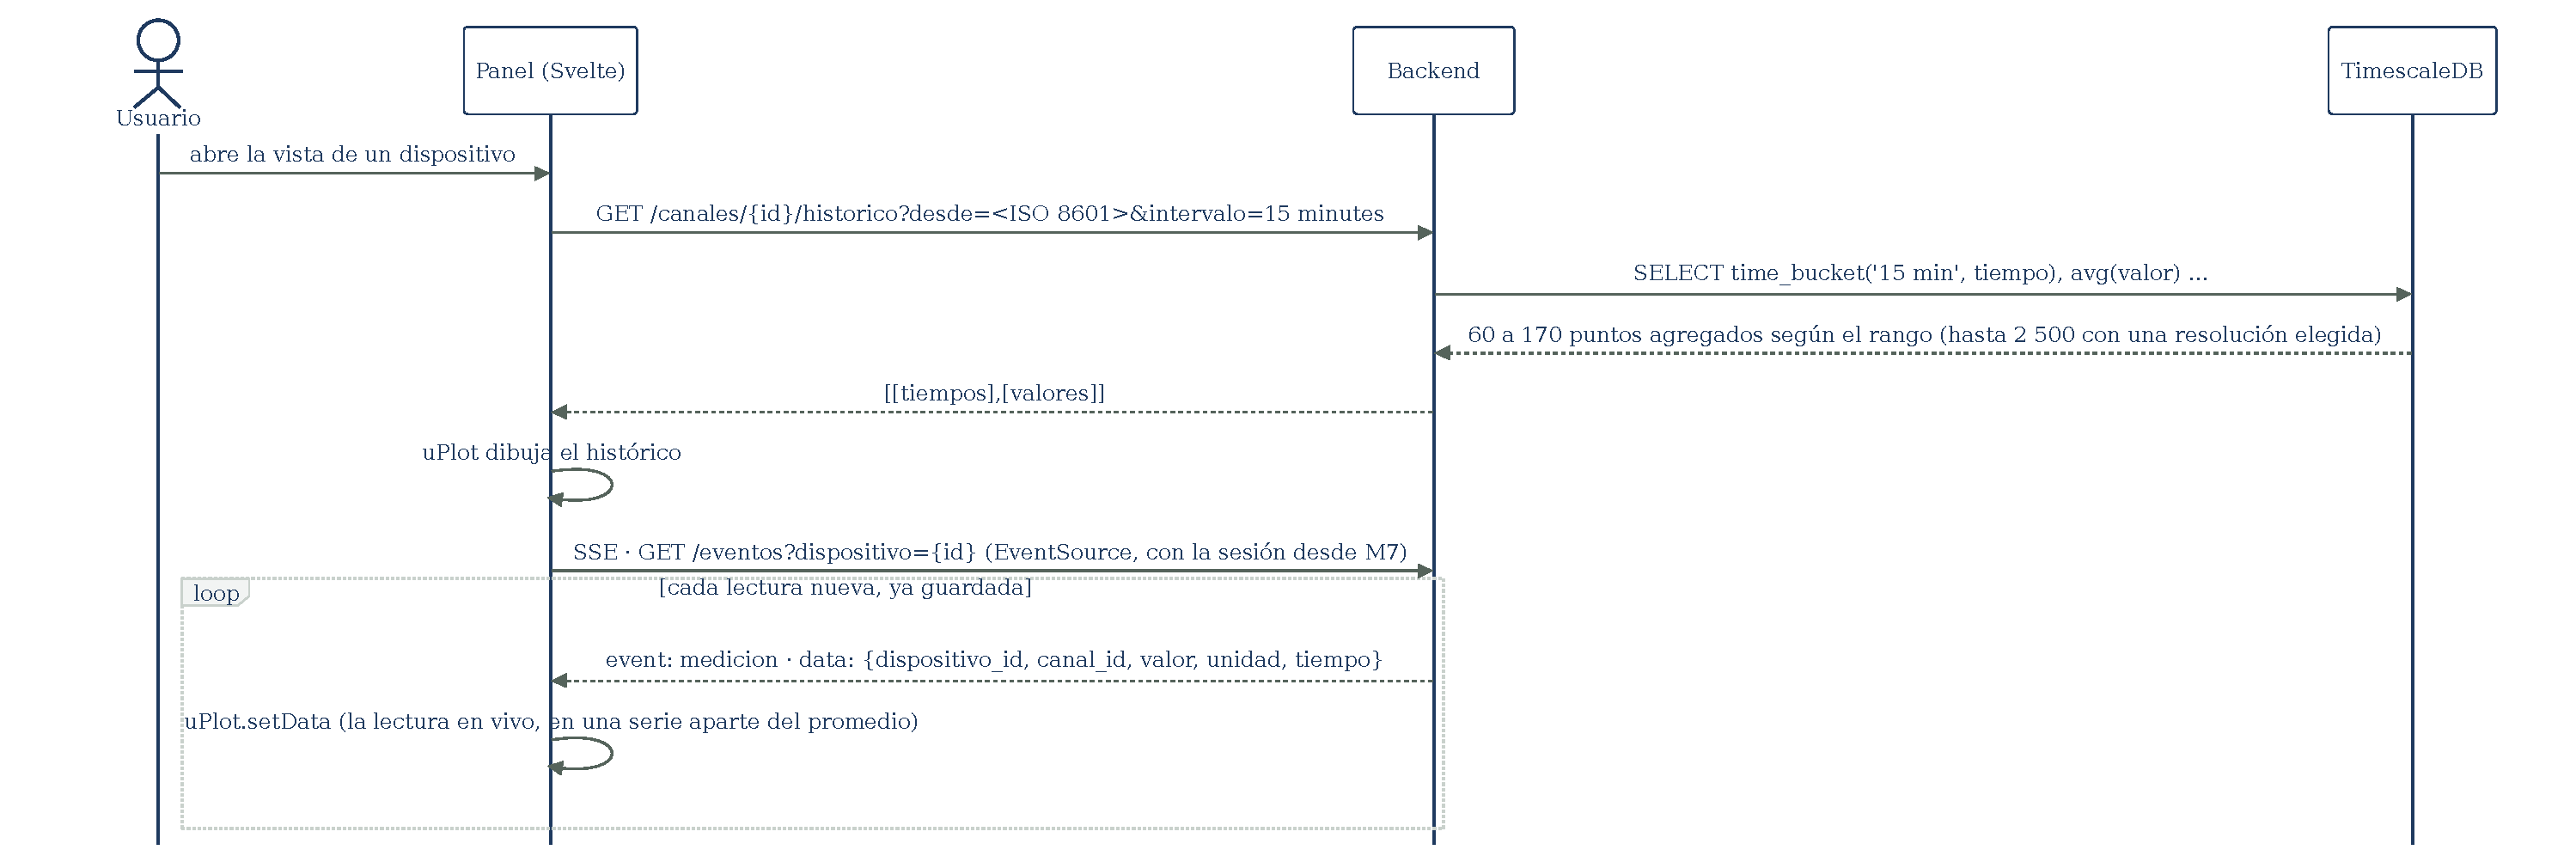
\includegraphics[width=0.78\linewidth,keepaspectratio]{figuras/render/sec-tiemporeal.pdf}
\caption{Panel en tiempo real (patrón B). El histórico llega agregado por la base de datos en la zona horaria del sitio —cientos de puntos, no millones— y las lecturas nuevas se empujan por WebSocket desde el backend.}
\label{fig:sec-tiemporeal}
\end{figure}


\begin{figure}[htbp]
\centering
\resizebox{0.98\linewidth}{!}{%
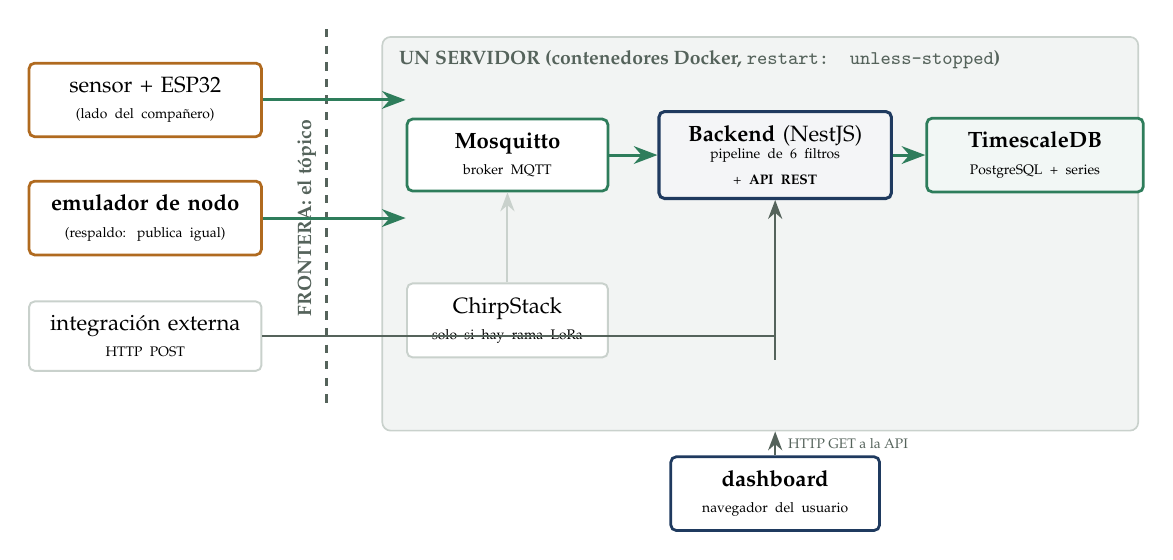
\begin{tikzpicture}[font=\scriptsize]

% lado emisores
\node[caja, text width=2.6cm, align=center, draw=ambar, line width=1pt] (n1) at (0,1.7)
  {sensor + ESP32\\ \tiny (lado del compañero)};
\node[caja, text width=2.6cm, align=center, draw=ambar, line width=1pt] (n2) at (0,0.2)
  {\textbf{emulador de nodo}\\ \tiny (respaldo: publica igual)};
\node[caja, text width=2.6cm, align=center, draw=grislinea] (n3) at (0,-1.3)
  {integración externa\\ \tiny HTTP POST};

% frontera
\draw[line width=1pt, color=gristexto, dashed] (2.3,2.6) -- (2.3,-2.2);
\node[etiqueta, font=\scriptsize\bfseries\color{gristexto}, rotate=90] at (2.05,0.2) {FRONTERA: el tópico};

% servidor
\node[grupo, minimum width=9.6cm, minimum height=5.0cm, anchor=west] (srv) at (3.0,0) {};
\node[font=\scriptsize\bfseries\color{gristexto}, anchor=north west] at (3.1,2.45)
  {UN SERVIDOR (contenedores Docker, \texttt{restart: unless-stopped})};

\node[caja, text width=2.2cm, align=center, draw=verdeacento, line width=1pt] (mq) at (4.6,1.0)
  {\textbf{Mosquitto}\\ \tiny broker MQTT};
\node[caja, text width=2.2cm, align=center, draw=grislinea] (cs) at (4.6,-1.1)
  {ChirpStack\\ \tiny solo si hay rama LoRa};
\node[caja, text width=2.6cm, align=center, draw=azuloscuro, line width=1.1pt, fill=azuloscuro!5] (be) at (8.0,1.0)
  {\textbf{Backend} (NestJS)\\ \tiny pipeline de 6 filtros\\ \tiny + \textbf{API REST}};
\node[caja, text width=2.4cm, align=center, draw=verdeacento, line width=1pt, fill=verdeacento!6] (db) at (11.3,1.0)
  {\textbf{TimescaleDB}\\ \tiny PostgreSQL + series};

\draw[flechagruesa] (n1.east) -- (mq.west|-n1.east);
\draw[flechagruesa] (n2.east) -- (mq.west|-n2.east);
\draw[flecha] (n3.east) -| (8.0,-1.6) -- (be.south);
\draw[flechagruesa] (mq.east) -- (be.west);
\draw[flecha, color=grislinea] (cs.north) -- (mq.south);
\draw[flechagruesa] (be.east) -- (db.west);

% dashboard afuera
\node[caja, text width=2.3cm, align=center, draw=azuloscuro, line width=1pt] (dash) at (8.0,-3.3)
  {\textbf{dashboard}\\ \tiny navegador del usuario};
\draw[flecha] (dash.north) -- node[nota, right=1pt, font=\tiny] {HTTP GET a la API} (be.south|-srv.south);

\end{tikzpicture}}
\caption{Despliegue: todos los componentes corren como contenedores en un único servidor. La
frontera con el trabajo del compañero es el tópico MQTT; el emulador de nodo publica en el mismo
tópico, de modo que la validación no depende del hardware.}
\label{fig:despliegue}
\end{figure}


\begin{figure}[!htb]
\centering
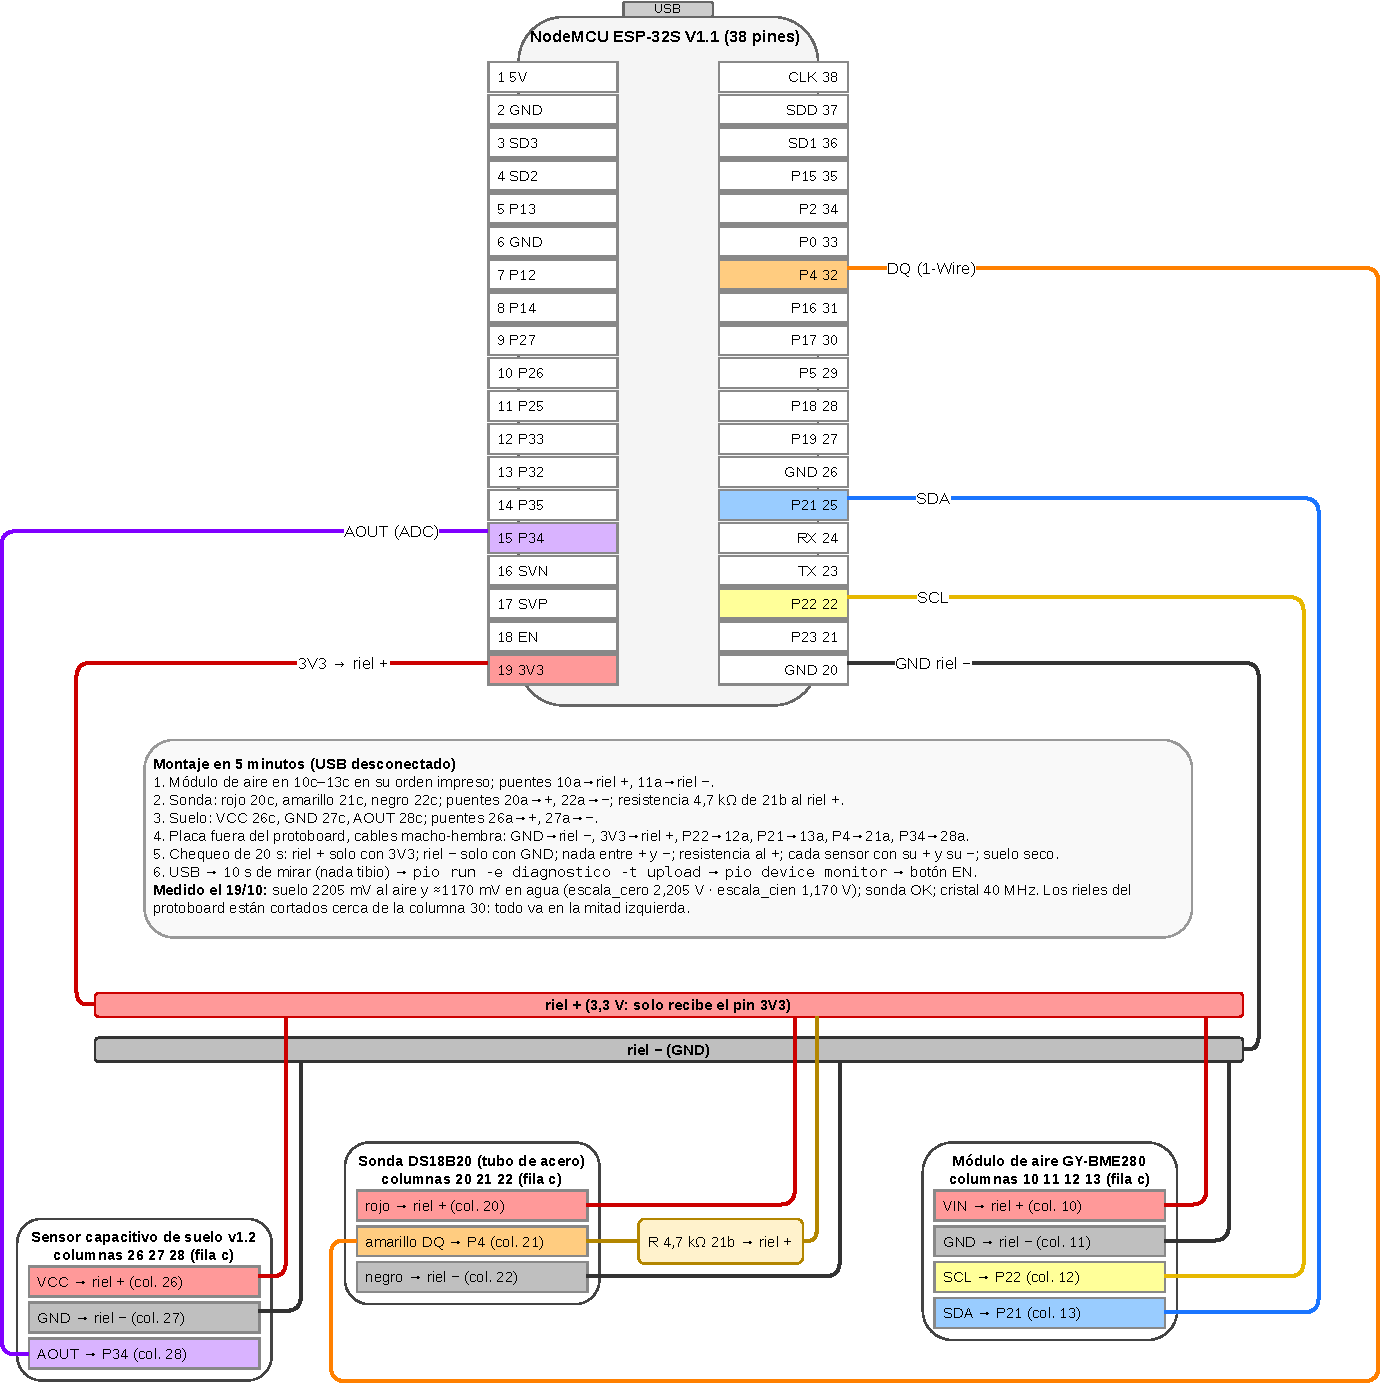
\includegraphics[width=\linewidth,height=0.78\textheight,keepaspectratio]{presentacion/figuras/cableado-esp32.pdf}
\caption[Cableado del nodo propio (fase 1)]{Cableado del nodo propio (fase 1, verificado el 19 de octubre de 2026): placa NodeMCU ESP-32S de 38 pines con el módulo de aire BME280 (I2C: SDA en P21, SCL en P22), la sonda de temperatura DS18B20 en tubo de acero (1-Wire en P4, con resistencia de 4,7~k$\Omega$ al riel de 3,3~V) y el sensor capacitivo de humedad de suelo (analógico en P34), sobre una protoboard cuyos rieles reciben solo 3,3~V y tierra desde la placa. Se cablea sin corriente y se revisa antes de conectar el USB; los pines están verificados contra el firmware. Dibujo del autor (\texttt{plataforma/firmware/cableado-fase-1.drawio}); montaje, calibración y compra en \texttt{docs/17}.}
\label{fig:cableado}
\end{figure}


\chapter[Camino descartado: Contact ID]{Camino evaluado y descartado: el protocolo Contact ID}
\label{anx:contactid}
\small

Durante la fase inicial de esta etapa (17 de agosto al 1 de septiembre) el trabajo evaluó como eje el
protocolo \textbf{Contact ID (SIA DC-05)} de la industria de alarmas, sobre transporte DC-09. Se
verificó empíricamente su gramática y su suma de comprobación con una implementación propia, se
evaluaron ocho alternativas mediante una matriz ponderada y se diseñó un perfil de aplicación. Ese
material completo permanece en el repositorio del proyecto (\texttt{docs/05-protocolo-contactid.md} y
\texttt{plataforma/herramientas/contactid.py}).

\textbf{Razón del descarte (reunión con el profesor guía, 2 de septiembre de 2026):} Contact ID está
orientado a \textbf{eventos discretos} —alarmas que ocurren o no— mientras que el problema de este
trabajo es \textbf{telemetría continua}: lecturas periódicas cada 5 a 30 minutos cuyo valor está en
la serie, no en el evento. El mensaje de 16 dígitos no transporta valores medidos de forma nativa, y
las extensiones necesarias para hacerlo desplazaban al protocolo fuera de su dominio de diseño.

\textbf{Lo que el análisis aportó y se conserva:} la restricción de que el silencio de un sensor
debe detectarse activamente (los códigos de supervisión de la industria de alarmas inspiran los
requerimientos RF-24 a RF-30, hoy resueltos con el \emph{keep-alive} y el testamento de MQTT); la
disciplina de evaluar alternativas con criterios ponderados y de verificar afirmaciones con código; y
la separación lógica entre eventos y telemetría, que sobrevive dentro del modelo interno.

El registro de la decisión, con las tareas derivadas, está en
\texttt{bitacora/2026-09-02-reunion-pivote.md}.

\chapter[Despliegue de prueba en la institución]{Despliegue de prueba en la institución: procedimiento, hallazgos y proyección}
\label{anx:despliegue}

Complementa la sección~\ref{sec:despliegue-prueba}: qué se pidió, qué se obtuvo, qué se midió, qué falló y qué queda, sin nombres,
direcciones ni credenciales, que viven fuera del repositorio (\texttt{docs/11 §7}). El procedimiento con el porqué de cada decisión está en
\texttt{docs/14 §7}; el registro de los dos días, en la bitácora del 3 y 4 de noviembre.

\section{Qué se pidió y qué se obtuvo}

Lo que el diseño necesitaba de la institución era concreto: un equipo con Linux y Docker en su red, o un espacio en un clúster, con un
puerto de entrada para dispositivos (8883) y, a futuro, un nombre público para el certificado. La universidad ofreció un equipo de su red el 1 de
noviembre; el 3 llegaron dos cosas distintas de lo planeado: acceso a un \textbf{namespace de Kubernetes} de uso estudiantil y un
\textbf{equipo compartido} en la red del campus, que ya tenía responsable, un servicio de otro proyecto corriendo y acceso remoto solo con llave.
La regla fue medir primero y diseñar después: en los dos entornos se hicieron pruebas baratas y borrables antes de instalar nada.

\section{El namespace: lo que cabe, lo que falta y lo que llega}

Diecisiete pruebas, de solo lectura o con recursos etiquetados y borrados al terminar, respondieron cuatro preguntas (cuadro~\ref{tab:namespace}).

\begin{table}[H]
\centering\footnotesize
\begin{tablaseg}
\begin{tabular}{@{}L{2.6cm}L{6.4cm}L{4cm}@{}}
\toprule
\textbf{Pregunta} & \textbf{Resultado} & \textbf{Qué implica} \\
\midrule
¿Cabe la pila? & La cuota (2 CPU y 2~GB) y los permisos del namespace bastan para la pila, que mide 193~MiB en reposo y 324 en pico; los manifiestos de prueba, escritos para el perfil de seguridad restringido, pasan la admisión; los pods ejecutan en nodos reales y descargan imágenes públicas; la administración remota funciona sin exponer nada. & Sirve como entorno de desarrollo y de integración. \\
¿Se llega desde afuera? & No hay clase de \emph{Ingress} ni balanceador asignado, y las direcciones de nodo viven en una red que ni la red del campus enruta (medido desde la red de la pasarela: tiempo agotado). & Sin puerta de entrada ningún dispositivo publica. Pedida al administrador. \\
¿Se puede guardar? & No quedaba cupo de volúmenes persistentes disponible. & Sin volúmenes no hay base ni broker con estado. Pedido cupo. \\
¿Llega al campus? & Hay conectividad en el sentido clúster $\rightarrow$ campus, no en el inverso. & El diseño necesita el inverso: la pasarela publica al broker. \\
\bottomrule
\end{tabular}
\end{tablaseg}
\caption[El namespace medido antes de diseñar]{El namespace medido el 3 de noviembre de 2026, antes de diseñar.}
\label{tab:namespace}
\end{table}

Conclusión: el namespace ejecuta la plataforma pero no la deja operar. Las dos carencias dependen de la administración del clúster y se pidieron con la evidencia de cada prueba. Se descartó resolverlo con rodeos, como un puente de salida hacia un broker ajeno: el sistema funciona como está diseñado.

\section{El equipo compartido: reglas y procedimiento}

La lista de aceptación de \texttt{docs/14 §7.1} (soporte de seguridad vigente, administración delegada, nada sin explicar, disco sano,
actualizable) se aplicó con una diferencia: los usuarios y servicios ajenos los explicó su responsable, presente, y el equipo se acepta como
compartido. Reglas acordadas: un usuario propio con lo mínimo; acceso remoto solo con llave y solo por una red privada cifrada entre el portátil
del autor y el servidor; nada del anfitrión se toca (cortafuegos, demonio de Docker, parches y reinicios son del responsable); ningún comando
sobre contenedores ajenos; cada cambio avisado el mismo día, con el inventario de lo instalado y cómo deshacerlo.

El procedimiento, en orden: clon anónimo del repositorio público (actualiza, no empuja); secretos generados en el propio servidor, nunca
copiados de desarrollo; certificado emitido por una autoridad propia de este entorno, creada fuera del servidor y con su clave cifrada; forma de
producción de Compose, que publica solo los puertos del proxy y los de personas únicamente en la dirección de la red privada; construcción,
inicialización del broker con sus roles, y alta del sitio, de la pasarela del campus y de los dos nodos del compañero. Respaldo diario de la base, con restauración probada, y del archivo de credenciales del broker; copia fuera del servidor.

\section{Problemas que aparecieron y qué enseñaron}

\begin{itemize}
\item \textbf{El backend no arrancaba sano} hasta fijar la clave del rol de aplicación de la base, y el proxy, que espera a un backend sano,
  tampoco: era la señal correcta, no un error. Quedó como paso explícito del procedimiento.
\item \textbf{Un secreto no viaja como argumento de un comando:} si el comando falla, el intérprete lo imprime. Va por variable de entorno
  o se escribe sin eco.
\item \textbf{Un bloque de instalación escrito para una distribución y ejecutado en otra} dejó archivos vacíos: se descarga a un temporal
  y se comprueba antes de instalar.
\item \textbf{El reloj del servidor va en UTC:} la hora de «último acceso» se convierte a la hora local antes de interpretarla.
\item \textbf{Las credenciales de prueba que se muestran en pantalla se invalidan en el acto}, y los dispositivos de prueba se dan de baja
  al terminar.
\item \textbf{Una conexión tiene dirección:} sin dirección de entrada nadie llega, y las puertas y el disco los concede la institución.
  Una tarde de pruebas baratas dijo exactamente qué pedir y a quién.
\end{itemize}

\section{Verificado en ejecución el 4 de noviembre}

\begin{table}[H]
\centering\footnotesize
\begin{tablaseg}
\begin{tabular}{@{}L{5.2cm}L{7.8cm}@{}}
\toprule
\textbf{Afirmación} & \textbf{Resultado} \\
\midrule
Publicar por MQTT con TLS y por HTTPS con token & Guardado y visible en el panel \\
Sin credencial, o con credencial incorrecta & Rechazado; el broker lo registra \\
Sin TLS al 8883 & Rechazado \\
Sin token, o con token falso & Rechazado (401) \\
Puertos alcanzables & Solo los del contrato: 8883 en todas las interfaces; 443, 80 y el acceso remoto únicamente por la red privada; broker, backend y base cerrados \\
TLS 1.1 & Rechazado; TLS 1.2 negocia \\
Baja de un dispositivo & Dispositivo y credencial quedan inactivos \\
Reinicio de los contenedores & Los cuatro sanos en un minuto \\
Respaldo & Restaurado en una base de prueba con los mismos conteos; temporizador diario activo; copia fuera del servidor \\
\bottomrule
\end{tabular}
\end{tablaseg}
\caption[Verificación en el servidor de prueba]{Verificación de extremo a extremo en el servidor de prueba (4 de noviembre de 2026).}
\label{tab:servidor-verificacion}
\end{table}

\section{Lo que falta y cómo enlaza con la Etapa 4}

\begin{itemize}
\item \textbf{Entrada desde Internet:} pedida a la institución (reenvío del 8883 y, si es posible, un nombre DNS, que habilita el certificado
  público con Let's Encrypt). Hasta entonces publican solo la pasarela del campus y los equipos de la red privada.
\item \textbf{Sesión y roles} (bloque 1 de la Etapa~4): hoy el panel y la API se alcanzan solo por la red privada.
\item \textbf{Riesgo aceptado del equipo compartido:} en un equipo compartido, la administración del anfitrión tiene por diseño acceso a secretos, base y respaldos; por eso los secretos son de este entorno, se rotan al dejarlo y solo se cargan datos de prueba. El cifrado en reposo del respaldo está pendiente y, mientras tanto, el respaldo no contiene datos de producción.
\item \textbf{Operación pendiente:} latido a un vigilante externo, reinicio del equipo con su responsable, instalación en un paso, y las
  tramas reales de la pasarela cuando su responsable la apunte al servidor.
\item \textbf{Proyección:} la Etapa~4 mantiene este servidor como entorno de prueba (iteración 0: operando con respaldo y aviso); la validación de RNF-17 y de las 72~horas de RNF-18 (OE5) se hace en el servidor de recursos modestos que se confirme. El namespace queda como diseño B (\texttt{docs/14 §6}): varias réplicas del backend con suscripciones compartidas de MQTT~5 y el estado en un lugar común, para cuando la institución conceda entrada y volúmenes. El costo de alojamiento está cotizado (\texttt{docs/14 §3}); el consumo en pesos por sitio es de la Etapa~4.
\end{itemize}

\end{document}
